\thispagestyle{appendixheader}
\stepcounter{app}
\setcounter{app_fig}{1}
\setcounter{app_tab}{1}
\setcounter{equation}{0}
\renewcommand\theequation{附\arabic{app}-\arabic{equation}}
<<<<<<< HEAD
\renewcommand\chaptername{附录}
\renewcommand\chaptername{Appendix}
\renewcommand\thechapter{附录\zhnum{app}}
=======
% \renewcommand\theequation{\Alph{app}.\arabic{equation}}
\renewcommand\chaptername{附录}
\renewcommand\chaptername{Appendix} 
\renewcommand\thechapter{附录\zhnum{app}} 
>>>>>>> c4bb8a8e4d07c80bffd10fe9aeb672bafe56fbee

\setcounter{chapter}{0}
\setcounter{section}{0}

<<<<<<< HEAD
%========================================
% 附录一：自研物镜补充分析
%========================================
\chapter{自研物镜补充分析}\label{chap:app1}
=======

\chapter{变色龙激光器}\label{chap:app1}{
\stepcounter{app}
>>>>>>> c4bb8a8e4d07c80bffd10fe9aeb672bafe56fbee
\setcounter{app_fig}{1}
\setcounter{app_tab}{1}

\begin{table}[htbp]
<<<<<<< HEAD
    \centering
    \bicaption{自研空气物镜的 Zemax 简化处方参数}{Simplified Zemax prescription of the self-designed air objective}
    \label{tab:obj_appendix_prescription}
    \begin{tabular}{c c c c c l}
        \toprule
        面号 & 曲率半径 / mm & 厚度 / mm & 材料 & 净口径 / mm & 备注 \\
        \midrule
        2  & 10.2485  & 6.2622 & H-ZLAF2A  & 4.7975  & 折射面 \\
        3  & 6.1201   & 4.2994 & H-FK95N   & 6.7196  & 折射面 \\
        5  & 48.9115  & 2.6964 & H-ZK10L   & 9.3400  & 折射面 \\
        7  & 10.1474  & 4.0144 & D-FK95-25 & 10.7598 & 折射面 \\
        9  & 11.5002  & 6.0277 & H-FK95N   & 10.0682 & 折射面 \\
        10 & -6.5179  & 6.9845 & D-K9GT    & 8.7767  & 折射面 \\
        12 & -4.6773  & 2.5528 & H-K5      & 5.5076  & 光阑面 \\
        13 & 9.3071   & 6.7420 & D-FK61    & 8.4923  & 折射面 \\
        15 & 686.2102 & 6.6326 & H-FK95N   & 13.7028 & 平折射面 \\
        16 & -20.3797 & 0      & ---       & 14.9117 & 像前 \\
        \bottomrule
    \end{tabular}
\end{table}

表~\ref{tab:obj_appendix_prescription} 给出了自研空气物镜在 Zemax 中采用的简化处方参数。由于正文中主要讨论了该物镜面向大视场扫描应用时的总体设计思路与核心性能指标，附录中进一步列出处方参数与补充像差结果，用于说明该设计并非停留在概念层面，而是已经完成了基于具体玻璃材料、曲率半径与净口径约束的初步光学建模。


\begin{figure}[htbp]
    \centering
    \begin{subfigure}[b]{0.46\textwidth}
        \centering
        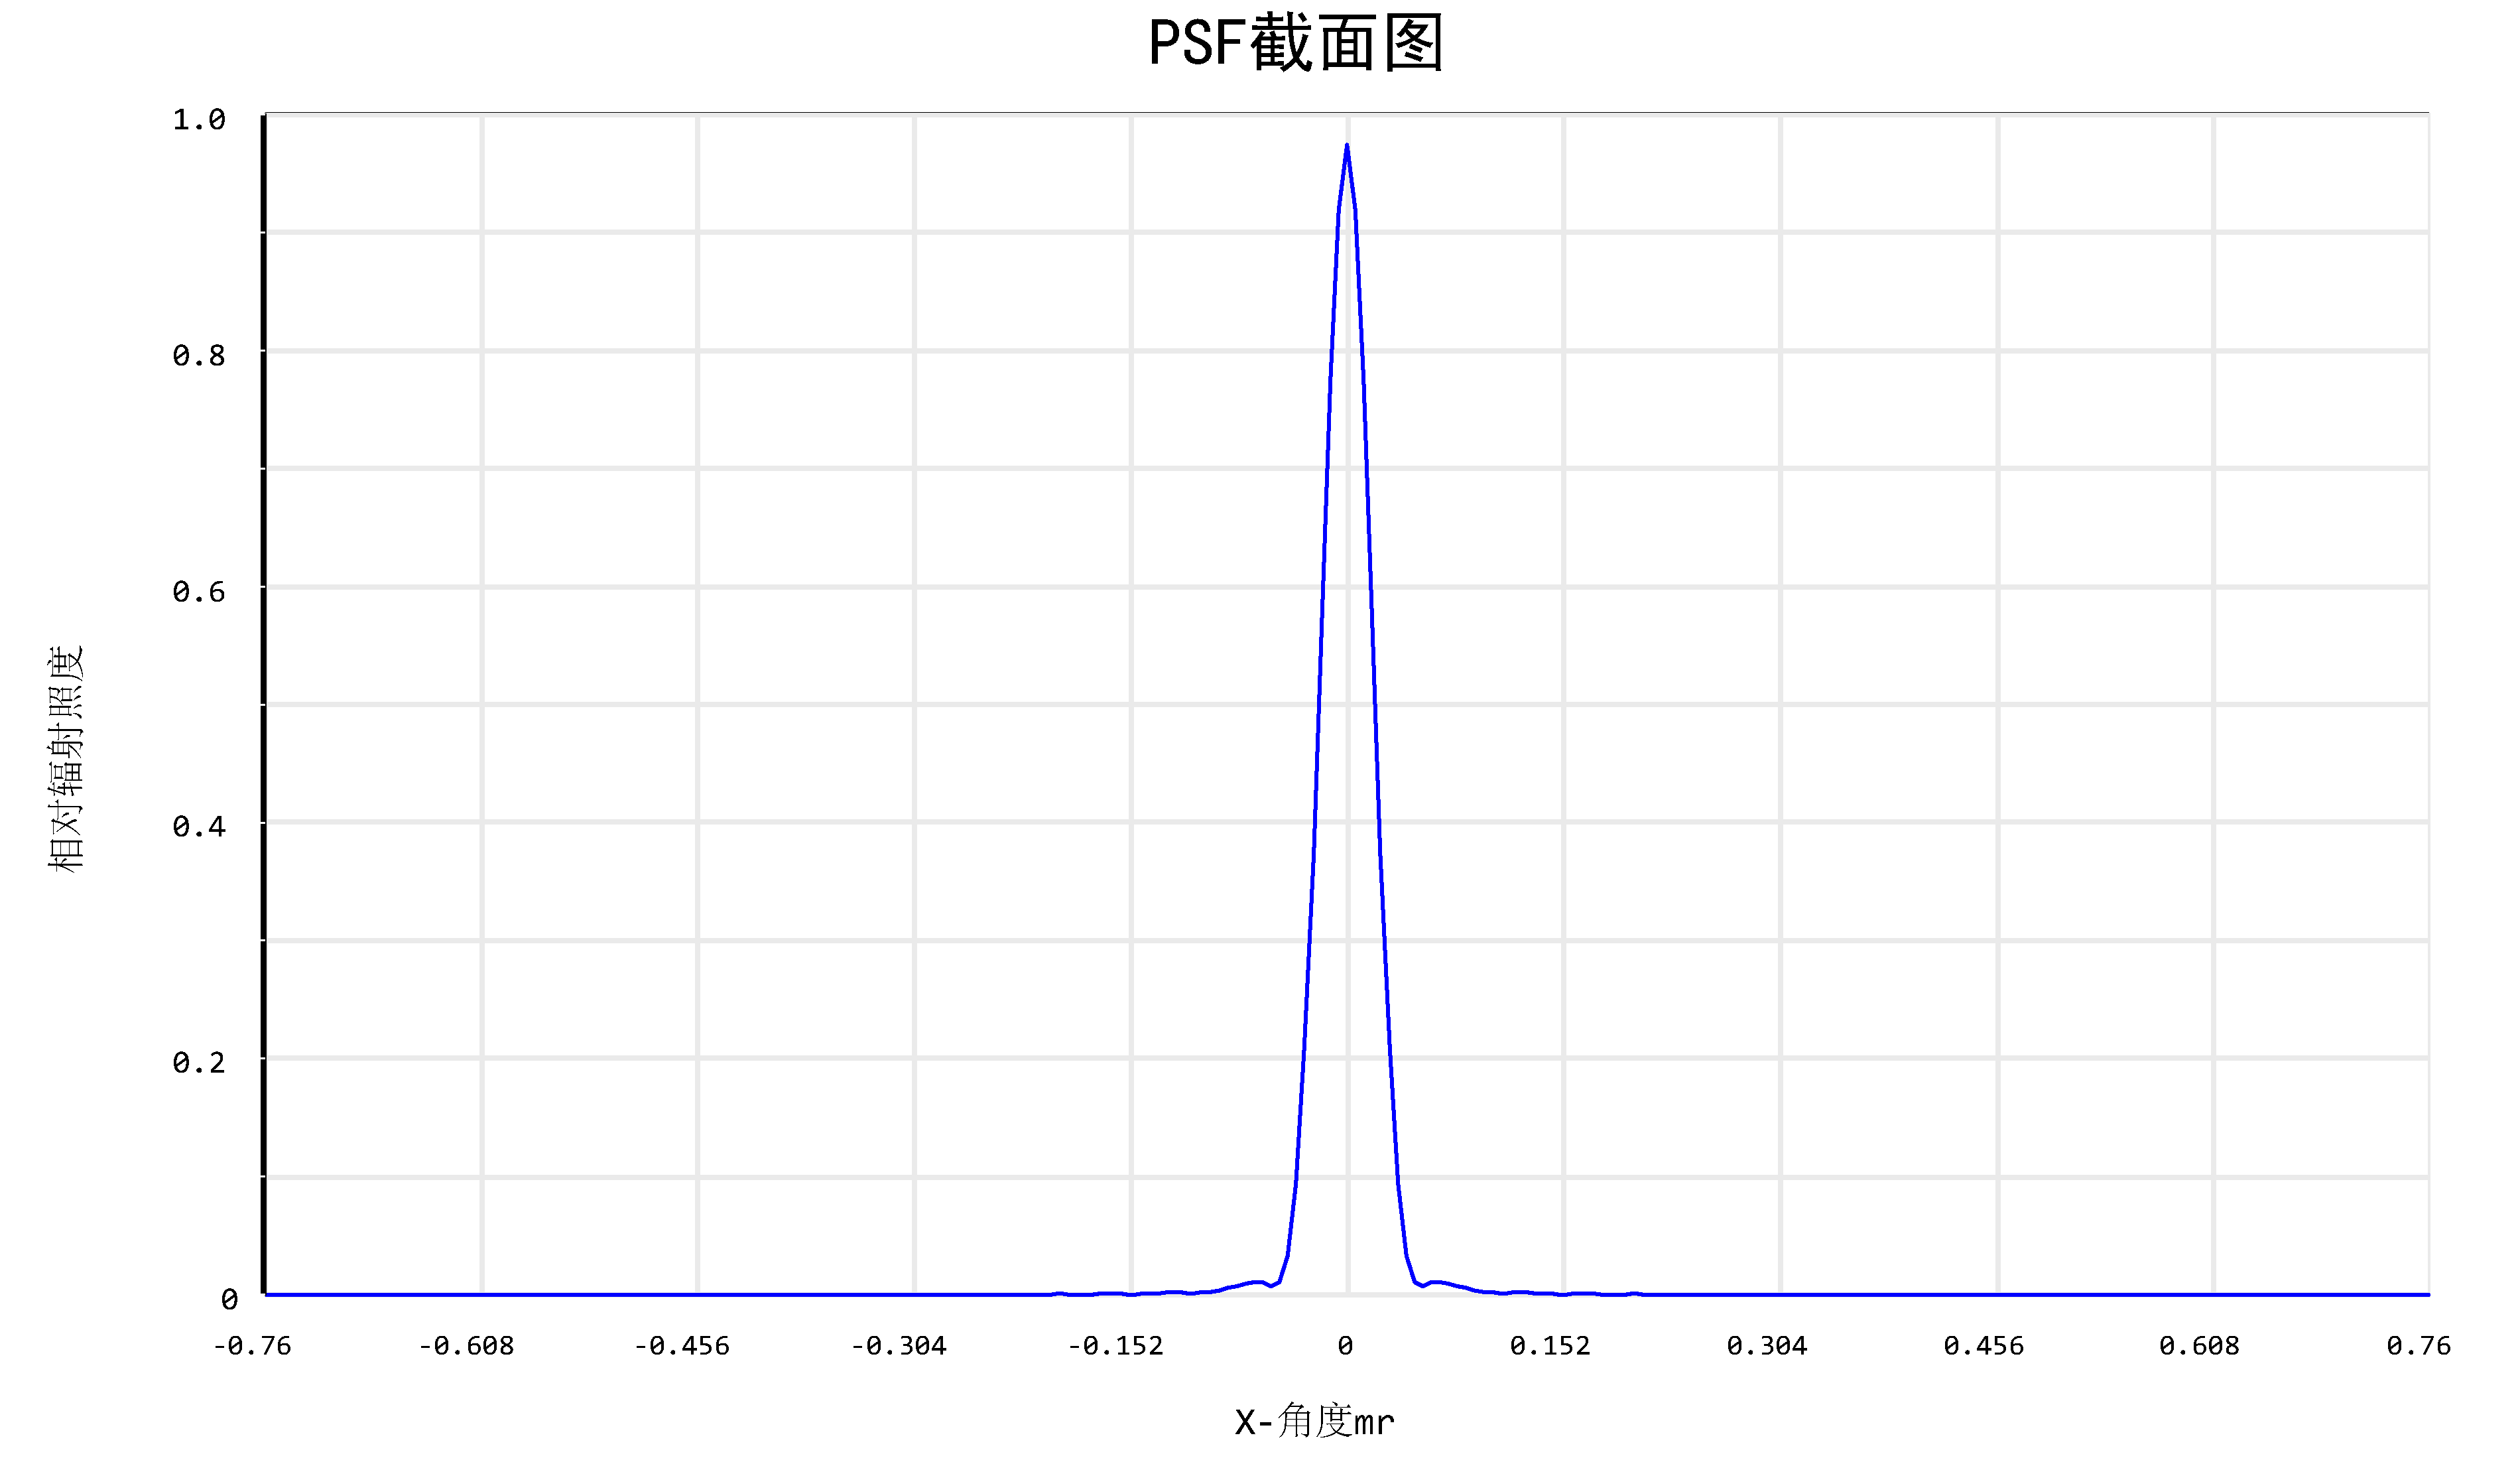
\includegraphics[width=\textwidth]{Fig/Fig-Obj-FFTPSF截面图.pdf}
        \caption{}
        \label{fig_obj_f}
    \end{subfigure}
    \hfil
    \begin{subfigure}[b]{0.49\textwidth}
        \centering
        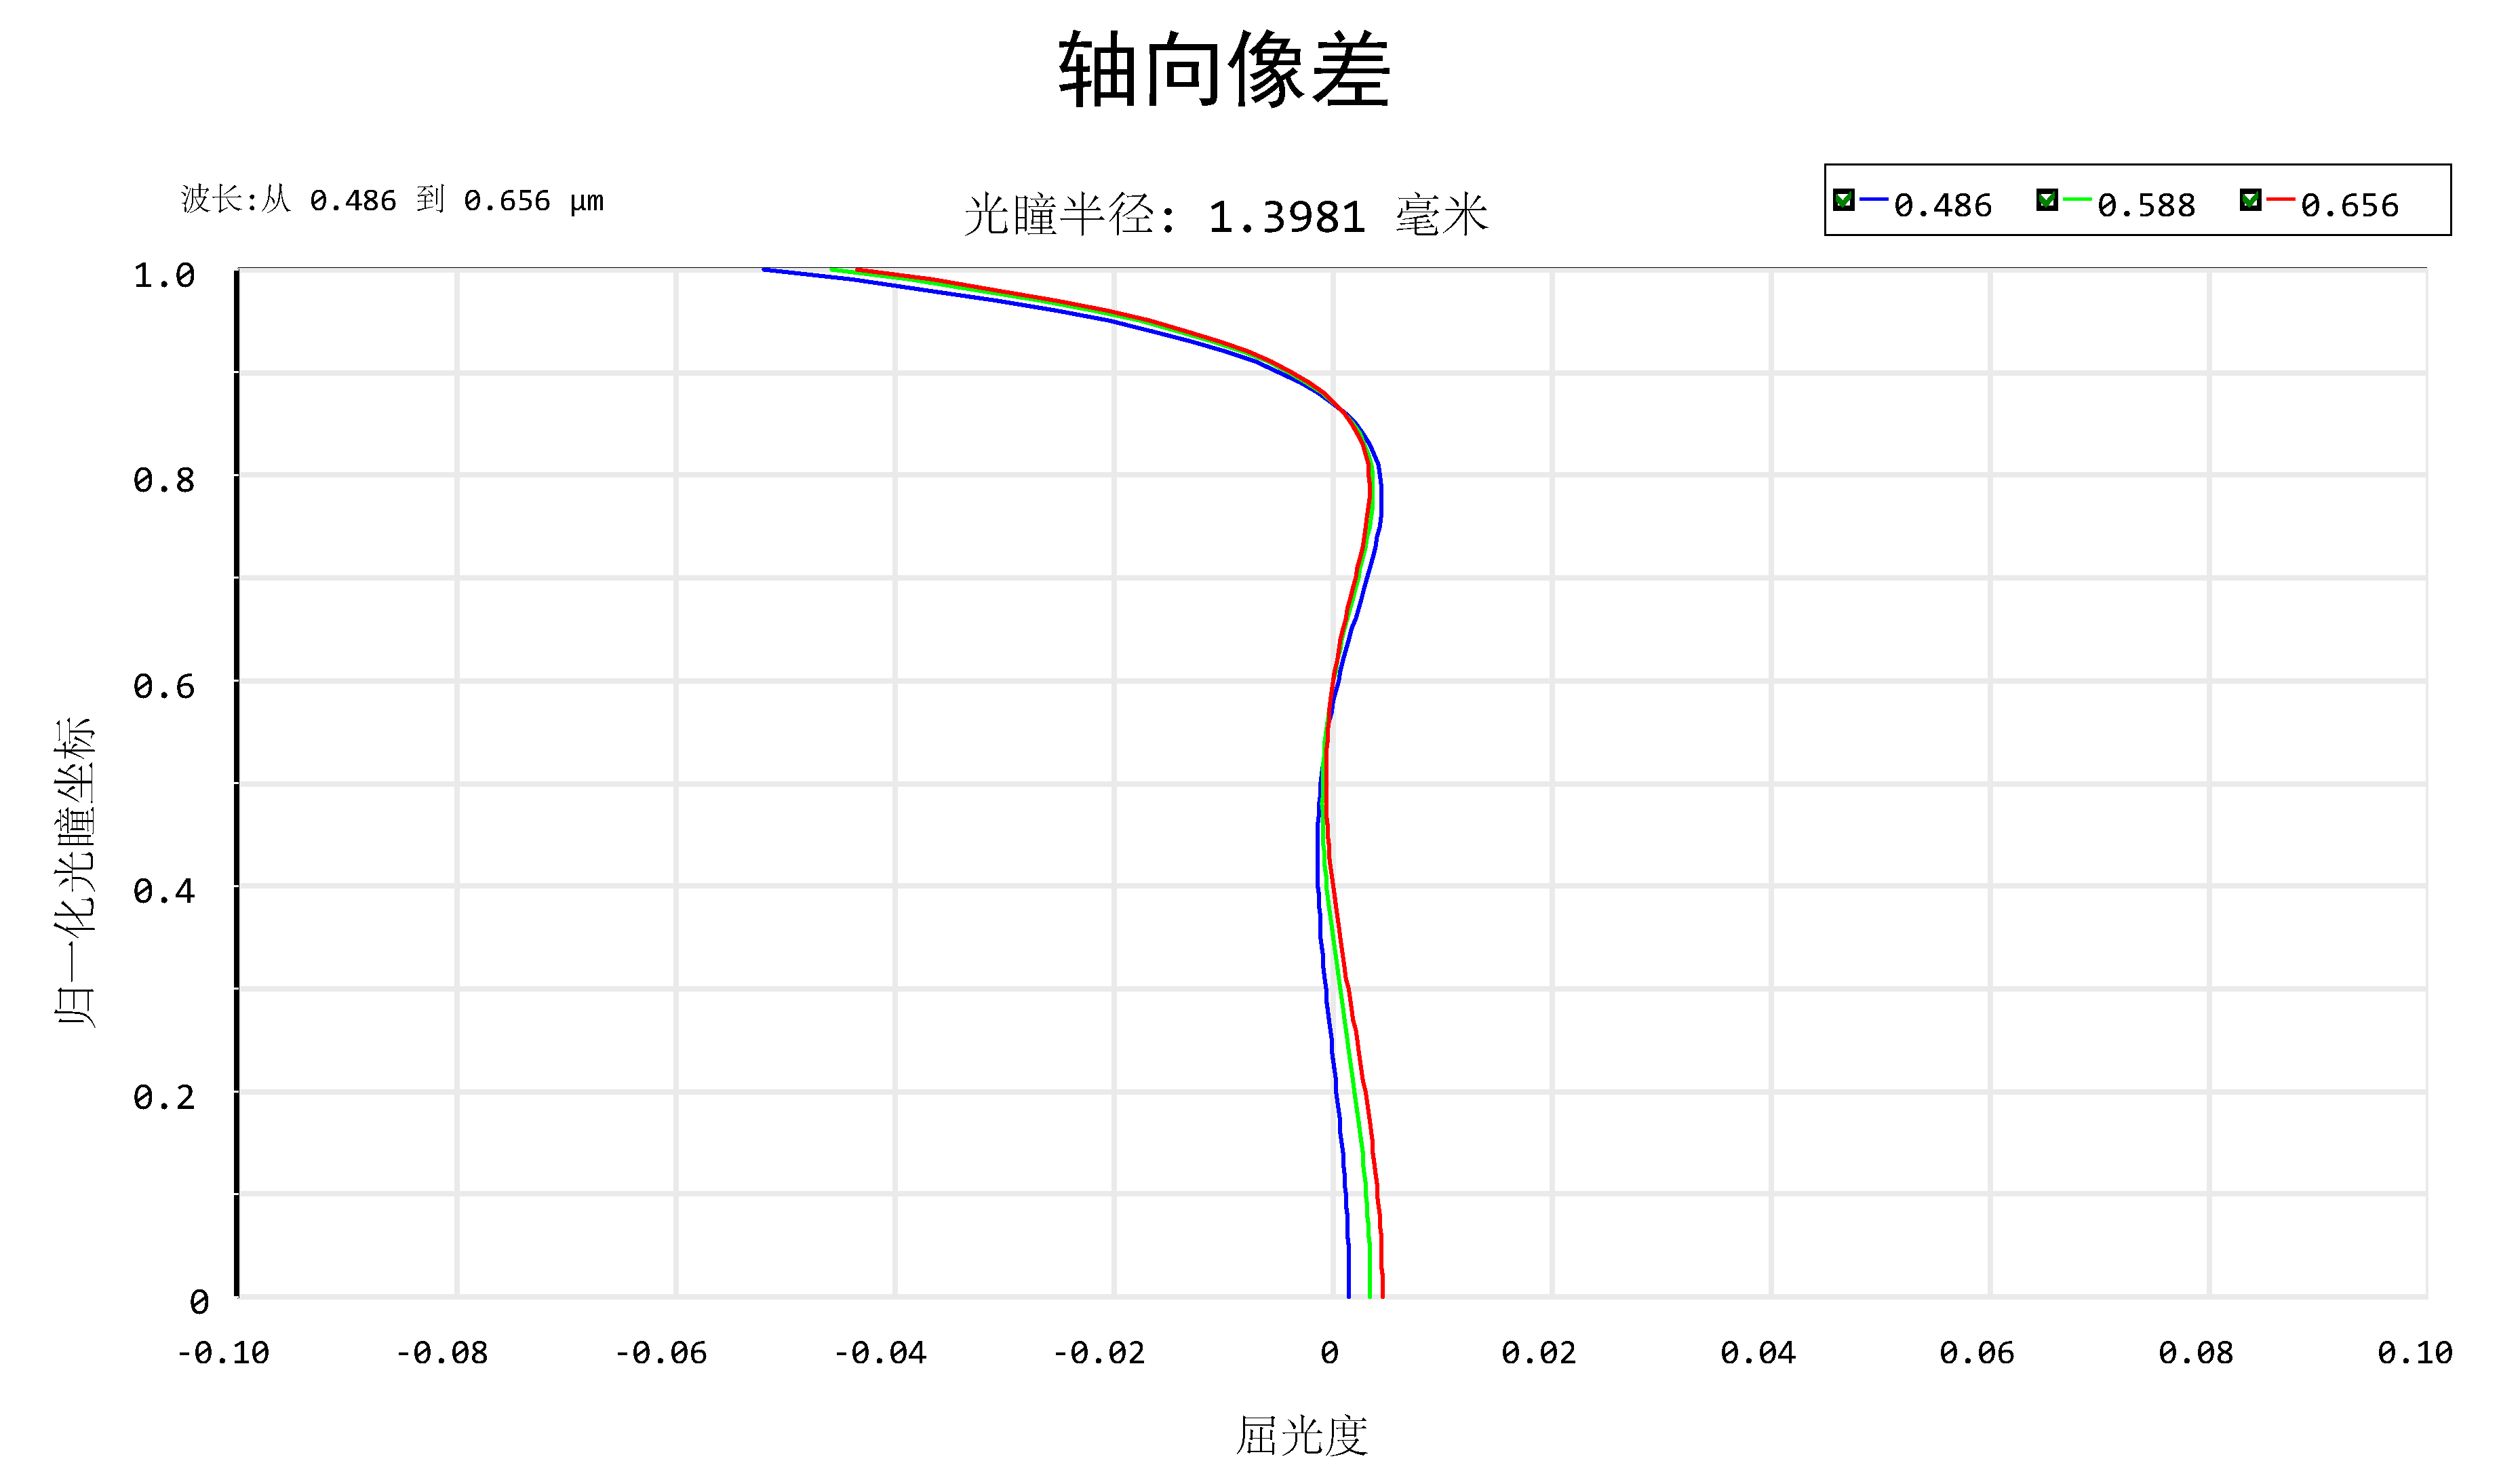
\includegraphics[width=\textwidth]{Fig/Fig-Obj-轴向像差.pdf}
        \caption{}
        \label{fig_obj_g}
    \end{subfigure}
    \bicaption{自研空气物镜的补充像差分析结果。(a)FFT PSF 截面图；(b)轴向像差曲线}
    {Supplementary aberration analysis of the self-designed air objective. (a) FFT PSF cross section; (b) longitudinal aberration curve}
    \label{fig_obj_psf_lsa}
\end{figure}


从设计结构上看，该物镜采用多片正负透镜组合，通过在前组与后组之间分配折射能力，实现对孔径、像方会聚以及像差校正的协同优化。表中所列的焦面附近关键面和光阑位置，可用于理解系统在数值孔径、工作距离与像场控制之间的折中关系。虽然该处方仍属于用于系统验证的简化模型，但其已经能够反映自研物镜在大视场条件下的实际设计自由度与加工约束。

图~\ref{fig_obj_psf_lsa} 进一步给出了自研空气物镜的 FFT PSF 截面图与轴向像差曲线。FFT PSF 截面能够直观反映焦点附近能量集中程度及像斑对称性，而轴向像差曲线则用于评估不同孔径区域光线在像方的会聚一致性。两者结合表明，该自研物镜在当前设计参数下能够维持较好的轴向成像一致性，并为正文中关于其大视场成像潜力的讨论提供补充依据。



\stepcounter{app}
\setcounter{app_fig}{1}
\setcounter{app_tab}{1}
\setcounter{equation}{0}

\chapter{超短脉冲压缩与表征补充分析}
\section{自相干仪测量原理与预实验条件}
在开展脉冲宽度表征之前，首先需要对待测激光的平均输出功率以及脉冲稳定性(pulse-to-pulse stability)进行标定，测试结果如图~\ref{fig41-42} 所示。该步骤对于后续自相干测量尤为关键，因为本文所采用的探测机制基于双光子吸收(Two-Photon Absorption, TPA)效应，而 TPA 属于典型的非线性光学过程，其信号强度与入射光强的平方成正比，即

\begin{equation}
    I_{\mathrm{TPA}} \propto I^2
\end{equation}

这意味着一旦激光器相邻脉冲之间存在明显的能量波动，非线性探测过程会进一步放大这种波动，从而在自相干信号中引入较大的幅值噪声，最终降低脉冲宽度测量的准确性与重复性。因此，稳定的输出功率和良好的脉冲间一致性是获得高信噪比自相干曲线的前提条件。

\begin{figure}[htbp]
    \centering
    \begin{subfigure}[b]{0.52\textwidth}
        \centering
        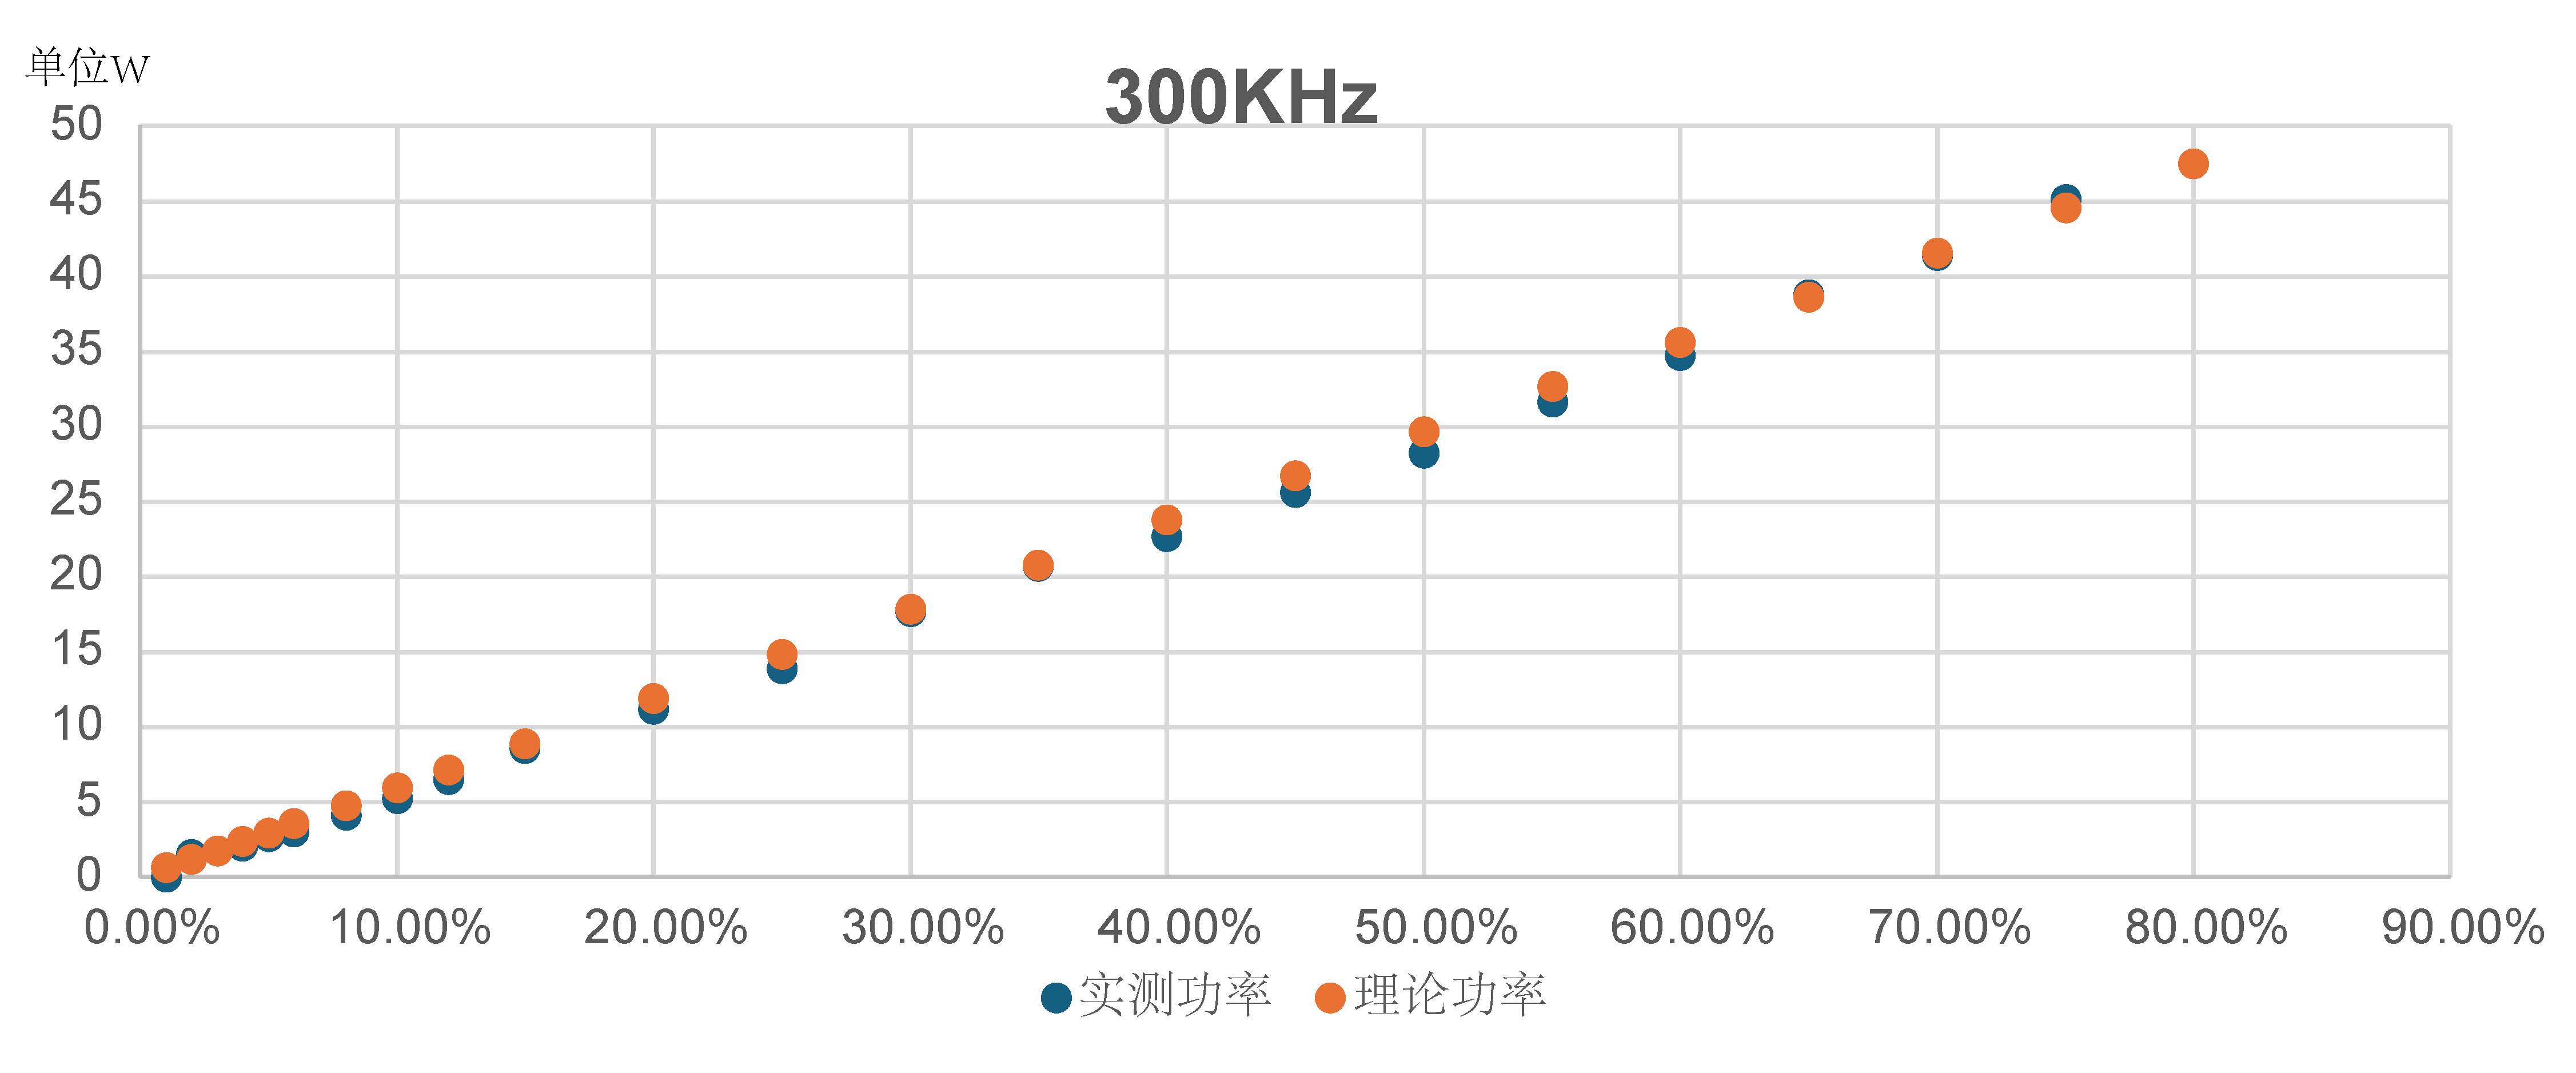
\includegraphics[width=\textwidth]{Fig/Fig41.pdf}
        \caption{}
        \label{fig41}
    \end{subfigure}
    \begin{subfigure}[b]{0.37\textwidth}
        \centering
        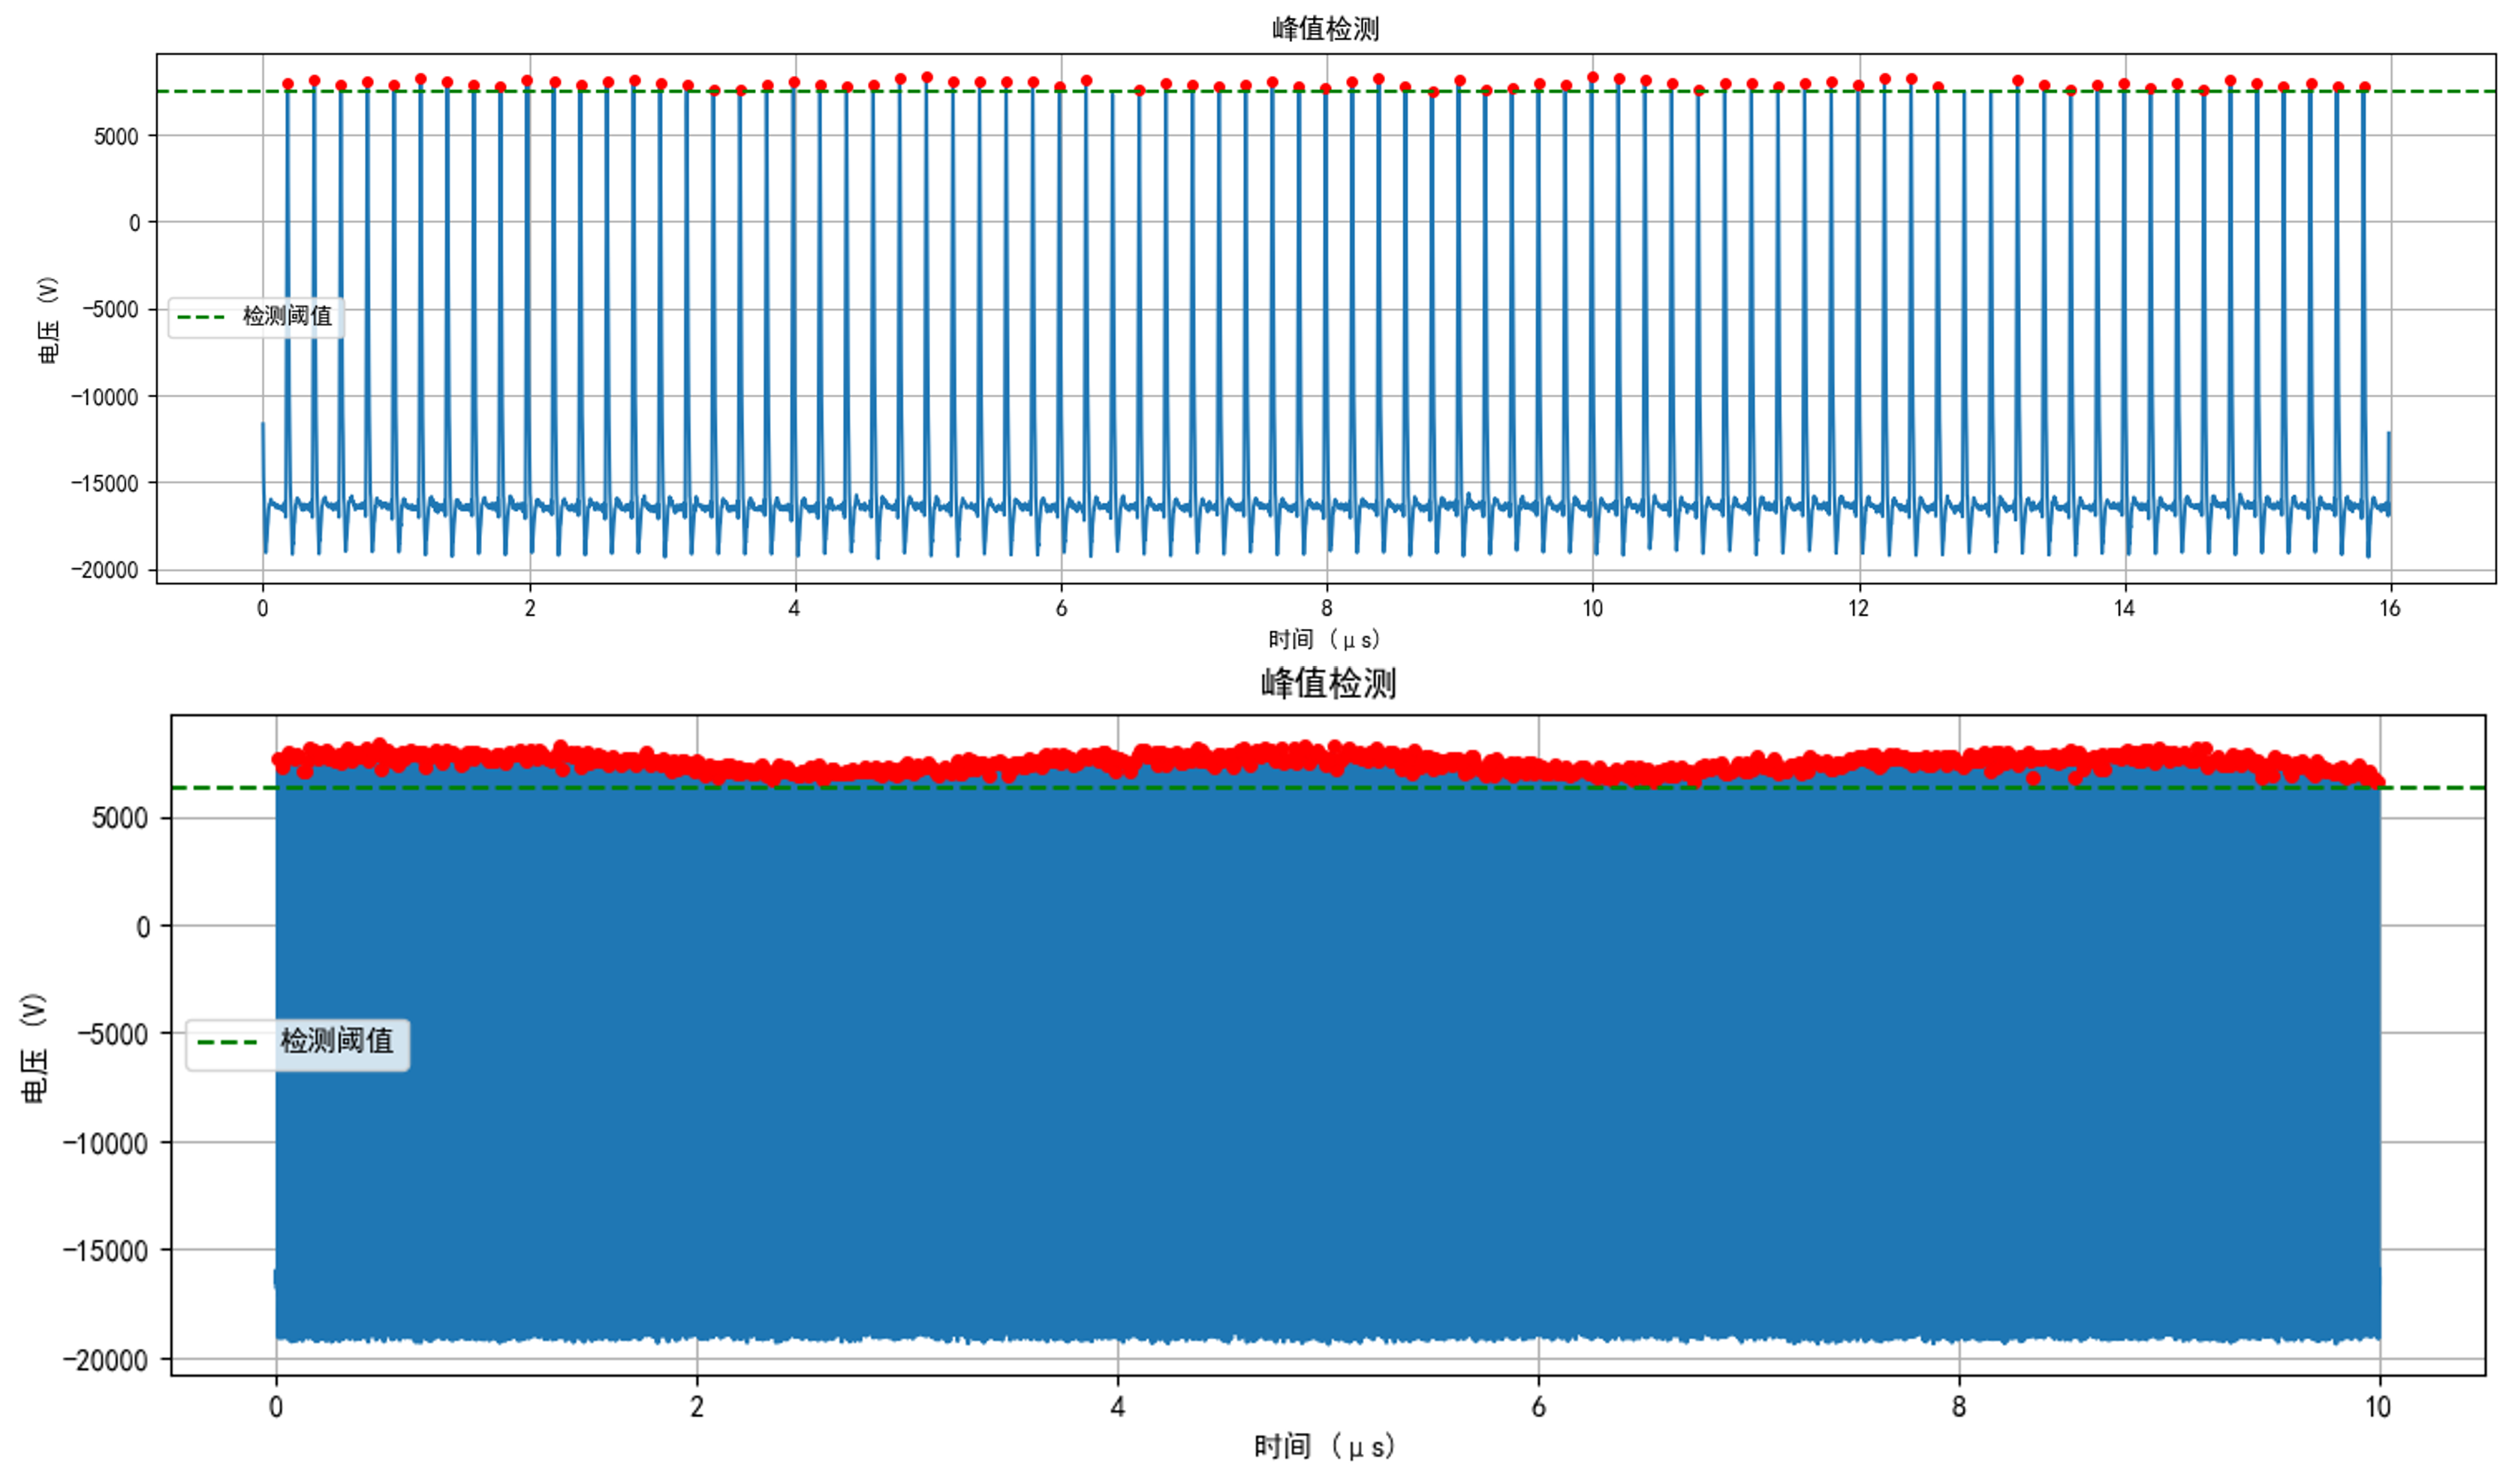
\includegraphics[width=\textwidth]{Fig/Fig42.png}
        \caption{}
        \label{fig42}
    \end{subfigure}
    \bicaption{待测激光的平均功率与脉冲稳定性标定结果。(a) 待测激光平均功率标定结果；(b) 待测激光脉冲稳定性标定结果}{Calibration results of the average power and pulse stability of the laser under test. (a) Average-power calibration; (b) pulse-stability characterization}
    \label{fig41-42}
\end{figure}



\subsection{干涉自相关的数学模型与峰背比}\label{app:auto_math}

在基于双光子吸收的干涉自相关测量中，光电二极管(Photodiode, PD)输出的光电流与入射到探测器表面的总光强平方成正比。由于探测器的响应时间远大于飞秒脉冲本身的持续时间，实验系统实际记录的是光电流的时间积分结果。因此，干涉自相关信号强度 $I_{AC}(\tau)$ 可表示为
\begin{equation}
    I_{AC}(\tau)=\int_{-\infty}^{\infty}|[E(t)+E(t-\tau)]^{2}|^{2}dt
\end{equation}

其中，$E(t)$ 为脉冲复电场振幅，$\tau$ 为移动臂引入的时间延迟。将上式展开后，可得
\begin{align}
    I_{AC}(\tau)=&\int_{-\infty}^{\infty}[I(t)^{2}+I(t-\tau)^{2}]dt\\ \notag
    &+4\int_{-\infty}^{\infty}[I(t)+I(t-\tau)Re\{E(t)E^{*}(t-\tau)\}]dt\\ \notag
    &+2\int_{-\infty}^{\infty}Re\{E(t)^{2}E^{*}(t-\tau)^{2}\}dt\\ \notag
    &+4\int_{-\infty}^{\infty}I(t)I(t-\tau)dt
\end{align}

上述表达式中包含四类主要成分：
\begin{enumerate}
    \item 第一项对应恒定背景信号；
    \item 第二项为基频光的干涉项，在自相关曲线中心区域形成与载波频率对应的快速干涉条纹；
    \item 第三项为二次谐波分量对应的干涉项；
    \item 第四项为纯强度自相关(intensity autocorrelation)项，反映脉冲包络的重叠程度。
\end{enumerate}

图~\ref{fig42.56}(\subref{fig42.5}) 给出了理想干涉自相关信号的典型特征。在理想相位匹配以及分光均衡的条件下，当 $\tau=0$ 时，两束脉冲在时间上完全重合，干涉信号达到最大值；而当 $\tau \rightarrow \infty$ 时，两束脉冲彼此分离，仅保留恒定背景。此时自相关曲线的峰值与背景之比理论上为 $8:1$。实际实验中，由于分光比误差、光束准直偏差以及器件装调误差等因素的影响，该峰背比通常略低于理论值，一般可达到约 $7:1$。因此，峰背比不仅是判断系统干涉质量的重要指标，也可作为评价光路重合程度与装调精度的依据。


\subsection{脉冲宽度的解算(去相关因子)}\label{app:auto_deconv}

由自相关曲线直接测得的半高全宽(Full Width at Half Maximum, FWHM)，记为 $\tau_{ac}$，并不等于脉冲真实宽度 $\tau_{pulse}$。要由自相关宽度反推出实际脉冲宽度，还需要结合脉冲的包络形状引入相应的去相关因子。对于干涉自相关曲线的上包络，其换算关系通常为：

若脉冲包络近似为高斯型(Gaussian)，则有
\[
\tau_{pulse}=\tau_{ac}/1.7
\]

若脉冲包络近似为双曲正割平方型($\mathrm{sech}^2$)，则有
\[
\tau_{pulse}=\tau_{ac}/1.9
\]

因此，在利用自相关法计算脉冲宽度时，必须首先对脉冲形状作出合理假设，否则将给最终结果带来系统性误差。



\subsection{脉冲啁啾(Chirp)现象的识别与分析}\label{app:auto_chirp}

在超快光学系统中，飞秒脉冲在光学介质中传播时不可避免地会受到群速度色散以及更高阶色散的影响，从而导致脉冲时域展宽并产生啁啾(chirp)。因此，在评估脉冲压缩系统性能时，干涉自相关仪不仅可用于测量脉冲宽度，还可作为判断残余啁啾的重要诊断手段。

当脉冲具有明显啁啾时，其时间持续宽度会显著增大，而相干长度相对较短。此时在干涉自相关曲线上，常出现``宽底座叠加窄尖峰''的特征，如图~\ref{fig42.56}(\subref{fig42.6}) 所示。具体而言，在延迟时间较大的区域，两束脉冲虽然在时间上仍可能存在部分重叠，但由于瞬时频率失配，相位相关性显著下降，干涉条纹逐渐消失，曲线两侧仅保留较宽的强度自相关包络；而在 $\tau \approx 0$ 的中心区域，由于两束光在时间与相位上仍保持较强相干性，因此会形成一个窄而尖锐的干涉峰。

图~\ref{fig42.56}(\subref{fig42.6}) 所示的这种``宽底座 $+$ 窄尖峰''结构正是严重啁啾脉冲的典型表征。该结果说明，若直接以整条干涉自相关曲线的半高全宽来估算脉冲宽度，往往会导致对实际脉冲时宽的误判。针对这类信号，更合理的做法是先通过频域滤波或包络提取方法去除高频干涉条纹，仅保留强度自相关包络，再结合去相关因子对脉冲宽度进行计算。由此可见，干涉自相关曲线不仅反映脉冲时宽信息，也能够直观揭示脉冲是否存在显著残余啁啾。

\begin{figure}[htbp]
    \centering
    \begin{subfigure}[b]{0.45\textwidth}
        \centering
        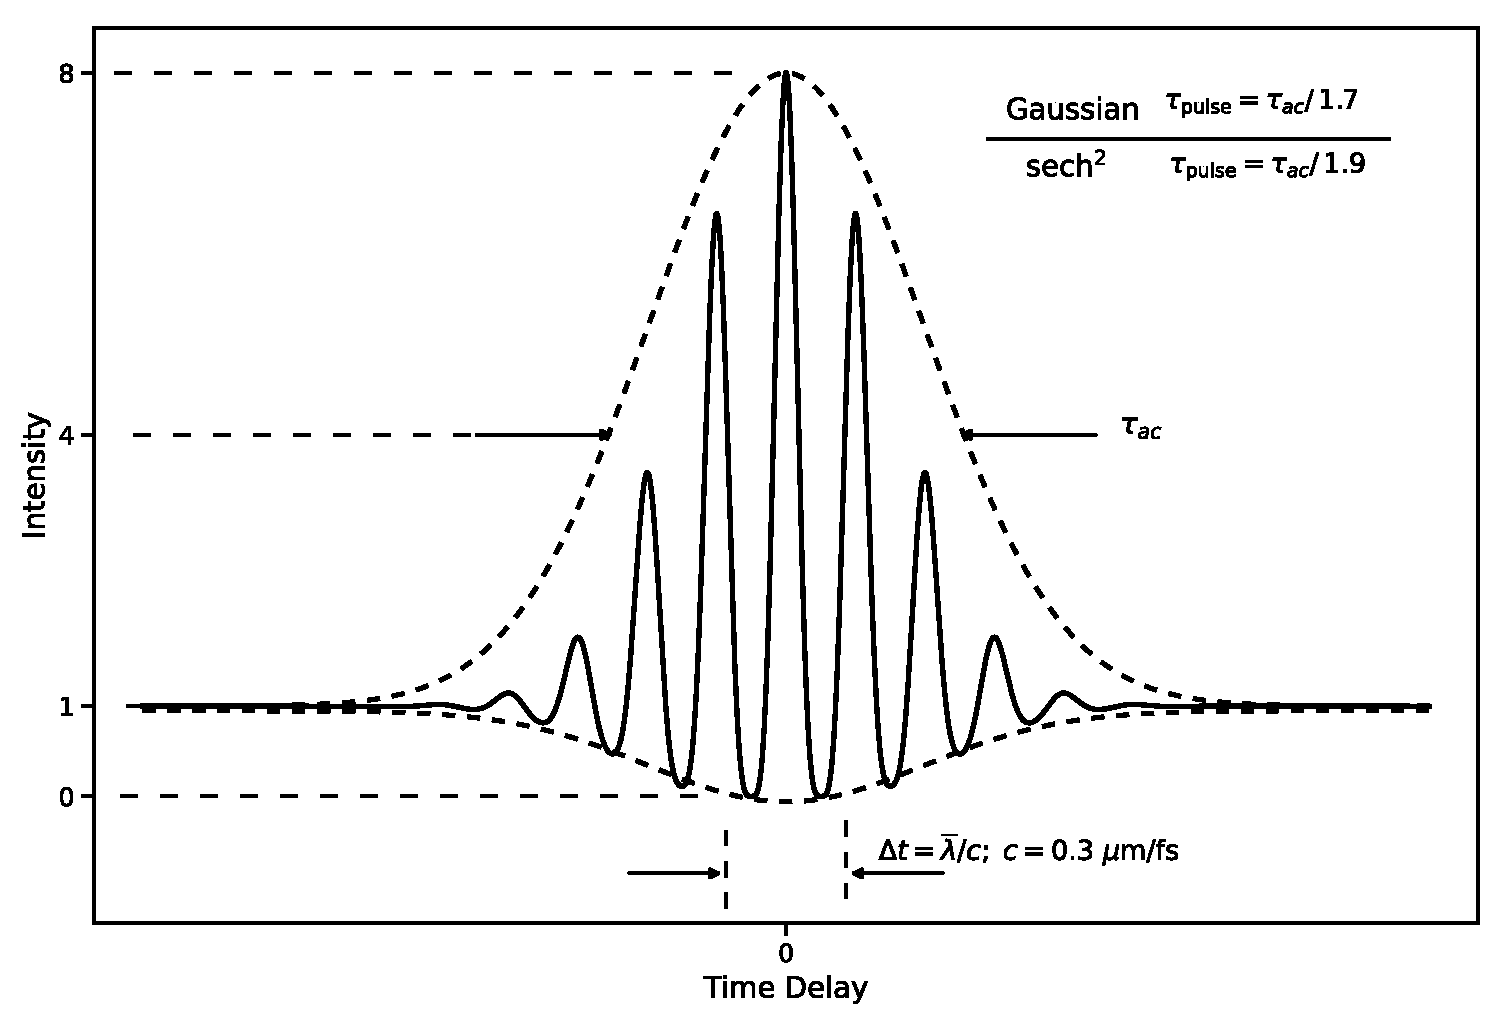
\includegraphics[width=\textwidth]{Fig/Fig42.5.pdf}
        \caption{}
        \label{fig42.5}
    \end{subfigure}
    \begin{subfigure}[b]{0.45\textwidth}
        \centering
        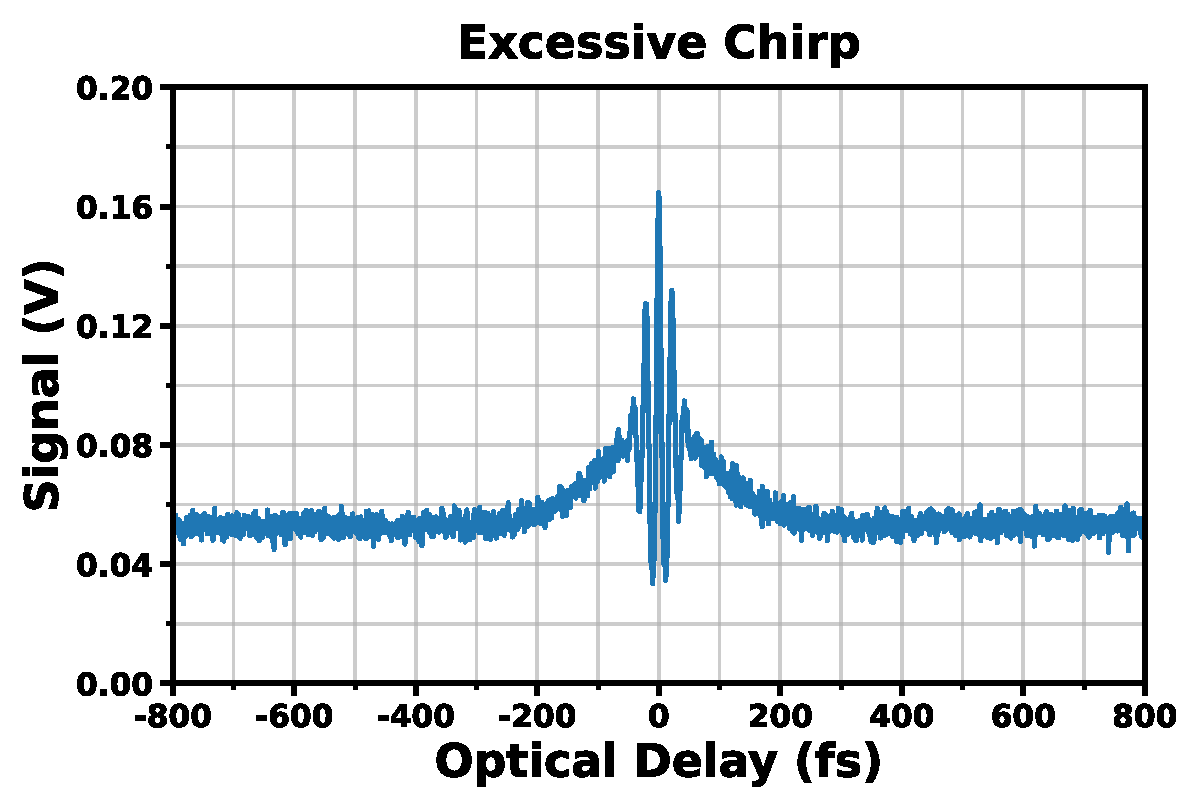
\includegraphics[width=\textwidth]{Fig/Fig42.6.pdf}
        \caption{}
        \label{fig42.6}
    \end{subfigure}
    \bicaption{自相干干涉信号特征及啁啾脉冲分析示意图。(a) 强度自相关仪中的干涉信号峰值背景比；(b) 严重啁啾飞秒脉冲的干涉自相关曲线\cite{thorlabs}}{Characteristic interferometric autocorrelation signals and analysis of chirped pulses. (a) Peak-to-background ratio of the interference signal in an intensity autocorrelator; (b) interferometric autocorrelation trace of a strongly chirped femtosecond pulse\cite{thorlabs}}
    \label{fig42.56}
\end{figure}



\section{多通腔脉冲压缩补充仿真结果}

% 为补充说明 MPC 脉冲压缩中的非线性展宽机理及色散敏感性，本文在附录中进一步给出了腔镜本征模覆盖、纯 SPM 频谱展宽以及不同阶色散作用下脉冲时域展宽的补充仿真结果。

% \begin{figure}[htbp]
%     \centering
%     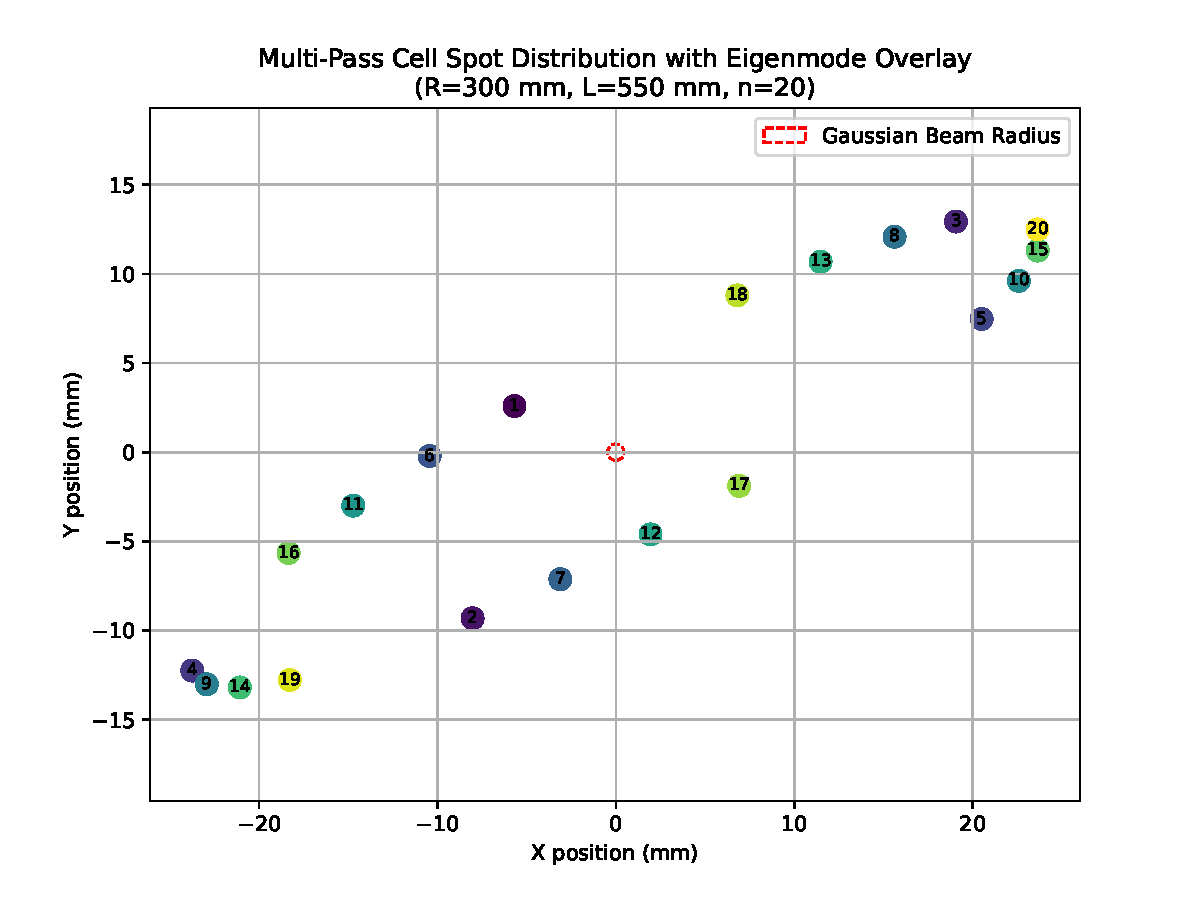
\includegraphics[width=0.75\textwidth]{Fig/MPC-Figure_5.pdf}
%     \bicaption{MPC 腔镜上的反射点分布及本征模覆盖示意图}
%     {Reflection-spot distribution on the MPC mirrors with eigenmode overlay}
%     \label{fig:mpc_appendix_mode}
% \end{figure}

% 图~\ref{fig:mpc_appendix_mode} 给出了 MPC 腔镜上的反射点分布及其与高斯本征模半径的对照结果，可用于辅助判断给定腔长、曲率半径和反射次数下的光斑利用率与模式匹配情况。

\begin{figure}[htbp]
    \centering
    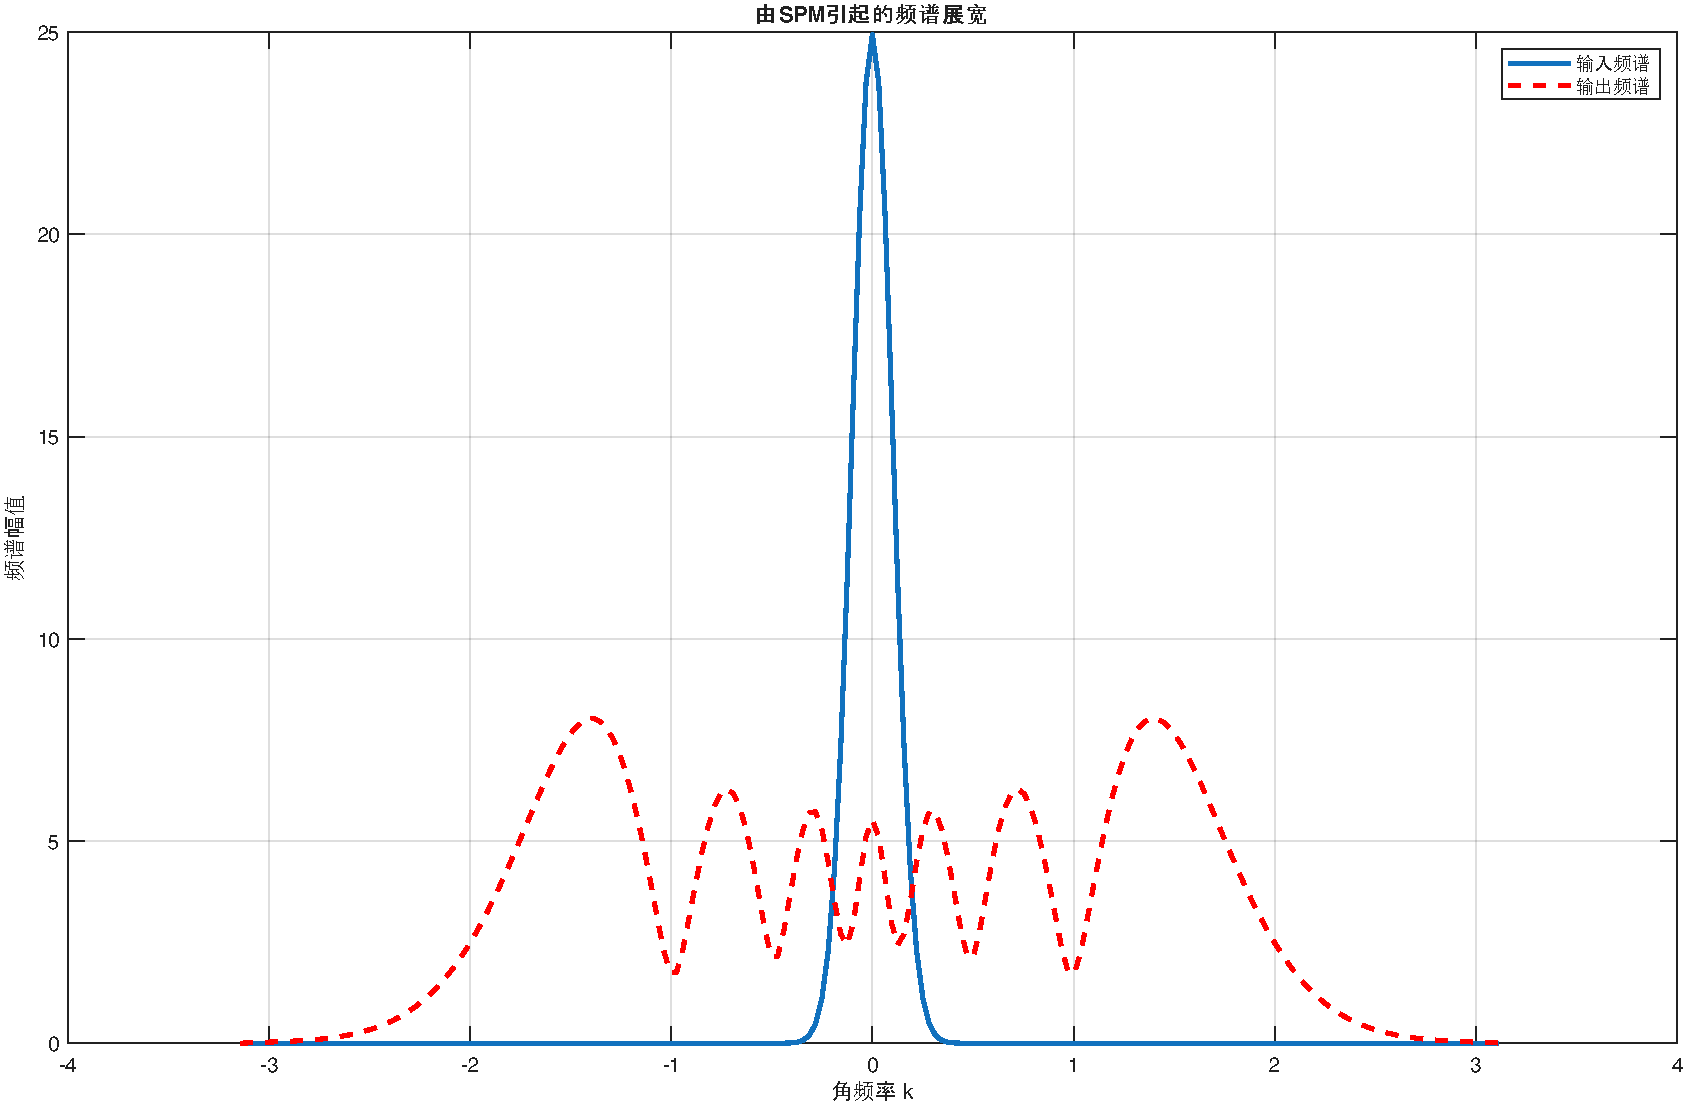
\includegraphics[width=0.70\textwidth]{Fig/MPC-Figure_6.pdf}
    \bicaption{仅考虑自相位调制时的频谱展宽示意图}
    {Spectral broadening induced by self-phase modulation only}
    \label{fig:mpc_appendix_spm}
\end{figure}

图~\ref{fig:mpc_appendix_spm} 展示了在仅考虑自相位调制效应、忽略色散项的条件下，脉冲频谱随传播距离的展宽趋势。该结果主要用于说明 SPM 是 MPC 光谱展宽的主要驱动机制之一，而非作为最终压缩结果的定量依据。

图~\ref{fig:mpc_appendix_dispersion} 比较了二阶、三阶和四阶色散对 5 fs 与 10 fs 高斯脉冲时域形状的影响。结果表明，脉宽越短，对高阶色散越敏感。这也说明在实际脉冲压缩设计中，仅依赖二阶色散补偿通常只能得到近似最优结果，而更高阶色散项会进一步影响压缩极限和旁瓣结构。

\begin{figure}[htbp]
    \centering
    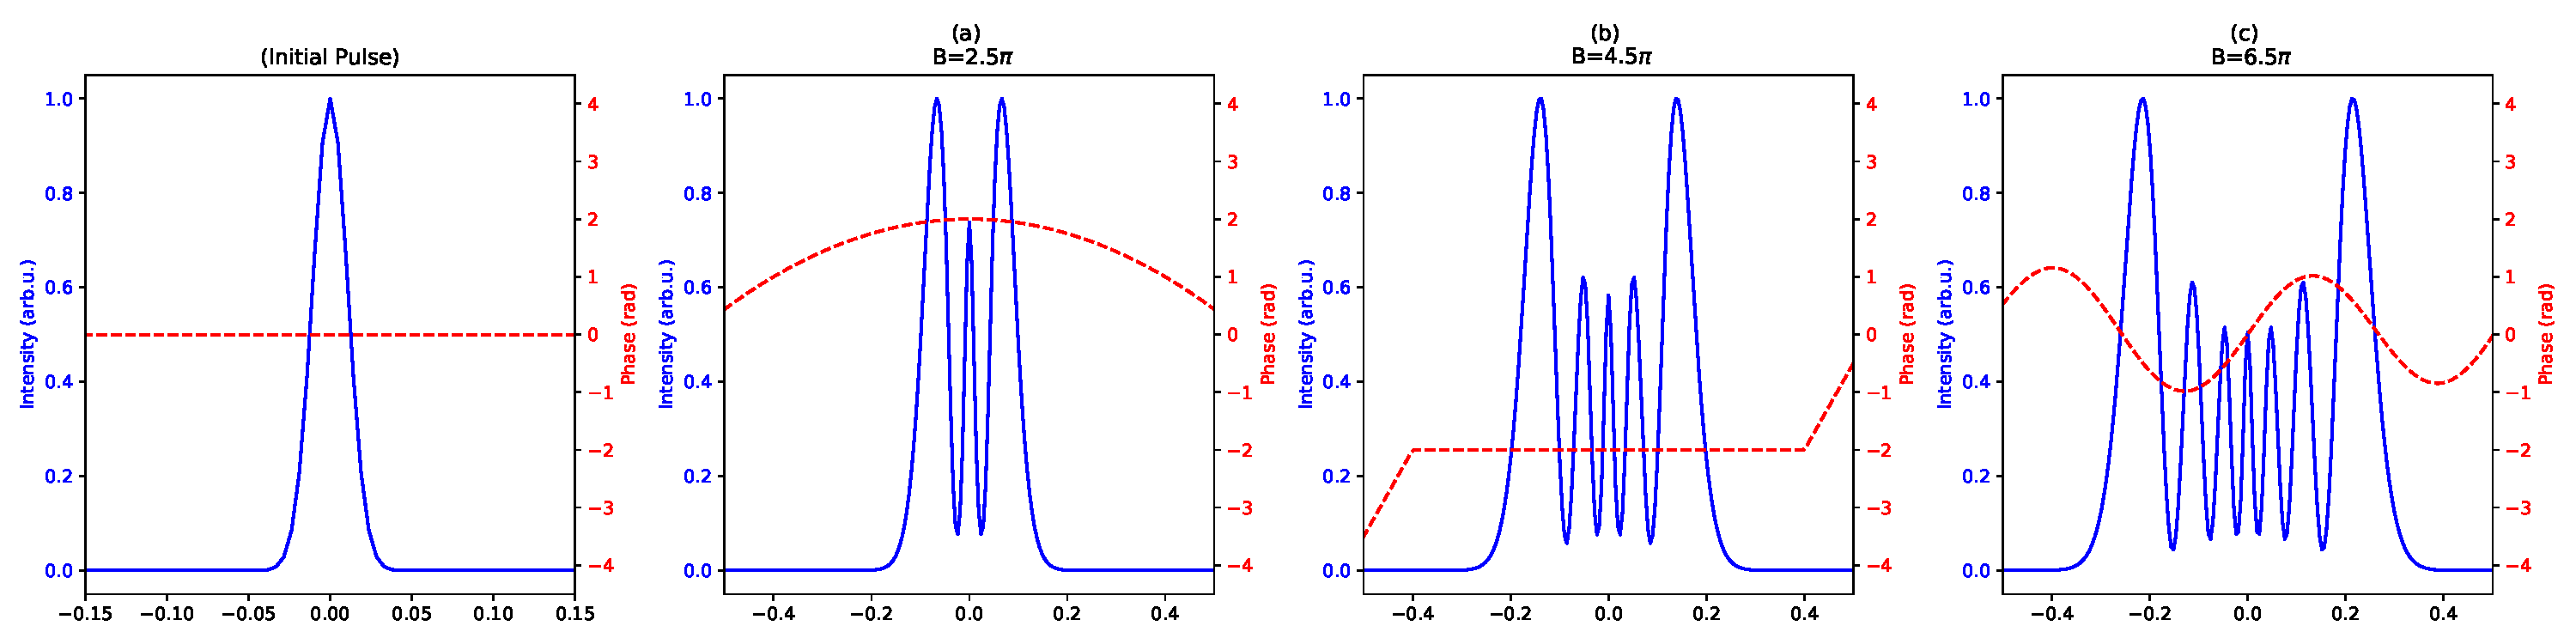
\includegraphics[width=0.98\textwidth]{Fig/MPC-Figure_2.pdf}
    \bicaption{不同阶色散对超短高斯脉冲时域形状的影响}
    {Influence of different dispersion orders on ultrashort Gaussian pulses in the time domain}
    \label{fig:mpc_appendix_dispersion}
\end{figure}


=======
\centering
\caption{变色龙}
\label{tab:optical_prescription}
\begin{tabular}{|c|l|c|c|c|c|}
\hline
\multicolumn{2}{|c|}{Surface} & Radius (mm) & Thickness (mm) & Material & Semidiameter \\ \hline
Stop & Back aperture & Inf & -1.000 &  & 10 \\ \hline
2  &  & -14.773  & 13.669 & S-LAH58 & 11.27 \\
3  &  & 1572.581 & 12.899 & S-LAL21 & 18.118 \\
4  &  & -26.775  & 1.692  &         & 20.155 \\
5  &  & 240.655  & 7.464  & S-LAH59 & 21.497 \\
6  & Adj. gap      & -60.321 & 5.621  &         & 21.619 \\
7  &  & 47.162   & 10.302 & S-FPM2  & 18.679 \\
8  &  & -41.597  & 1.999  & S-NPH3  & 18.679 \\
9  &  & 84.414   & 0.5    &         & 16.643 \\
10 &  & 22.719   & 8.777  & S-LAH58 & 16.090 \\
11 &  & 45.328   & 2.194  &         & 13.93 \\
12 & Working dist.& Inf    & 20.006 &         & 13.752 \\
13 & Coverslip    & Inf    & 0.17   & BK-7    & 3.30 \\
14 &  & Inf       & 0.35   & SEAWATER & 3.30 \\
15 & Image plane  & Inf    &        & SEAWATER & 3.30 \\ \hline
\end{tabular}
\end{table}
}
>>>>>>> c4bb8a8e4d07c80bffd10fe9aeb672bafe56fbee




<<<<<<< HEAD
=======
\chapter{附录中的图表}\label{chap:app2}{
>>>>>>> c4bb8a8e4d07c80bffd10fe9aeb672bafe56fbee
\stepcounter{app}
\setcounter{app_fig}{1}
\setcounter{app_tab}{1}

<<<<<<< HEAD
\chapter{双椭圆级联等光程扫描结构的理论设计与仿真}\label{chap:app_double_ellipse}

本附录汇总了双椭圆级联扫描结构的理论推导、参数优化与 Zemax 仿真结果。该部分工作的主要定位是展示一种面向大视场、低畸变扫描的探索性结构设计，其结果目前仍以几何分析与光学仿真为主，尚未完成整机加工、装调与长期运行验证，因此不作为正文主线结论，而作为后续系统扩展方向的补充说明。

\section{传统扫描结构的局限性}\label{app:ellipse_1}


\begin{figure}[htbp]
    \centering
    \begin{subfigure}[b]{0.65\textwidth}
        \centering
        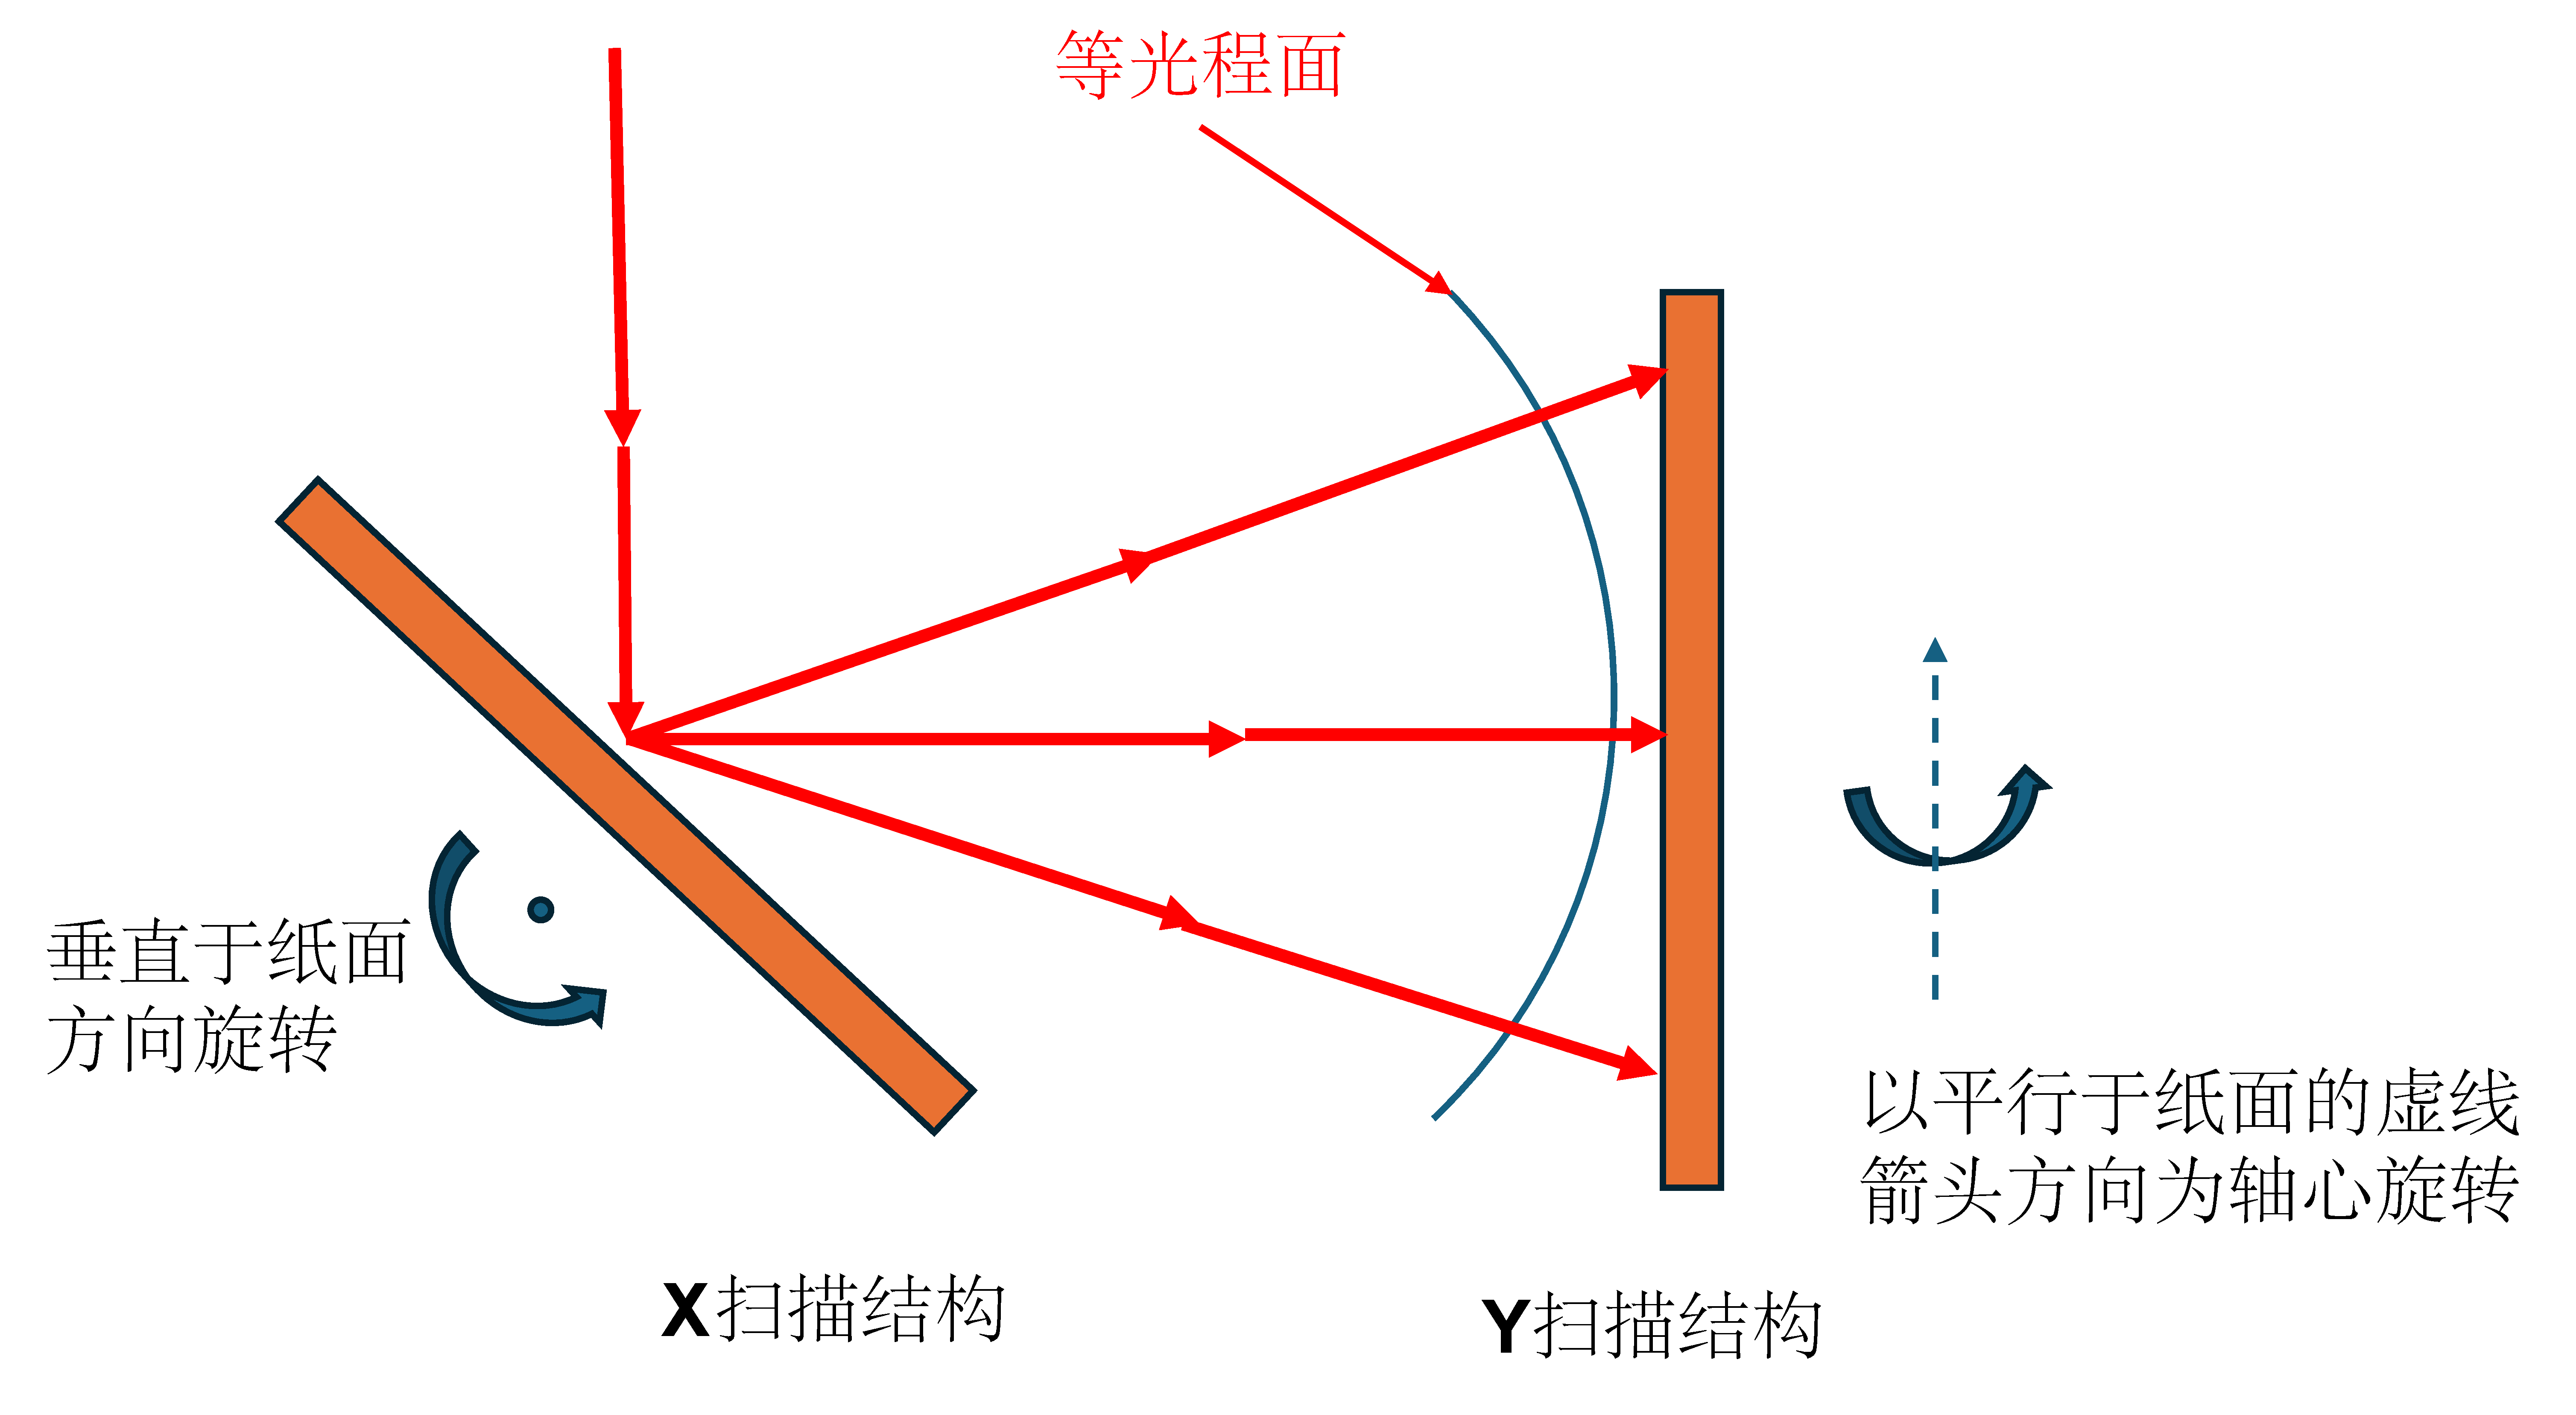
\includegraphics[width=\textwidth]{Fig/Fig58.pdf}
        \caption{}
        \label{fig58}
    \end{subfigure}

    \vspace{0.5em}

    \begin{subfigure}[b]{0.7\textwidth}
        \centering
        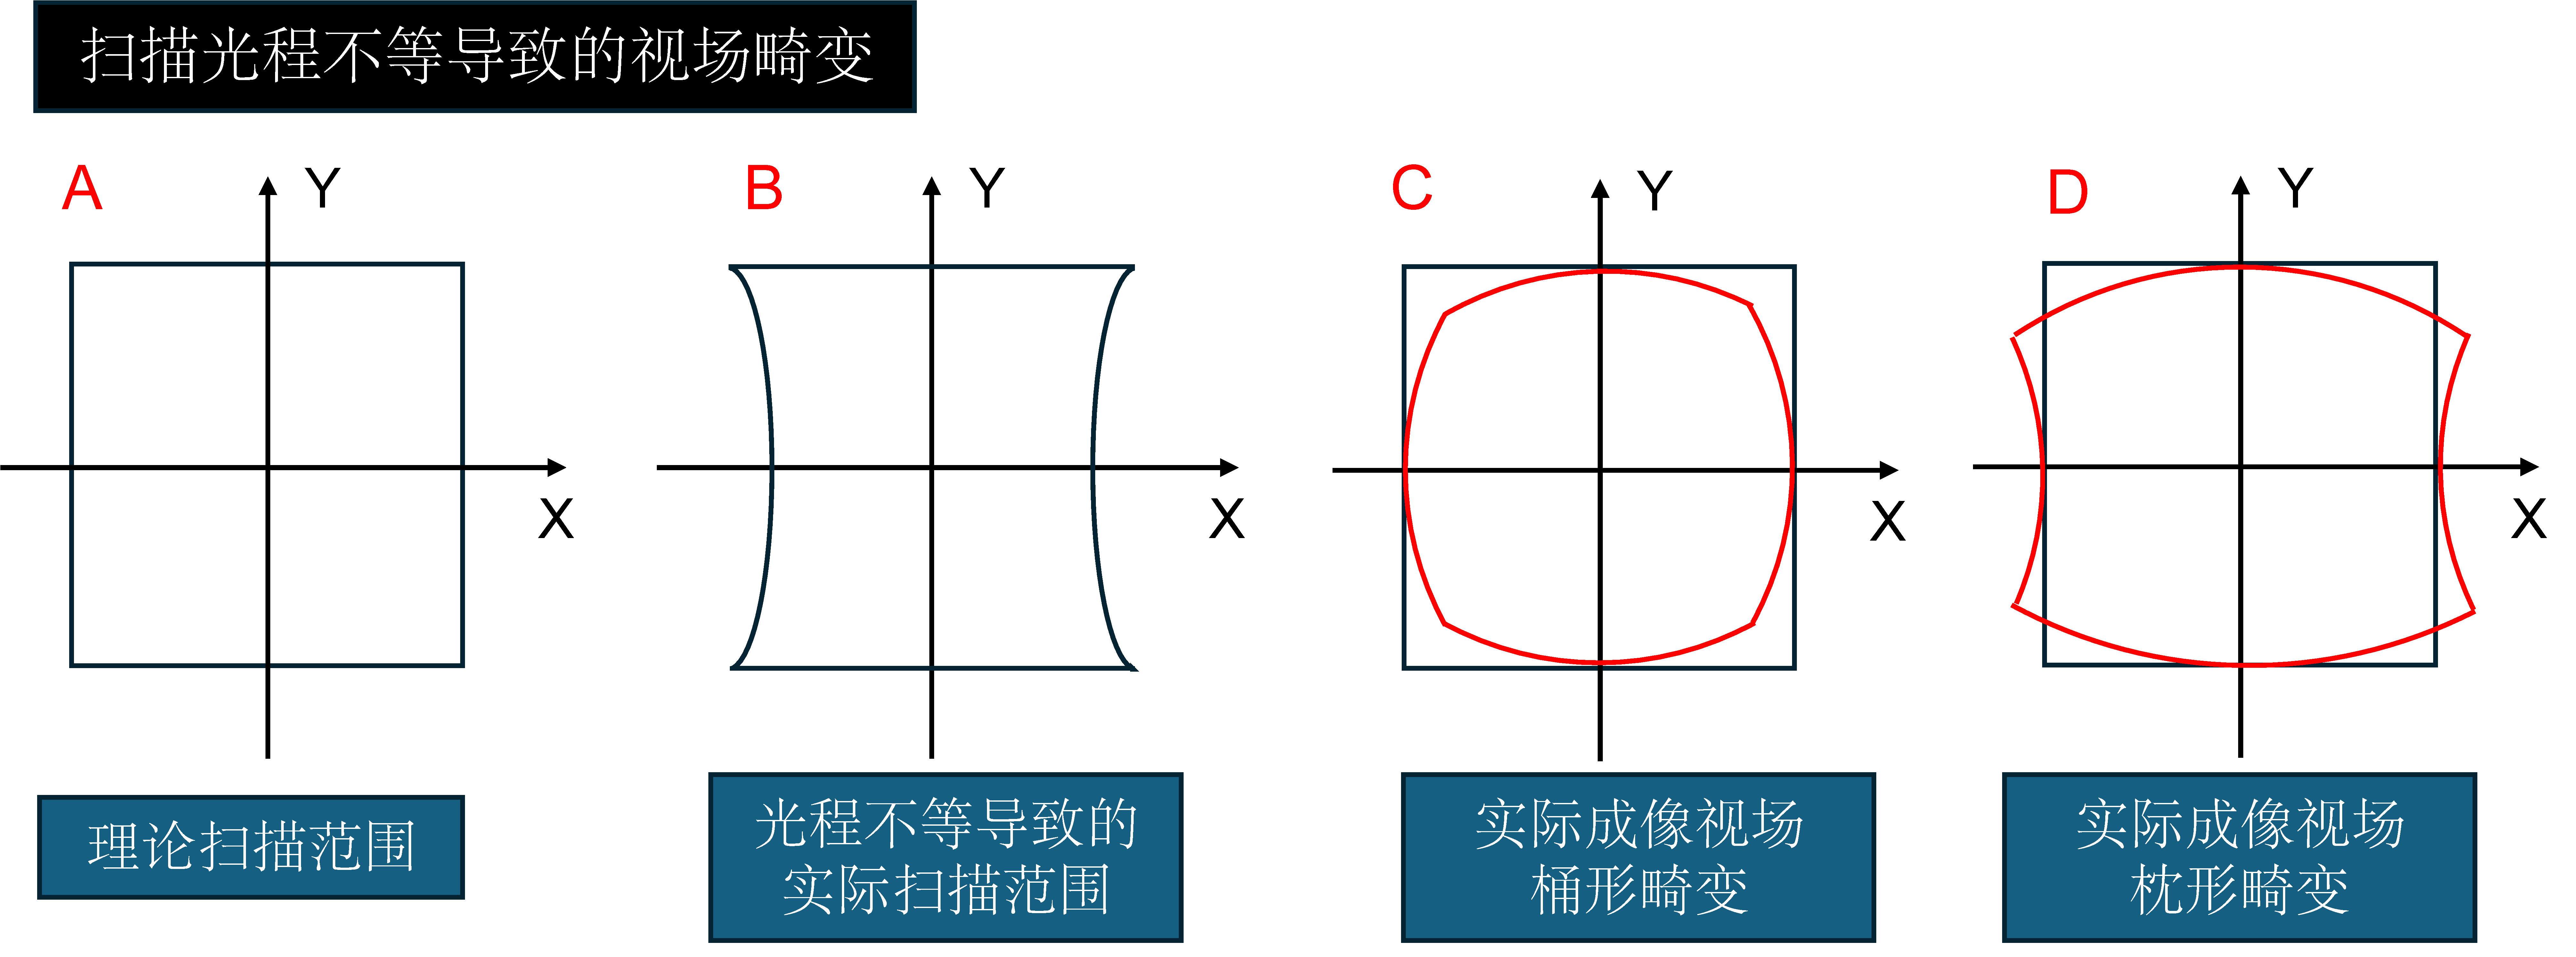
\includegraphics[width=\textwidth]{Fig/Fig60.pdf}
        \caption{}
        \label{fig60}
    \end{subfigure}

    \bicaption{扫描系统中的光程不等及其引起的视场畸变示意图。(a) 传统扫描结构中的光程不等与等光程面示意图；(b) 扫描光程不等导致的视场畸变(桶形畸变与枕形畸变)}{Schematic of unequal optical paths in scanning systems and the resulting field distortion. (a) Unequal optical paths and iso-optical-path surface in a conventional scanning structure; (b) field distortion caused by unequal scan paths, including barrel and pincushion distortion}
    \label{fig58-59}
\end{figure}

在传统光学扫描系统中，例如基于振镜或多面体扫描镜实现的扫描结构，扫描光束在空间中通常沿扇形轨迹偏转。由于不同扫描角对应的光线路径长度并不相同，系统中心视场与边缘视场之间往往存在显著的光程差。这种由扫描几何关系引起的光程不等，会进一步破坏理想成像条件，导致扫描视场中的几何映射关系发生偏离，最终表现为不同程度的视场畸变，如图~\ref{fig58-59}(\subref{fig58}) 所示。

相较于理想的线性扫描结果，实际系统中常见的畸变形式主要包括桶形畸变和枕形畸变，如图~\ref{fig58-59}(\subref{fig60}) 所示。前者表现为图像边缘向外鼓出，后者则表现为图像边缘向内收缩。无论是哪一种畸变，本质上都反映了扫描角、成像位置与实际光程之间的不一致。这种非理想效应不仅会降低边缘区域的成像质量，还会对空间定位精度、扫描均匀性以及后续图像重建带来不利影响。因此，对于大视场、高精度的扫描成像系统而言，如何在扩大扫描范围的同时保证各扫描位置的等效光程一致，是系统设计中需要重点解决的问题。


\section{椭圆等光程扫描原理}\label{app:ellipse_2}

为减小传统扫描结构中由光程不等引起的视场畸变，本文引入了基于椭圆几何光学特性的等光程扫描方案。椭圆作为一种具有特殊反射性质的二次曲线，其最重要的光学特征之一在于：从一个焦点出发并经椭圆反射面的任意光线，最终均会汇聚到另一个焦点，且从一个焦点经椭圆面到另一焦点的总光程保持恒定。正是这一性质，为实现大视场下的等光程扫描提供了可行的理论基础。



\begin{figure}[htbp]
    \centering
    \begin{subfigure}[b]{0.44\textwidth}
        \centering
        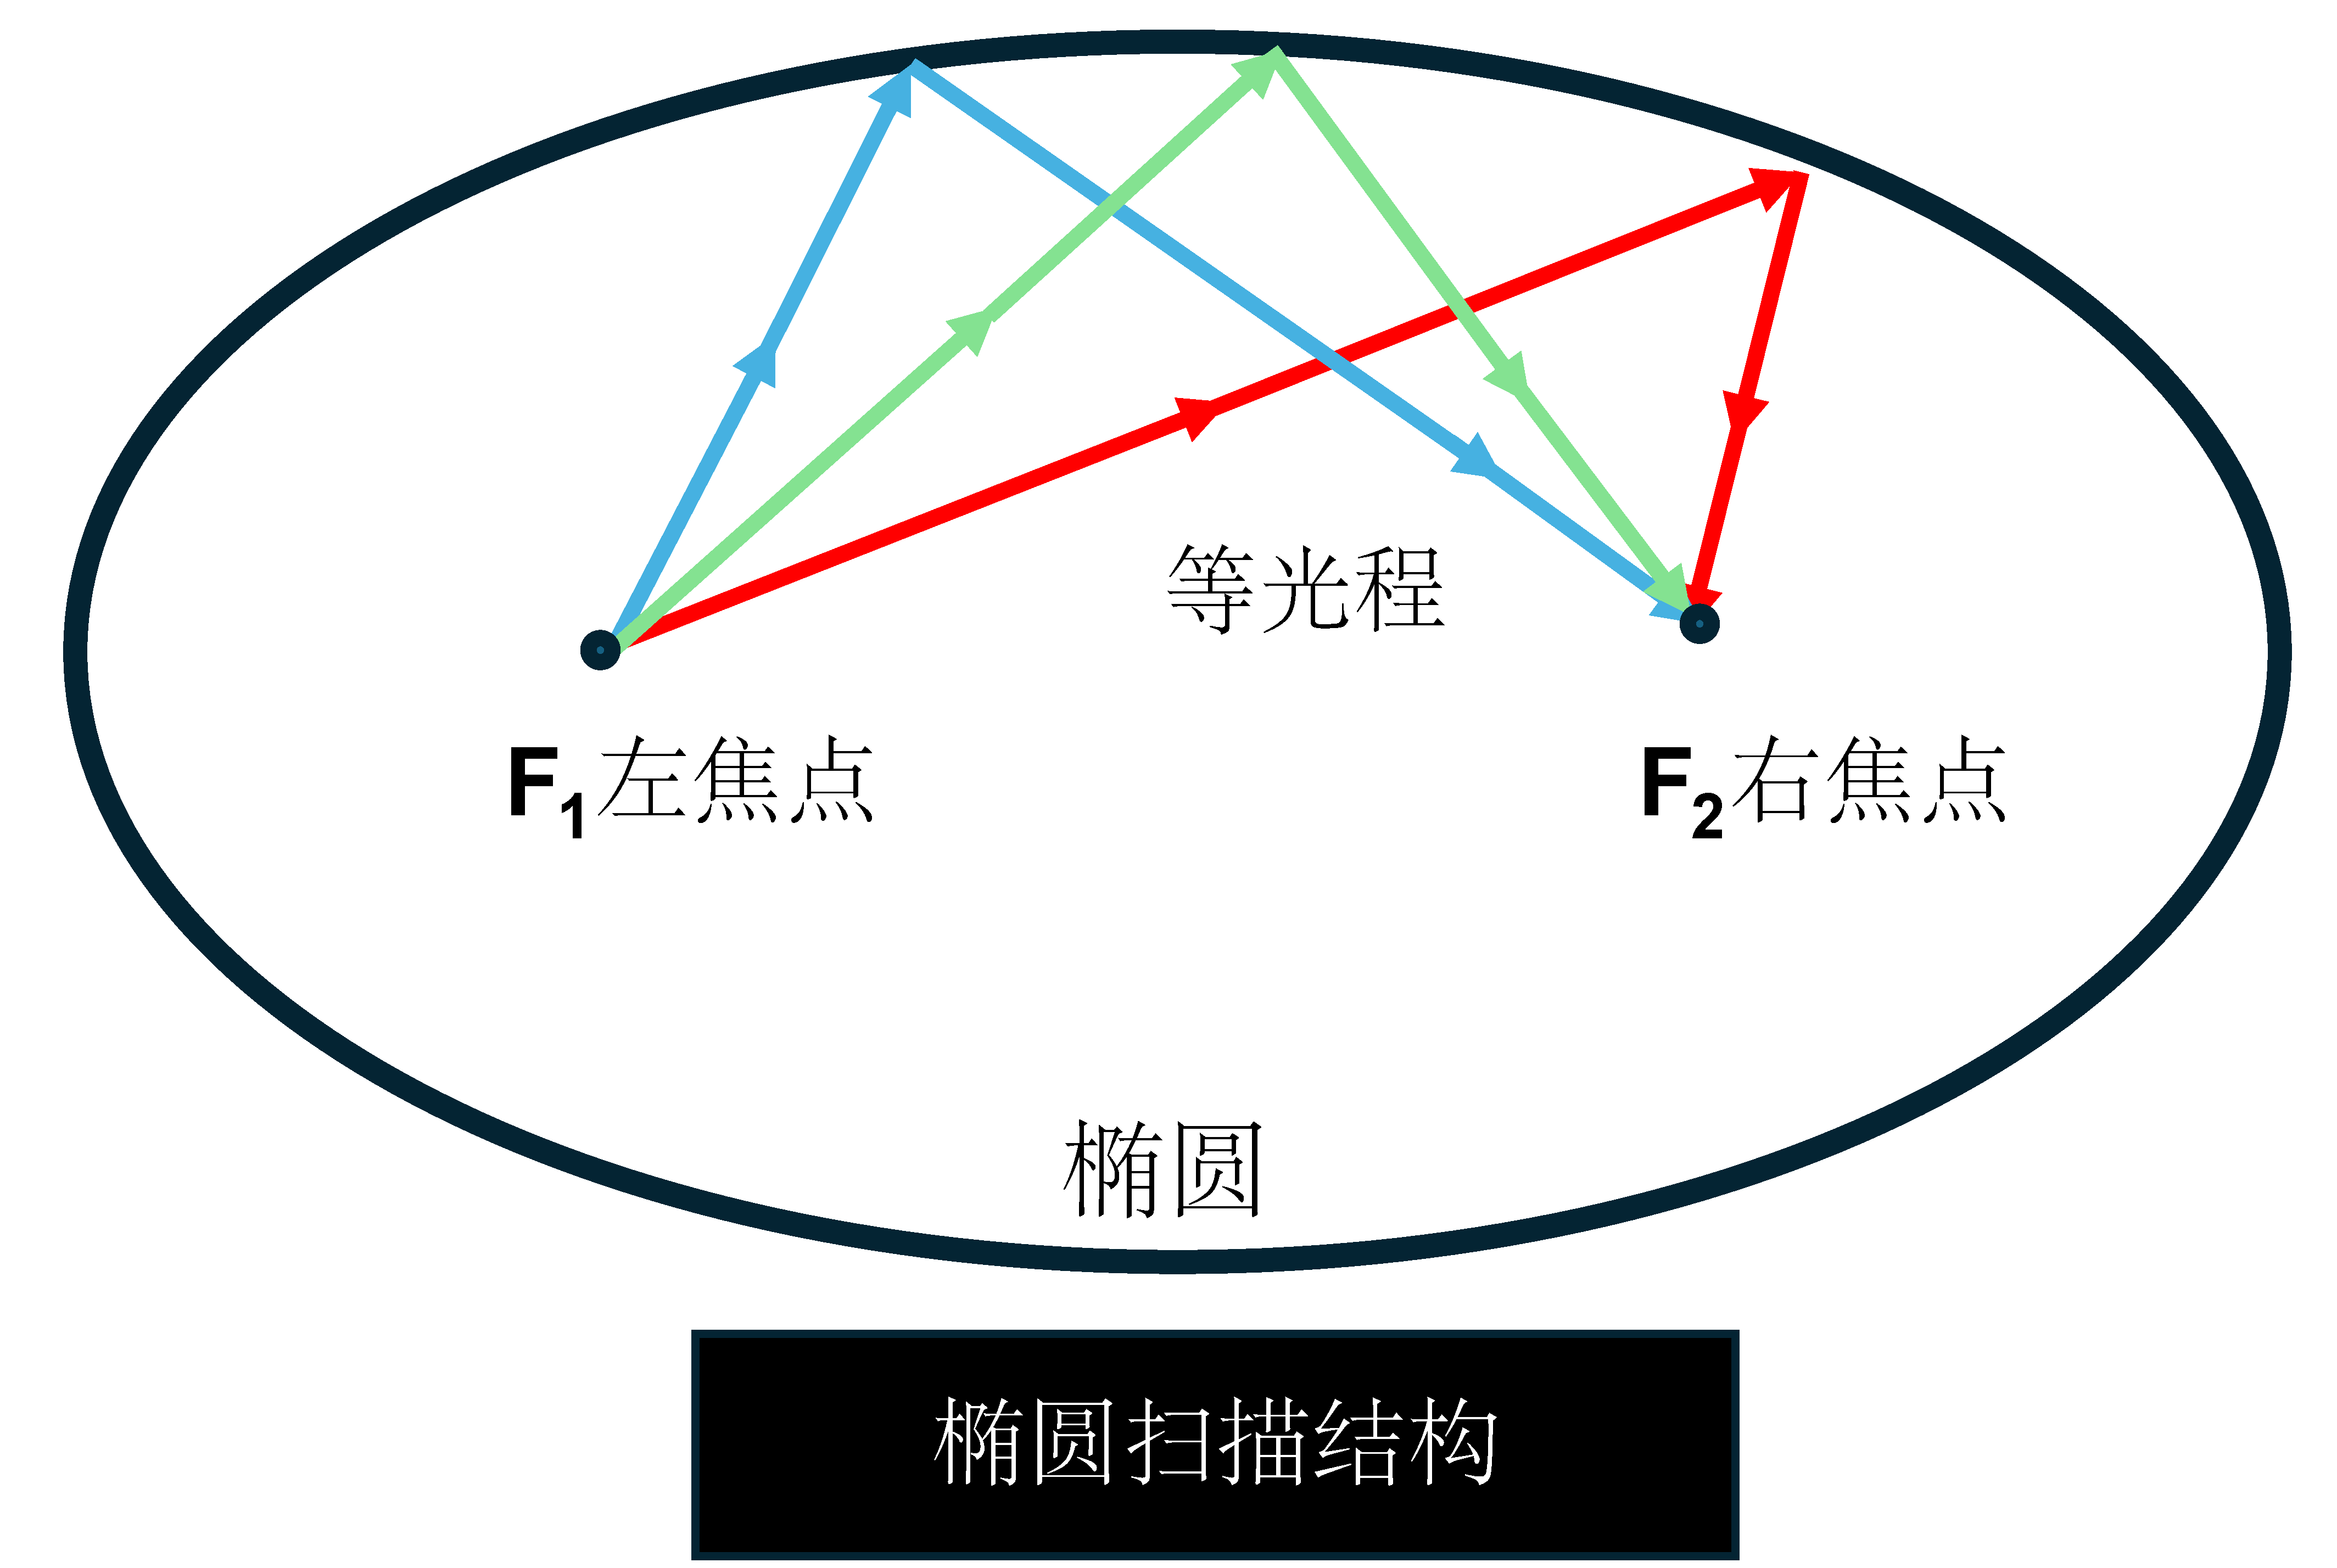
\includegraphics[width=\textwidth]{Fig/Fig59-1.pdf}
        \caption{}
        \label{fig59a}
    \end{subfigure}
    \hfil
    \begin{subfigure}[b]{0.47\textwidth}
        \centering
        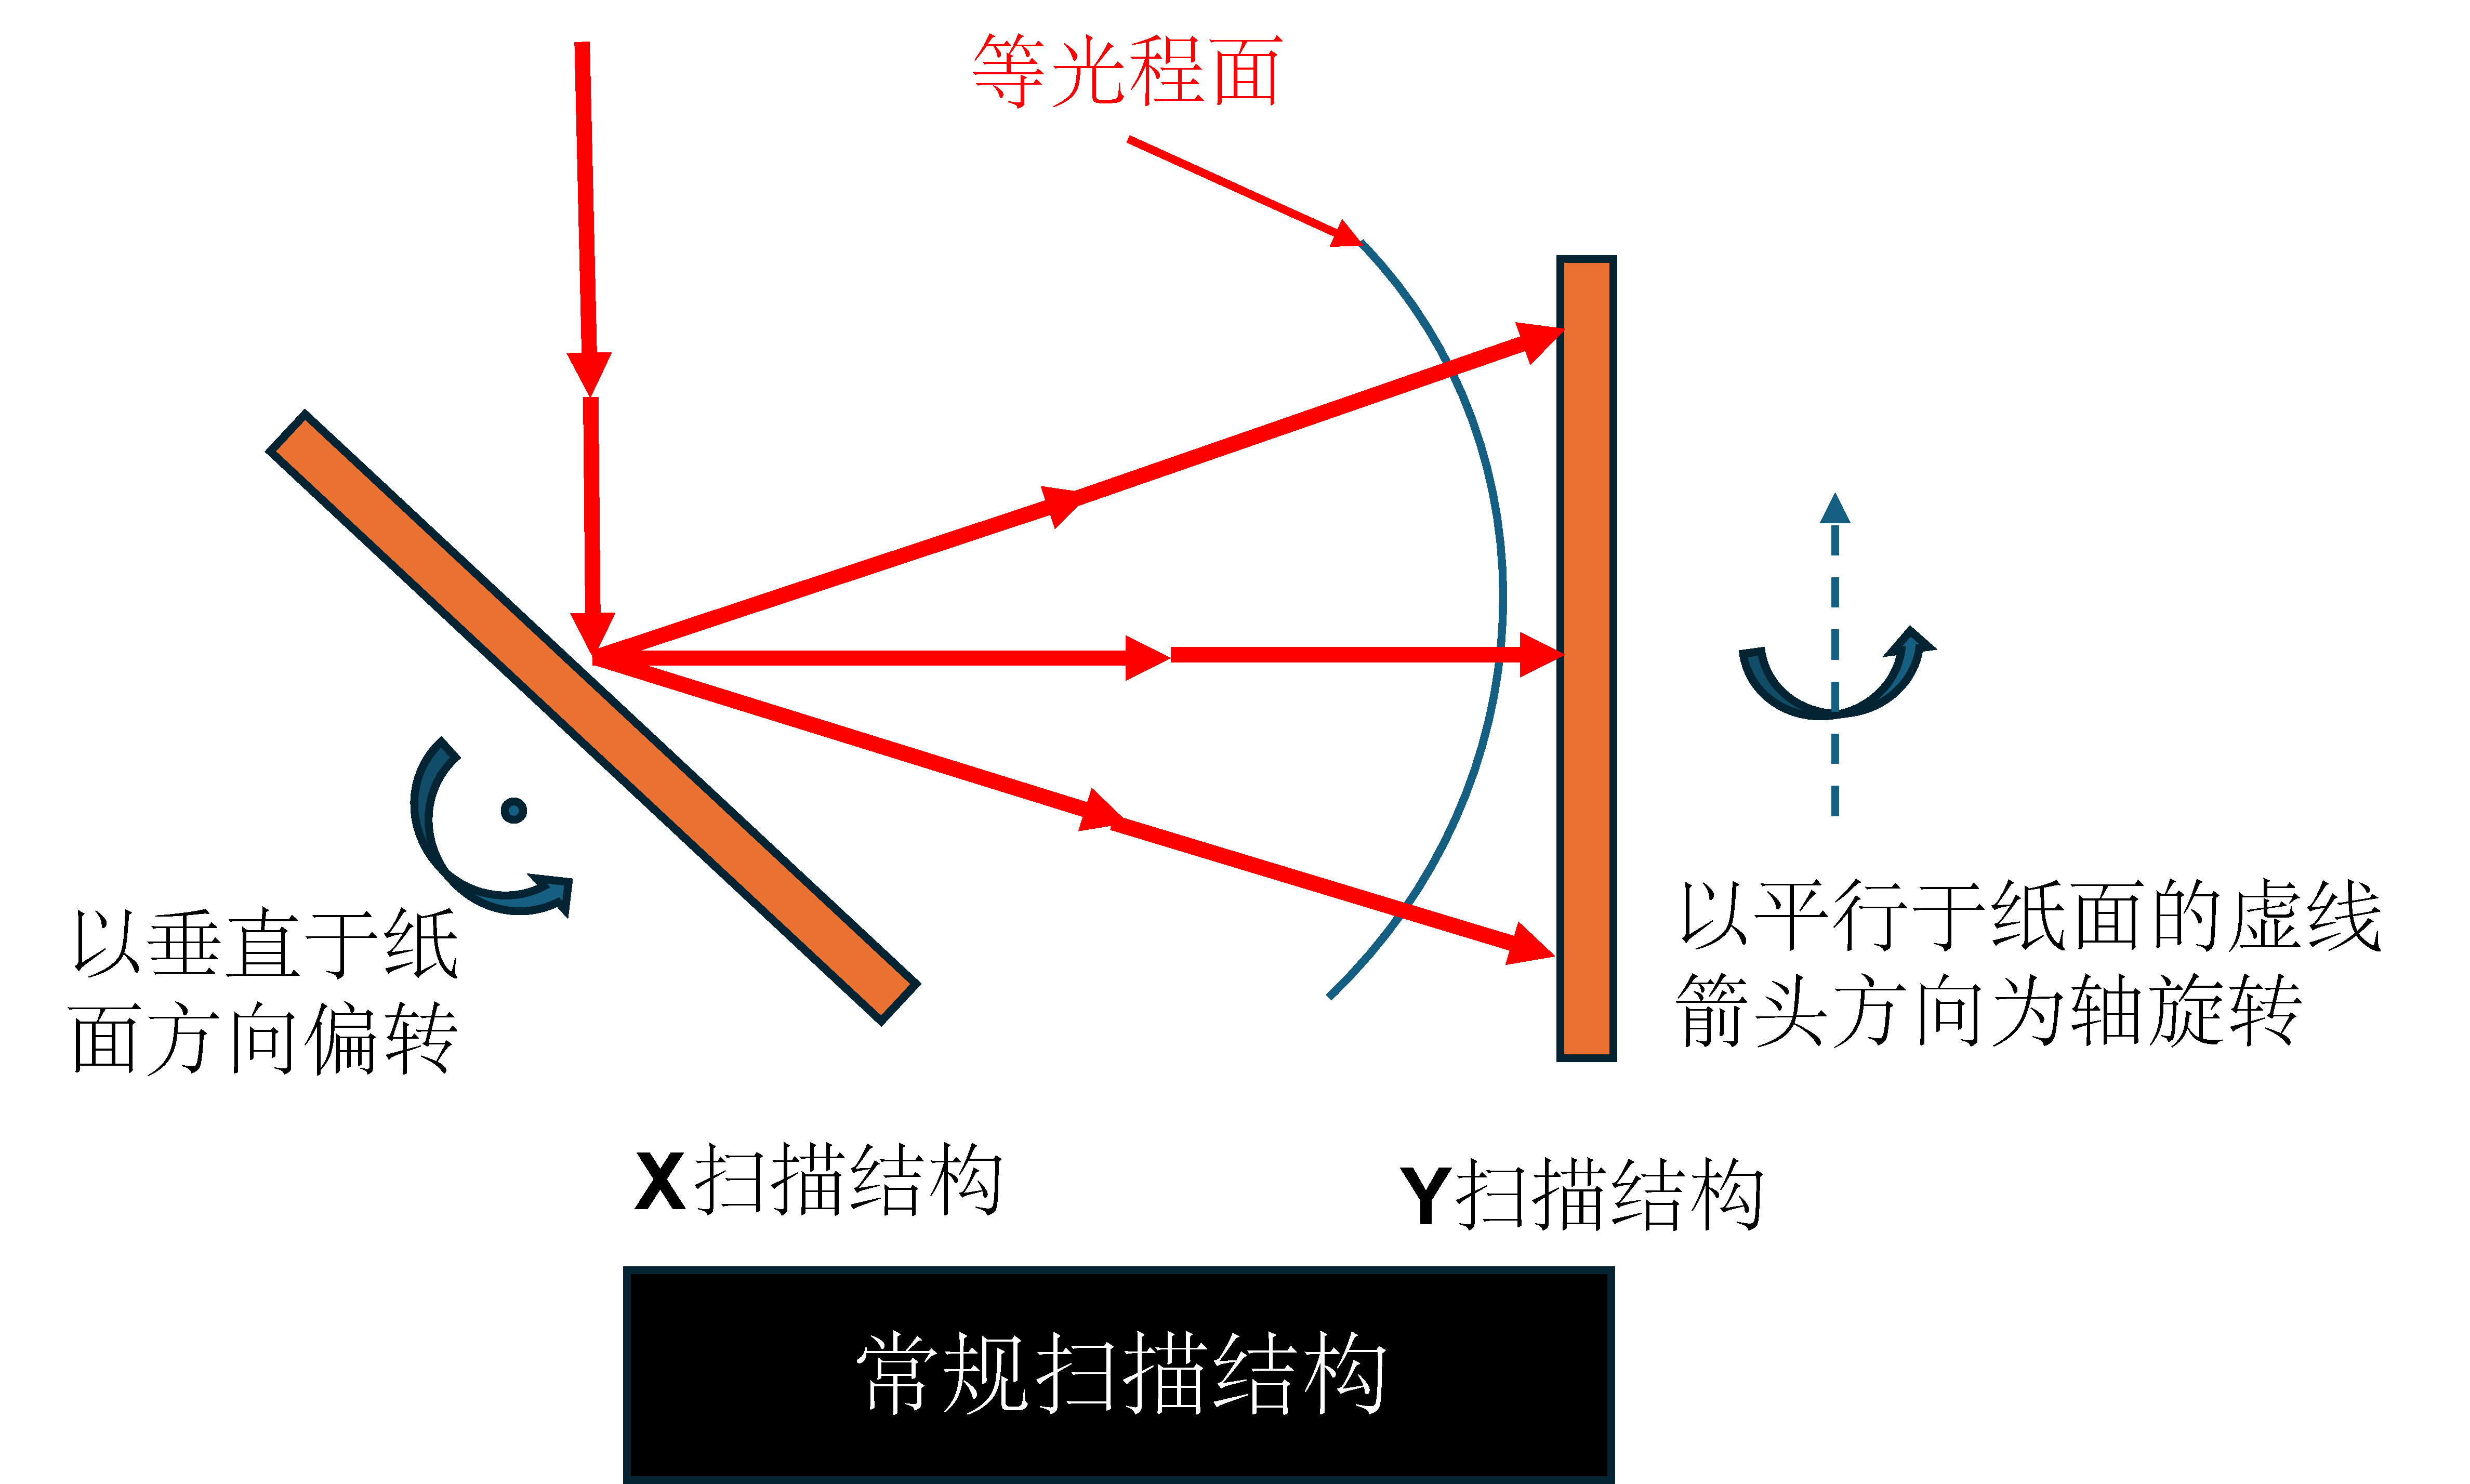
\includegraphics[width=\textwidth]{Fig/Fig59-2.pdf}
        \caption{}
        \label{fig59b}
    \end{subfigure}
    \bicaption{椭圆等光程扫描结构与常规扫描结构原理对比。(a) 基于椭圆反射面的等光程扫描结构；(b) 常规扫描结构}
    {Comparison between the elliptical equal-optical-path scanning structure and the conventional scanning structure. (a) Equal-optical-path scanning based on an elliptical reflective surface; (b) conventional scanning structure}
    \label{fig59}
\end{figure}

如图~\ref{fig59}(\subref{fig59a}) 所示，设椭圆的两个焦点分别为 $F_1$ 与 $F_2$。当扫描器件置于其中一个焦点附近时，扫描光束以不同角度入射到椭圆反射面后，均可在另一焦点处形成对应的聚焦或等效扫描输出。由于各条反射光线满足相同的几何光程，这种结构天然具备抑制扫描光程差的优势。

作为对比，图~\ref{fig59}(\subref{fig59b}) 给出了常规扫描结构示意。在传统平面或简单曲面反射扫描结构中，不同扫描角度下的传播路径通常并不完全一致，因此在大视场条件下更容易累积光程差，并进一步引入边缘视场畸变或扫描映射不均匀等问题。相比之下，椭圆反射面不仅能够改善边缘视场的光程一致性，还有望在较大视场范围内维持更稳定的扫描映射关系。

因此，从系统设计角度来看，采用椭圆反射面代替传统扫描反射结构，可以在不显著增加系统复杂度的前提下，对视场畸变进行主动校正，并为后续实现大视场、低畸变、均匀扫描的光学系统奠定基础。



\section{单椭圆结构的扫描速率非均匀性与双椭圆结构设计}\label{app:ellipse_3}

基于上述等光程原理，本文首先构建了单椭圆扫描结构。图~\ref{fig61}(\subref{fig61a}) 给出了单椭圆扫描结构的几何光路示意，图~\ref{fig61}(\subref{fig61b}) 则展示了其入射光与出射光扫描速率之间的关系。研究结果表明，单椭圆结构虽然能够有效改善传统扫描系统中的光程不等问题，但其输出扫描角与输入扫描角之间并不满足严格的线性关系。换言之，当振镜以恒定角速度扫描时，经椭圆面反射后的出射光并不会保持恒定的扫描角速度，而是会随入射角变化呈现出明显的非均匀性。

这种扫描速率的非均匀性将直接导致视场内不同位置的驻留时间发生变化。对于扫描成像系统而言，驻留时间的不一致不仅会引起局部采样密度变化，还可能导致图像亮度分布不均、边缘区域分辨率下降，甚至影响后续定量分析的准确性。因此，单椭圆结构虽然在光程均衡方面具有优势，但若要进一步应用于高精度、大视场成像系统，仍需对其扫描速率畸变进行额外补偿。

\begin{figure}[htbp]
    \centering
    \begin{subfigure}[b]{0.45\textwidth}
        \centering
        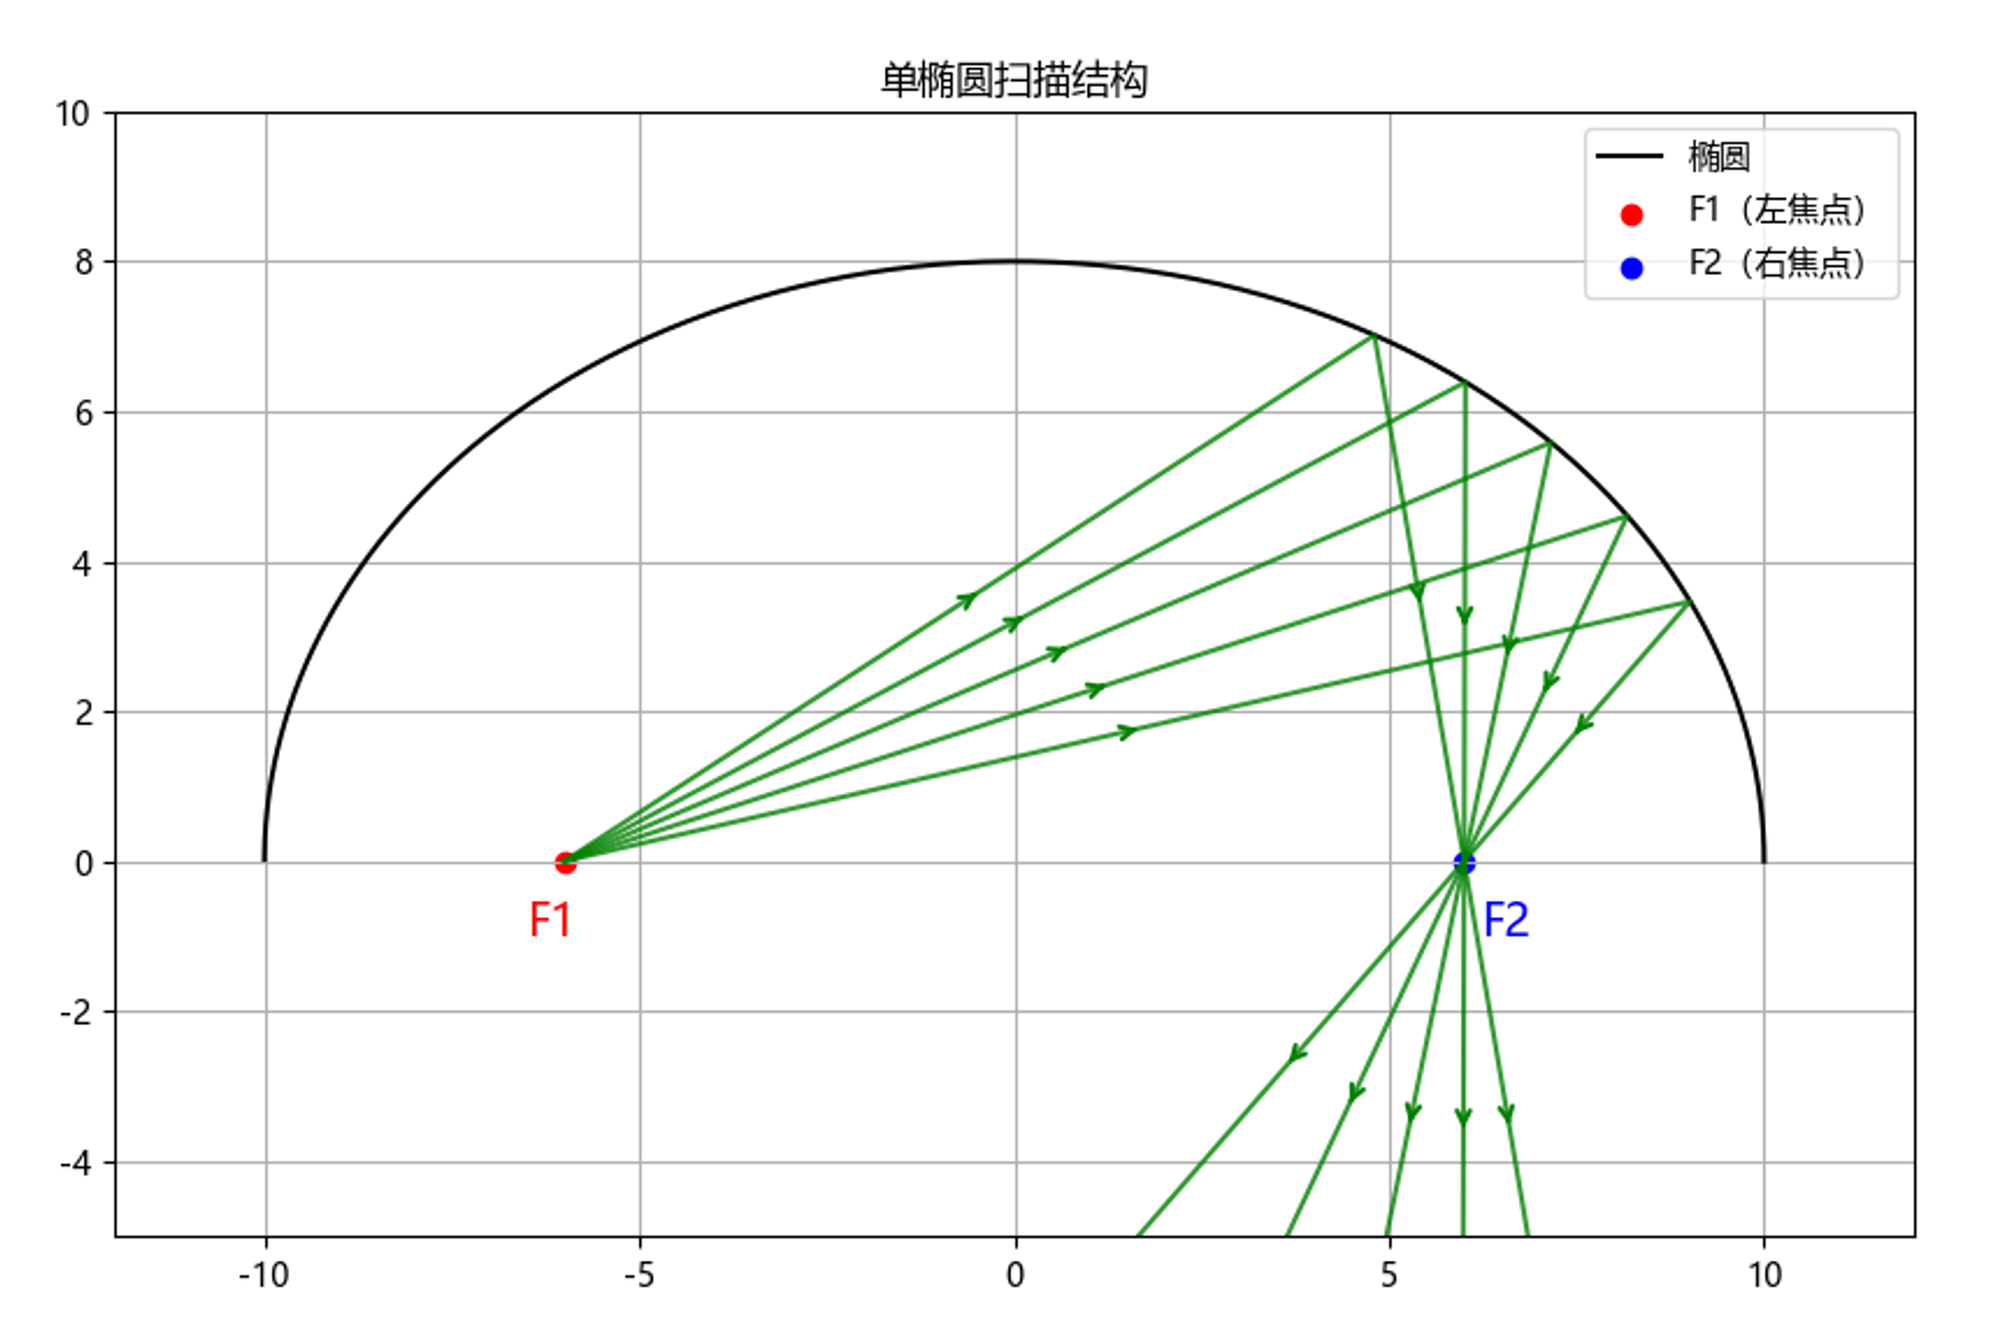
\includegraphics[width=\textwidth]{Fig/Fig61-1.png}
        \caption{}
        \label{fig61a}
    \end{subfigure}
    \hfil
    \begin{subfigure}[b]{0.47\textwidth}
        \centering
        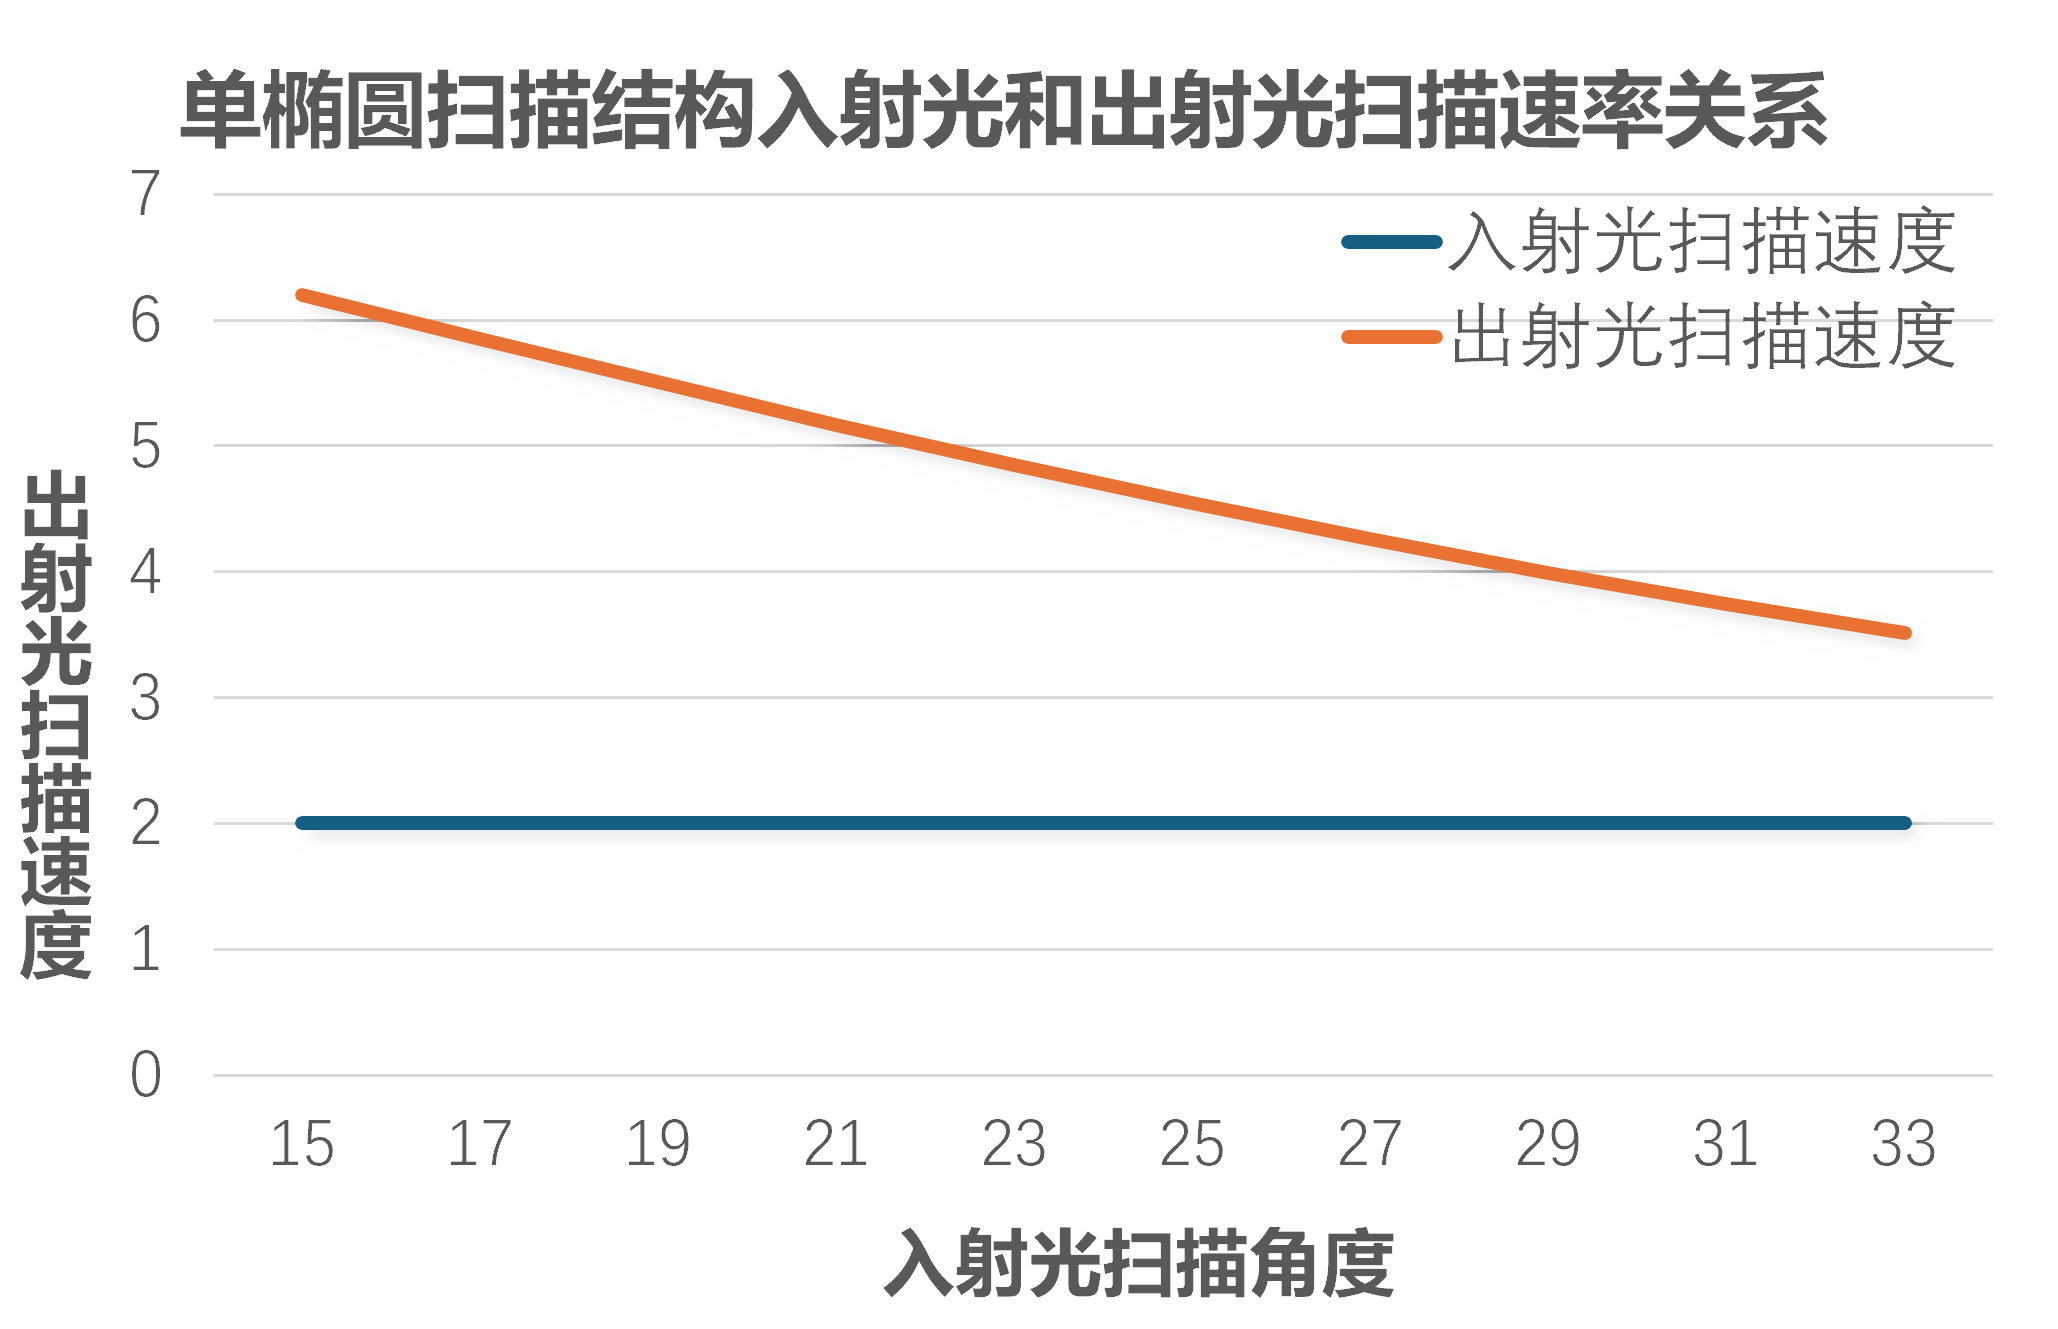
\includegraphics[width=\textwidth]{Fig/Fig61-2.png}
        \caption{}
        \label{fig61b}
    \end{subfigure}
    \bicaption{单椭圆扫描结构及其入射/出射光扫描速率关系。(a) 单椭圆等光程扫描结构示意；(b) 入射光与出射光扫描速率之间的非均匀关系}
    {Single-ellipse scanning structure and the relationship between input and output scan velocities. (a) Schematic of the single-ellipse equal-optical-path scanning structure; (b) nonuniform relationship between the input and output scan velocities}
    \label{fig61}
\end{figure}

针对这一问题，本文进一步提出了一种双椭圆级联扫描结构。该方案并非简单地将两个椭圆反射面串联，而是利用第一级椭圆实现等光程传递，再借助第二级椭圆对第一级引入的扫描速率非线性进行补偿，从而同时兼顾``光程均衡''和``扫描匀速''两方面需求。双椭圆结构的系统功能框图如图~\ref{fig:fig49_52_62}(\subref{fig:fig49}) 所示，其核心思想是通过引入中间虚拟像面，使两个椭圆模块在几何映射上形成协同配合：第一级完成视场展开与初步映射，第二级则对扫描速率进行反向校正，最终获得更均匀的出射扫描特性。其相应的光线追迹与几何关系如图~\ref{fig:fig49_52_62}(\subref{fig:fig62a}) 所示，而双椭圆结构对扫描速率非线性的补偿效果则如图~\ref{fig:fig49_52_62}(\subref{fig:fig62b}) 所示。

从设计思路上看，这种双级联结构的优势在于：单一椭圆面只能解决一个主要矛盾，即光程均衡或角度映射优化中的某一部分，而双椭圆结构则通过自由度的增加，使系统能够在多个性能指标之间实现更优折中。也正因如此，双椭圆方案相比单椭圆方案更适用于需要兼顾大视场、低畸变与高扫描均匀性的应用场景。

在完成双椭圆级联系统的总体构型设计之后，下一步关键问题在于确定两个椭圆反射面的参数匹配关系。由于第二级椭圆承担着对第一级扫描速率畸变进行补偿的功能，其离心率选取将直接影响最终系统的匀速扫描效果。因此，有必要对双椭圆结构的几何参数进行系统性优化，以获得最佳的速率补偿性能。

\begin{figure}[htbp]
    \centering

    \begin{subfigure}[b]{0.48\textwidth}
        \centering
        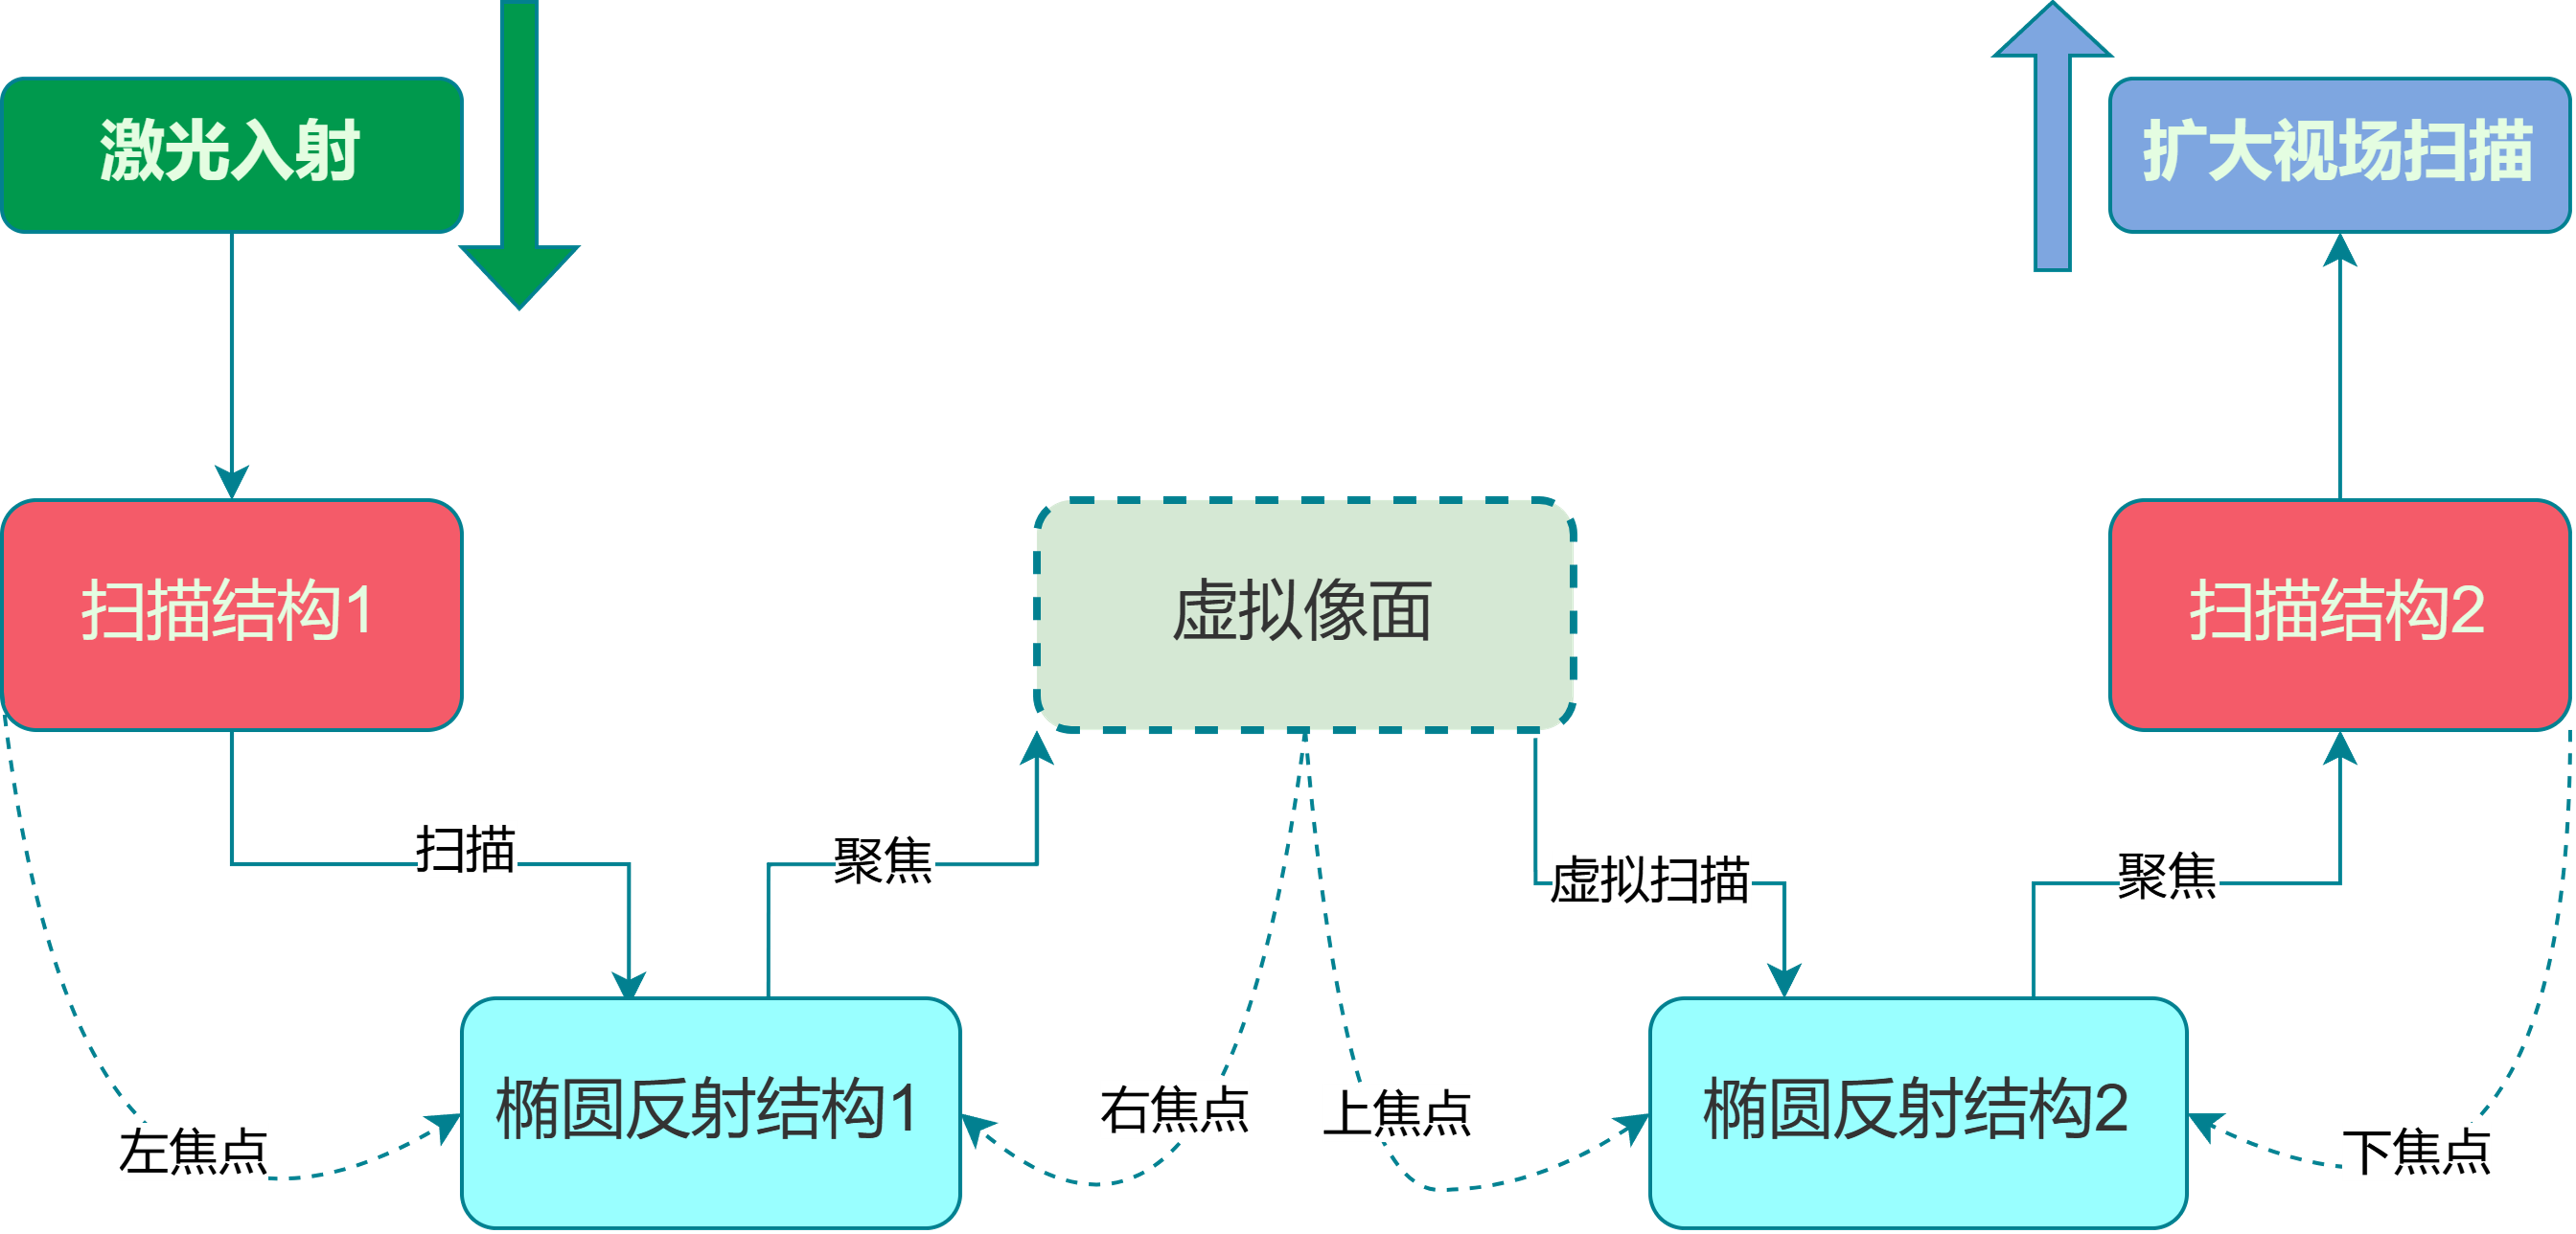
\includegraphics[width=0.9\textwidth]{Fig/Fig49.png}
        \caption{}
        \label{fig:fig49}
    \end{subfigure}
    \hfil
    \begin{subfigure}[b]{0.48\textwidth}
        \centering
        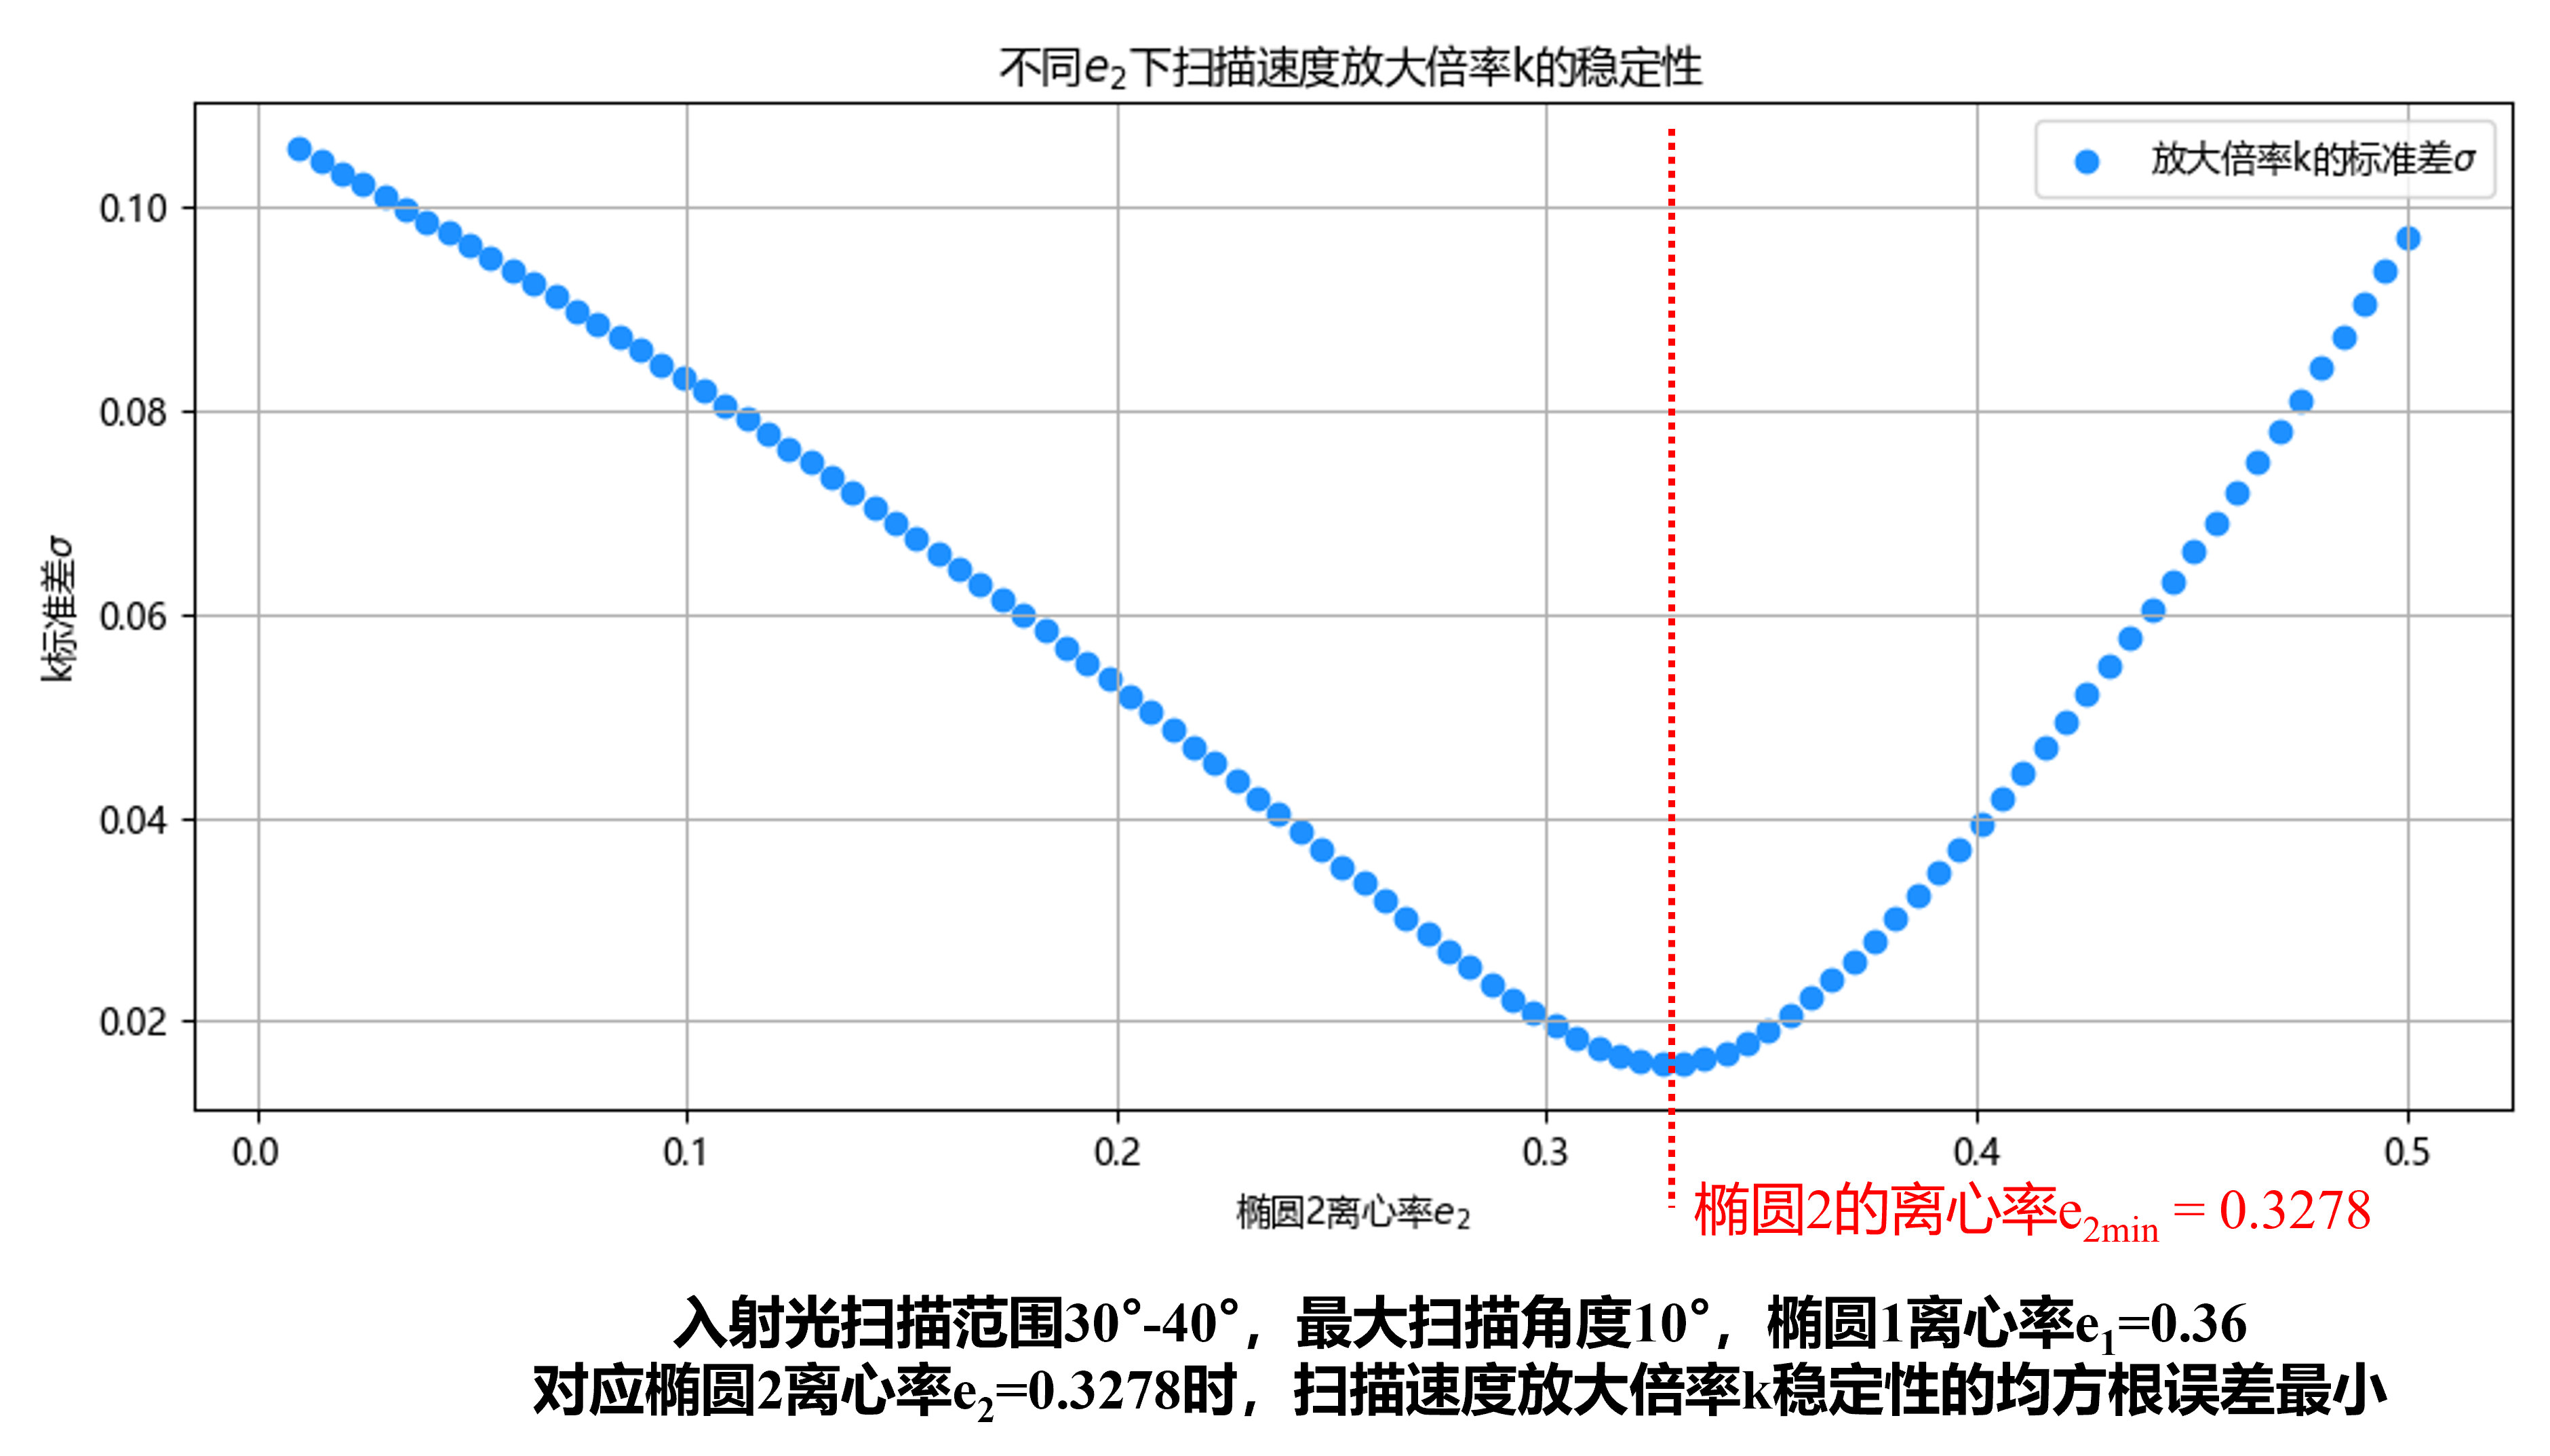
\includegraphics[width=0.9\textwidth]{Fig/Fig52.png}
        \caption{}
        \label{fig:fig52}
    \end{subfigure}

    \vspace{1em}

    \begin{subfigure}[b]{0.33\textwidth}
        \centering
        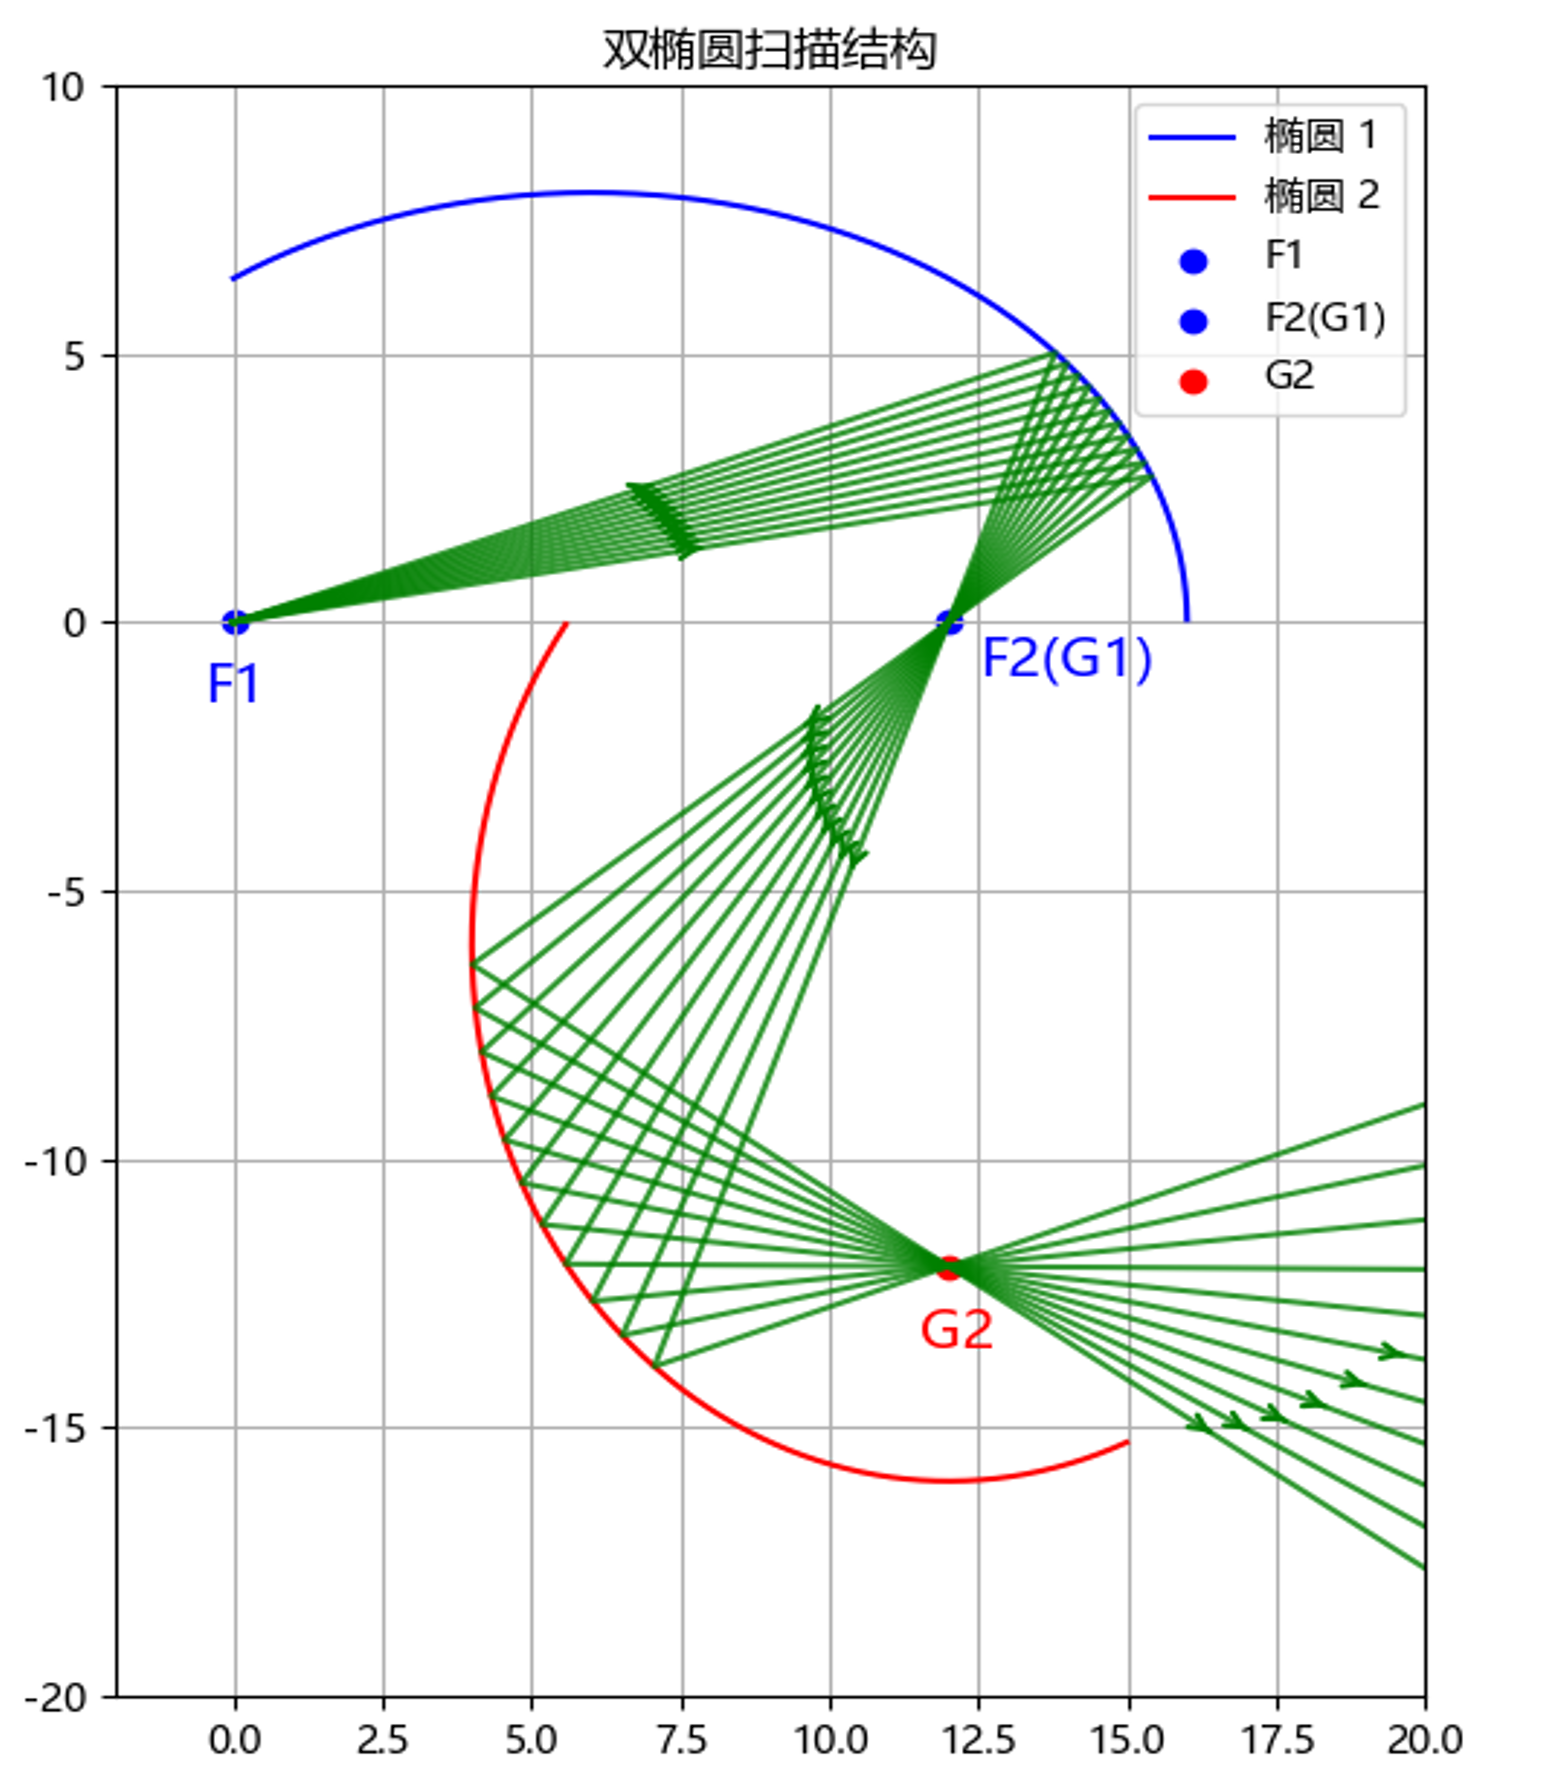
\includegraphics[width=0.9\textwidth]{Fig/Fig62-1.png}
        \caption{}
        \label{fig:fig62a}
    \end{subfigure}
    \hfil
    \begin{subfigure}[b]{0.58\textwidth}
        \centering
        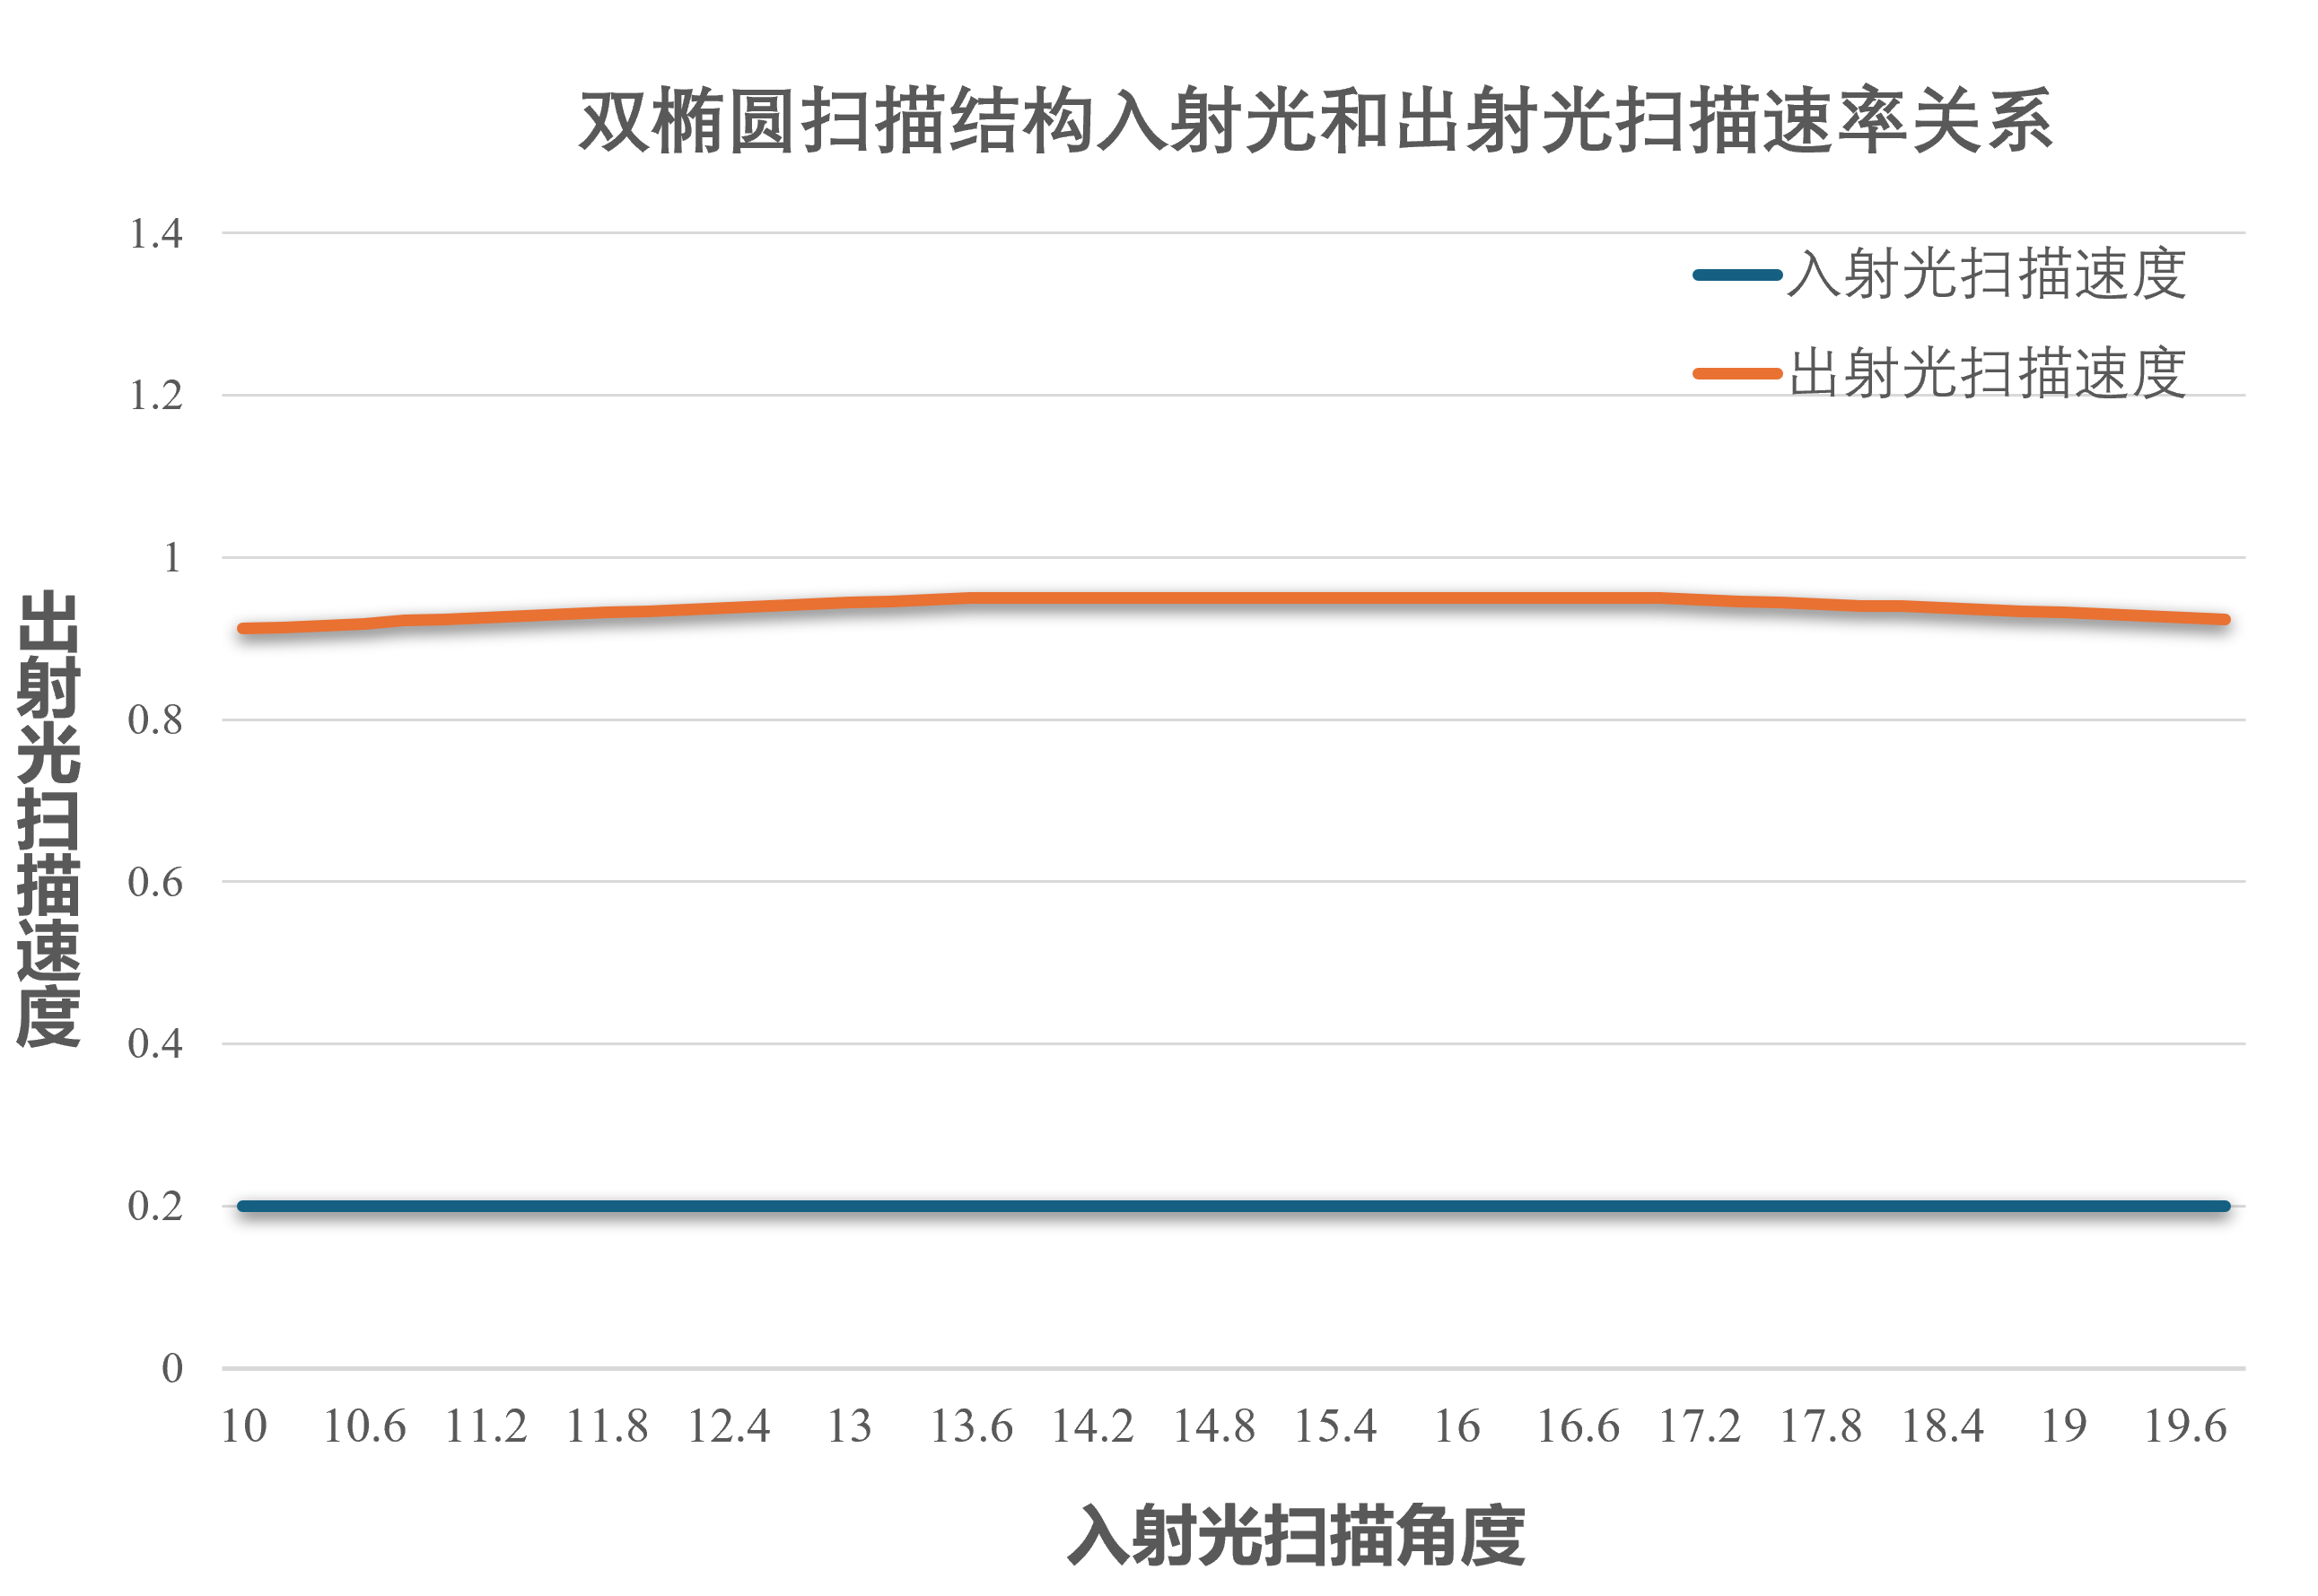
\includegraphics[width=0.9\textwidth]{Fig/Fig62-2.png}
        \caption{}
        \label{fig:fig62b}
    \end{subfigure}

    \bicaption{双椭圆扫描系统功能框图、参数优化及扫描特性分析。(a) 双椭圆级联匀速扫描系统功能框图；(b) 不同 $e_2$ 下扫描速度放大倍率 $k$ 的稳定性分析；(c) 双椭圆扫描结构的光线追迹与几何关系；(d) 双椭圆扫描结构中入射光与出射光的扫描速率关系}
    {Functional block diagram, parameter optimization, and scanning-characteristic analysis of the double-ellipse scanning system. (a) Functional block diagram of the cascaded uniform-speed double-ellipse scanner; (b) stability analysis of the scan-velocity magnification factor $k$ under different $e_2$ values; (c) ray-tracing and geometric relationship of the double-ellipse scanning structure; (d) relationship between the input and output scan velocities in the double-ellipse scanning structure}
    \label{fig:fig49_52_62}
\end{figure}

为实现最佳的补偿效果，本文对两个椭圆的离心率参数进行了系统寻优。如图~\ref{fig:fig49_52_62}(\subref{fig:fig52}) 所示，在保持第一级椭圆离心率恒定的条件下，通过比较不同第二级椭圆离心率 $e_2$ 对扫描放大倍率 $k$ 稳定性的影响，可以观察到系统输出均匀性随参数变化呈现明显差异。当第二级椭圆离心率取 $e_{2\min}=0.3278$ 时，放大倍率波动的标准差 $\sigma$ 达到最小值，说明此时系统的扫描速率最接近理想匀速状态。该结果表明，通过合理匹配两个椭圆的几何参数，第二级椭圆能够在较大程度上抵消第一级椭圆所带来的非线性扫描效应。

经过参数优化与结构校正后，双椭圆系统在全视场范围内表现出较高的扫描均匀性。最终结果如图~\ref{fig:fig49_52_62}(\subref{fig:fig62b}) 所示，在目标扫描范围内，出射角对时间的变化关系近似线性，其最大偏差仅为 $3.65\%$，均方根误差(RMSE)低至 $0.19$。这表明所提出的双椭圆级联系统已能够较好地逼近理想匀速扫描模型。相比传统扫描结构，该方法不仅改善了几何光程分布，还显著提升了扫描动态特性的一致性。

此外，该双椭圆架构在实现匀速扫描的同时，还具备明显的扫描视场放大能力。如图~\ref{fig:fig49_52_62}(\subref{fig:fig62a}) 所示，输入端振镜仅需提供约 $0.5^\circ$ 的微小扫描角，经双椭圆结构放大后，输出端即可获得约 $5^\circ$ 的有效扫描视场。这意味着该结构可在不显著增加前端扫描器件负担的前提下，实现更大的输出视场范围，从而提升系统在大范围成像、高速扫描以及紧凑型仪器设计中的应用潜力。换言之，双椭圆结构不仅是一种几何补偿方案，同时也是一种兼具视场扩展能力的扫描放大架构。

\begin{figure}[htbp]
    \centering

    \begin{subfigure}[t]{0.32\textwidth}
        \centering
        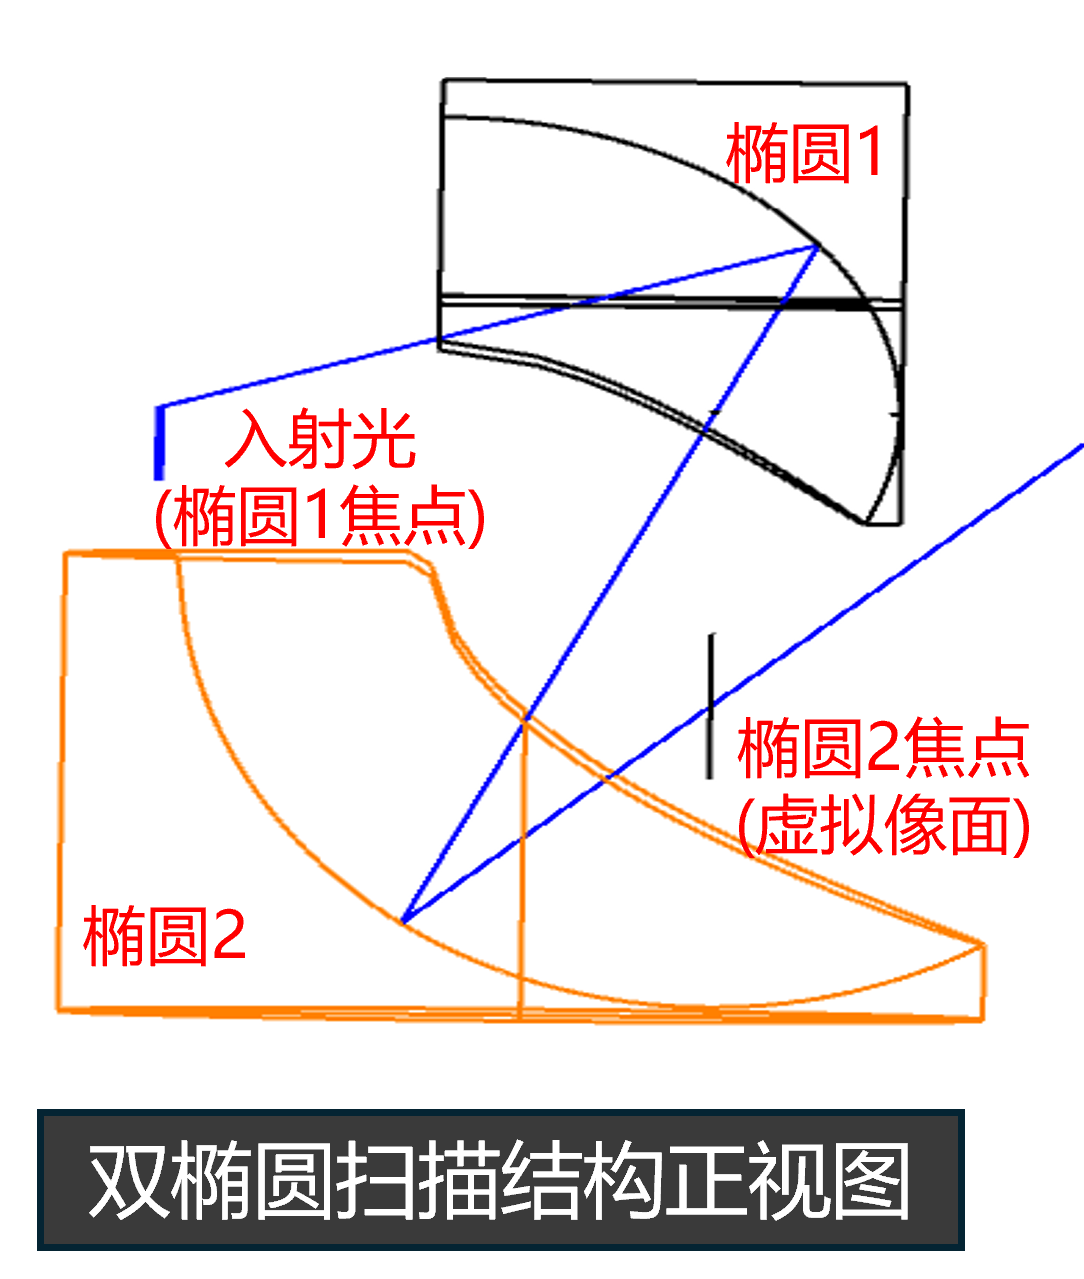
\includegraphics[width=\linewidth]{Fig/Fig53-1.png}
        \caption{}
        \label{fig53a}
    \end{subfigure}
    \hfil
    \begin{subfigure}[t]{0.32\textwidth}
        \centering
        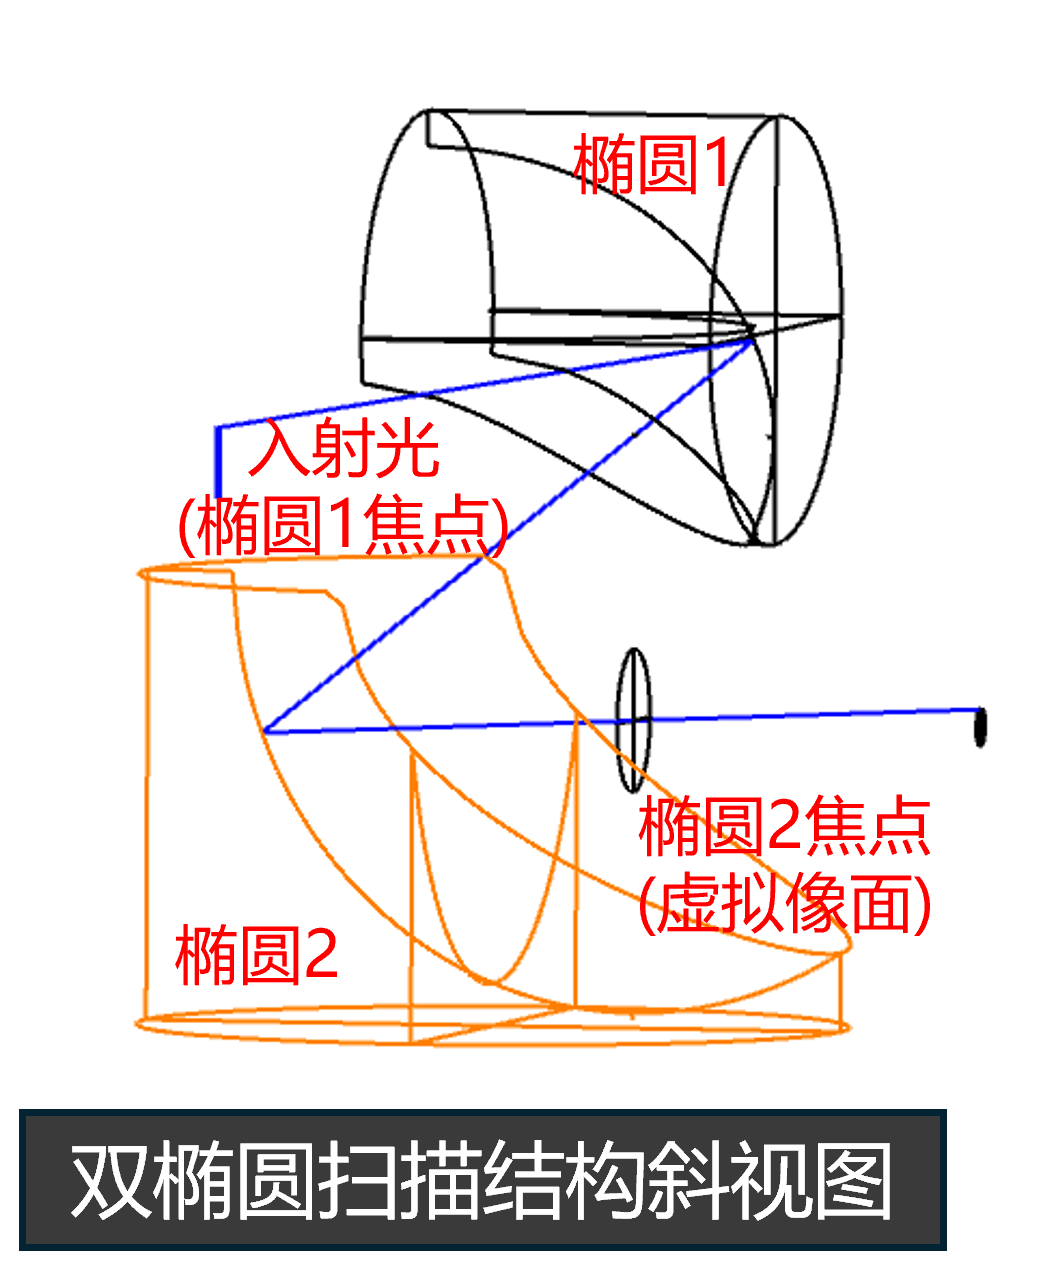
\includegraphics[width=\linewidth]{Fig/Fig53-2.png}
        \caption{}
        \label{fig53b}
    \end{subfigure}
    \hfil
    \begin{subfigure}[t]{0.34\textwidth}
        \centering
        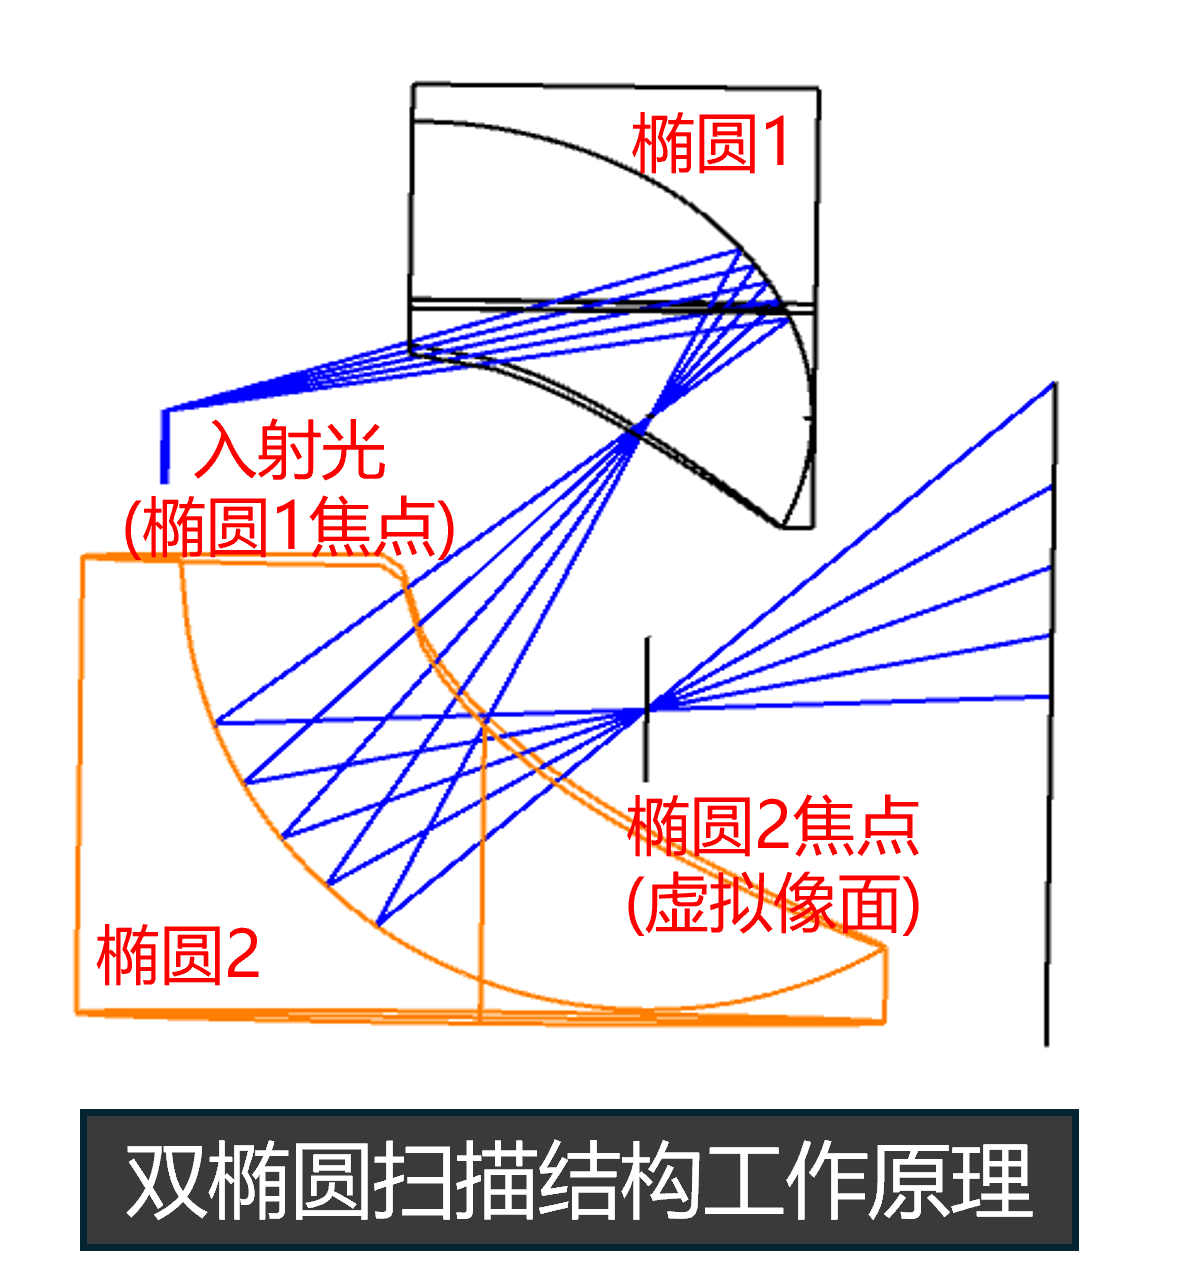
\includegraphics[width=\linewidth]{Fig/Fig53-3.png}
        \caption{}
        \label{fig53c}
    \end{subfigure}

    \bicaption{双椭圆扫描结构的三视图与工作原理示意图。(a) 正视图；(b) 斜视图；(c) 工作原理图}
    {Three views and operating principle of the double-ellipse scanning structure. (a) Front view; (b) perspective view; (c) working principle}
    \label{fig53}
\end{figure}

为了进一步验证双椭圆级联扫描结构在实际光学系统中的可实现性与成像性能，本文在 Ansys Zemax OpticStudio 中建立了该系统的三维实体模型，并开展了详细的光线追迹与像差分析。

图~\ref{fig53}(\subref{fig53a})--(\subref{fig53c}) 展示了双椭圆扫描结构在 Zemax 中的正视图、斜视图及三维工作原理图。如图所示，入射光首先汇聚于第一级椭圆面的焦点附近，经第一级椭圆反射后在两个椭圆共享的中间焦点处形成虚拟像面，随后再由第二级椭圆反射并输出。该三维模型不仅直观再现了双焦点共轭和等光程传递机制，也验证了双椭圆级联系统在空间布局上的可实现性。与二维几何推导相比，三维仿真进一步说明该结构并非仅在理想平面模型中有效，而是具备向实际工程系统转化的可能。


\begin{figure}[htbp]
    \centering
    \begin{subfigure}[t]{0.38\textwidth}
        \centering
        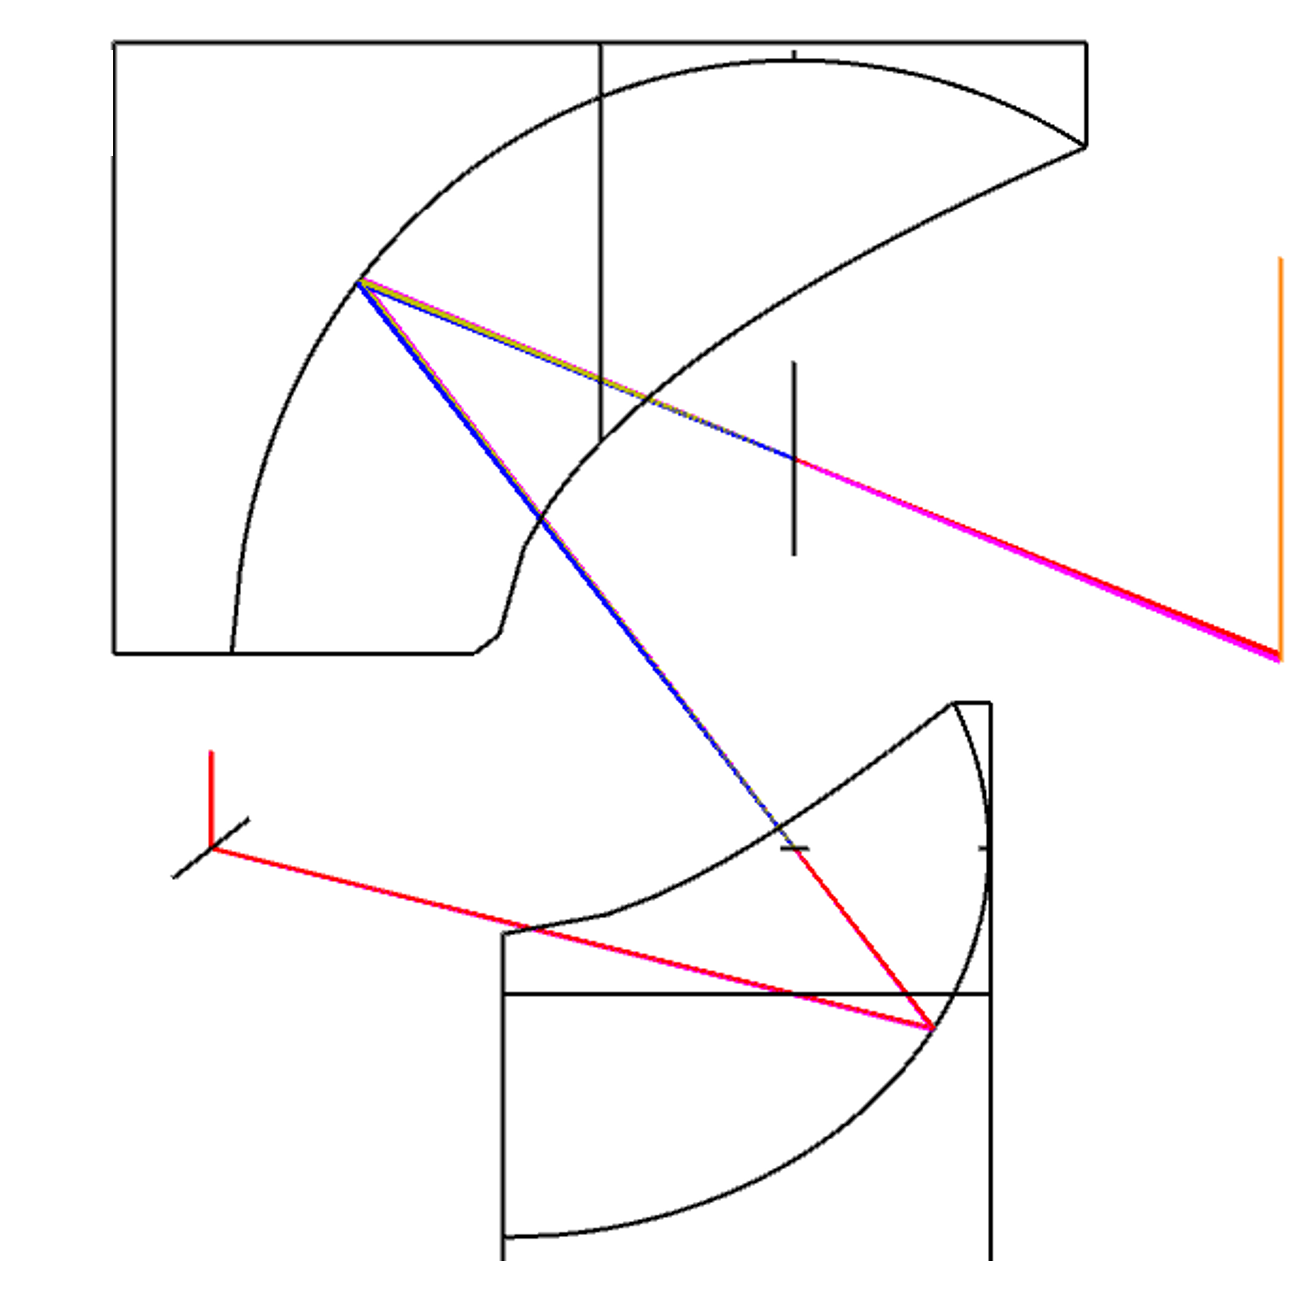
\includegraphics[width=\linewidth]{Fig/Fig56-1.png}
        \caption{光路布局图}
        \label{fig56a}
    \end{subfigure}
    \hfil
    \begin{subfigure}[t]{0.48\textwidth}
        \centering
        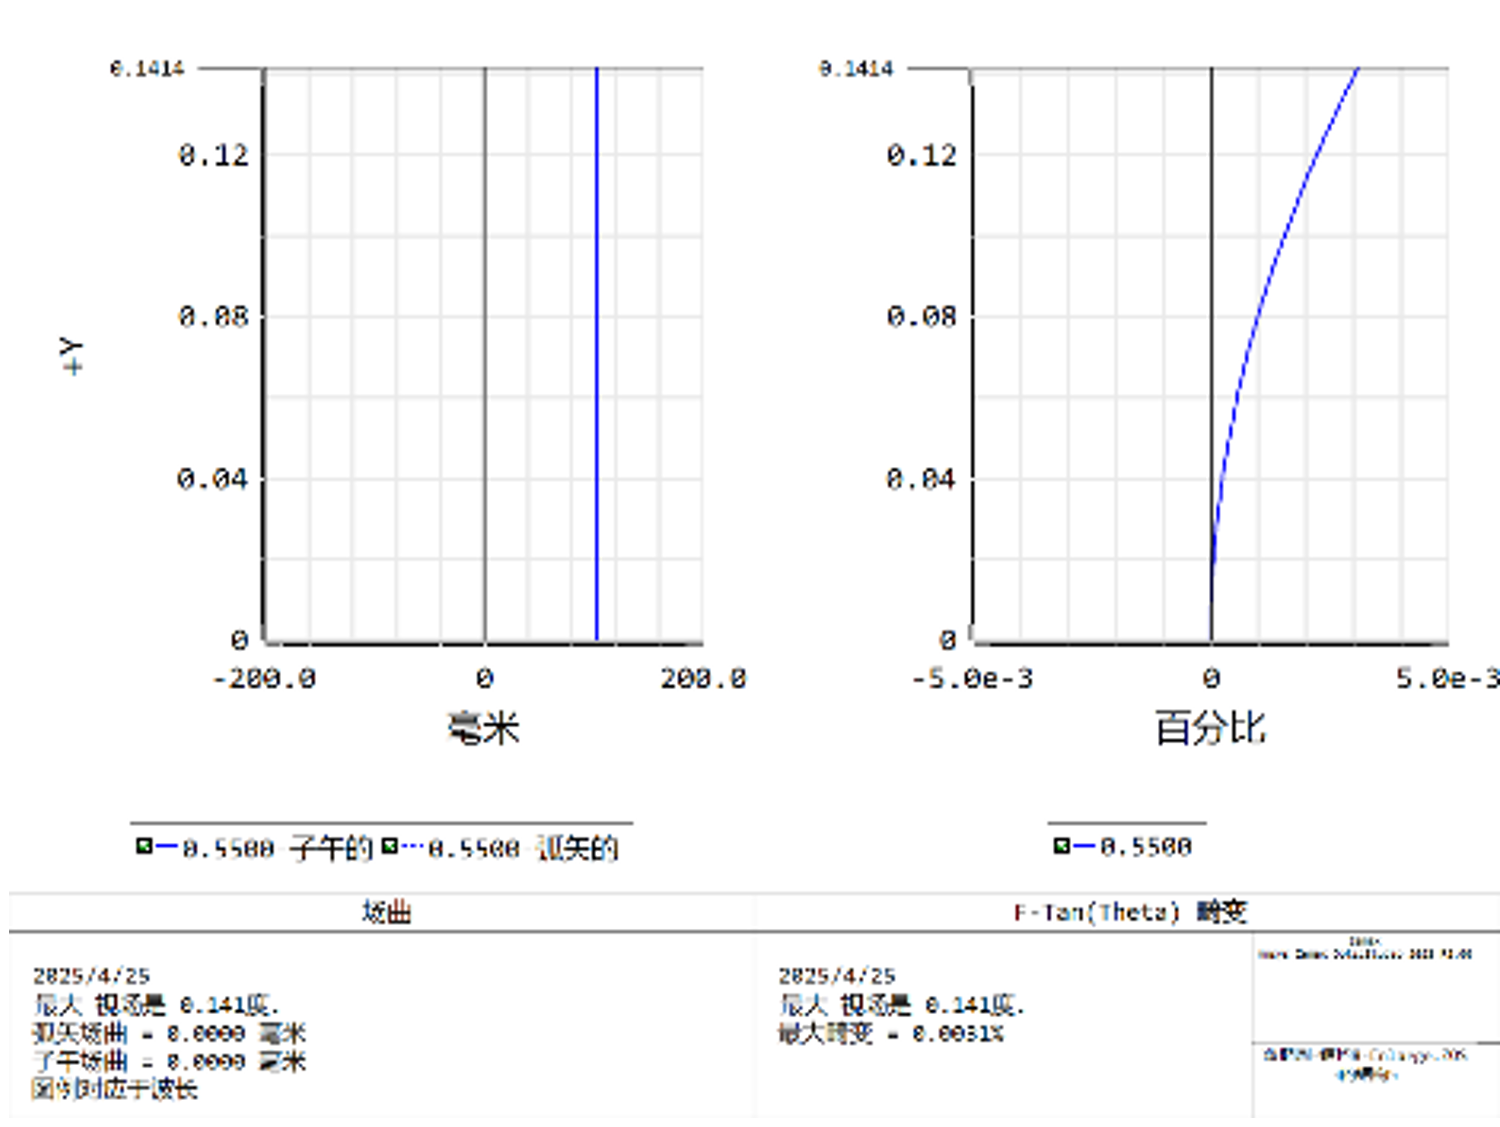
\includegraphics[width=\linewidth]{Fig/Fig56-2.png}
        \caption{像场弯曲与 $F$-$\tan(\theta)$ 畸变曲线}
        \label{fig56b}
    \end{subfigure}

    \vspace{0.4em}

    \begin{subfigure}[t]{0.48\textwidth}
        \centering
        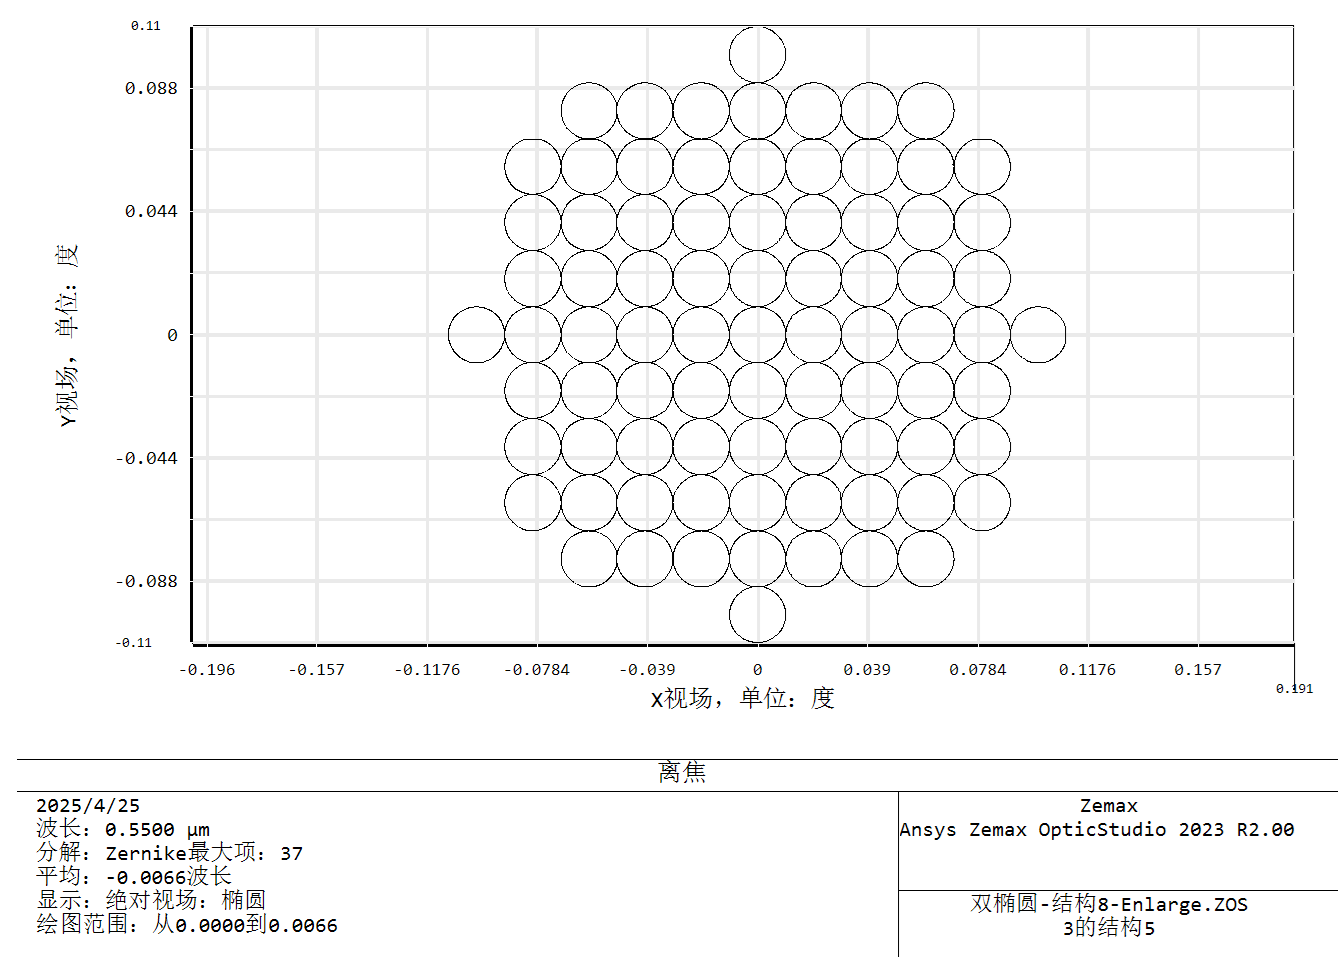
\includegraphics[width=\linewidth]{Fig/Fig56-3.png}
        \caption{全视场点列图}
        \label{fig56c}
    \end{subfigure}
    \hfil
    \begin{subfigure}[t]{0.46\textwidth}
        \centering
        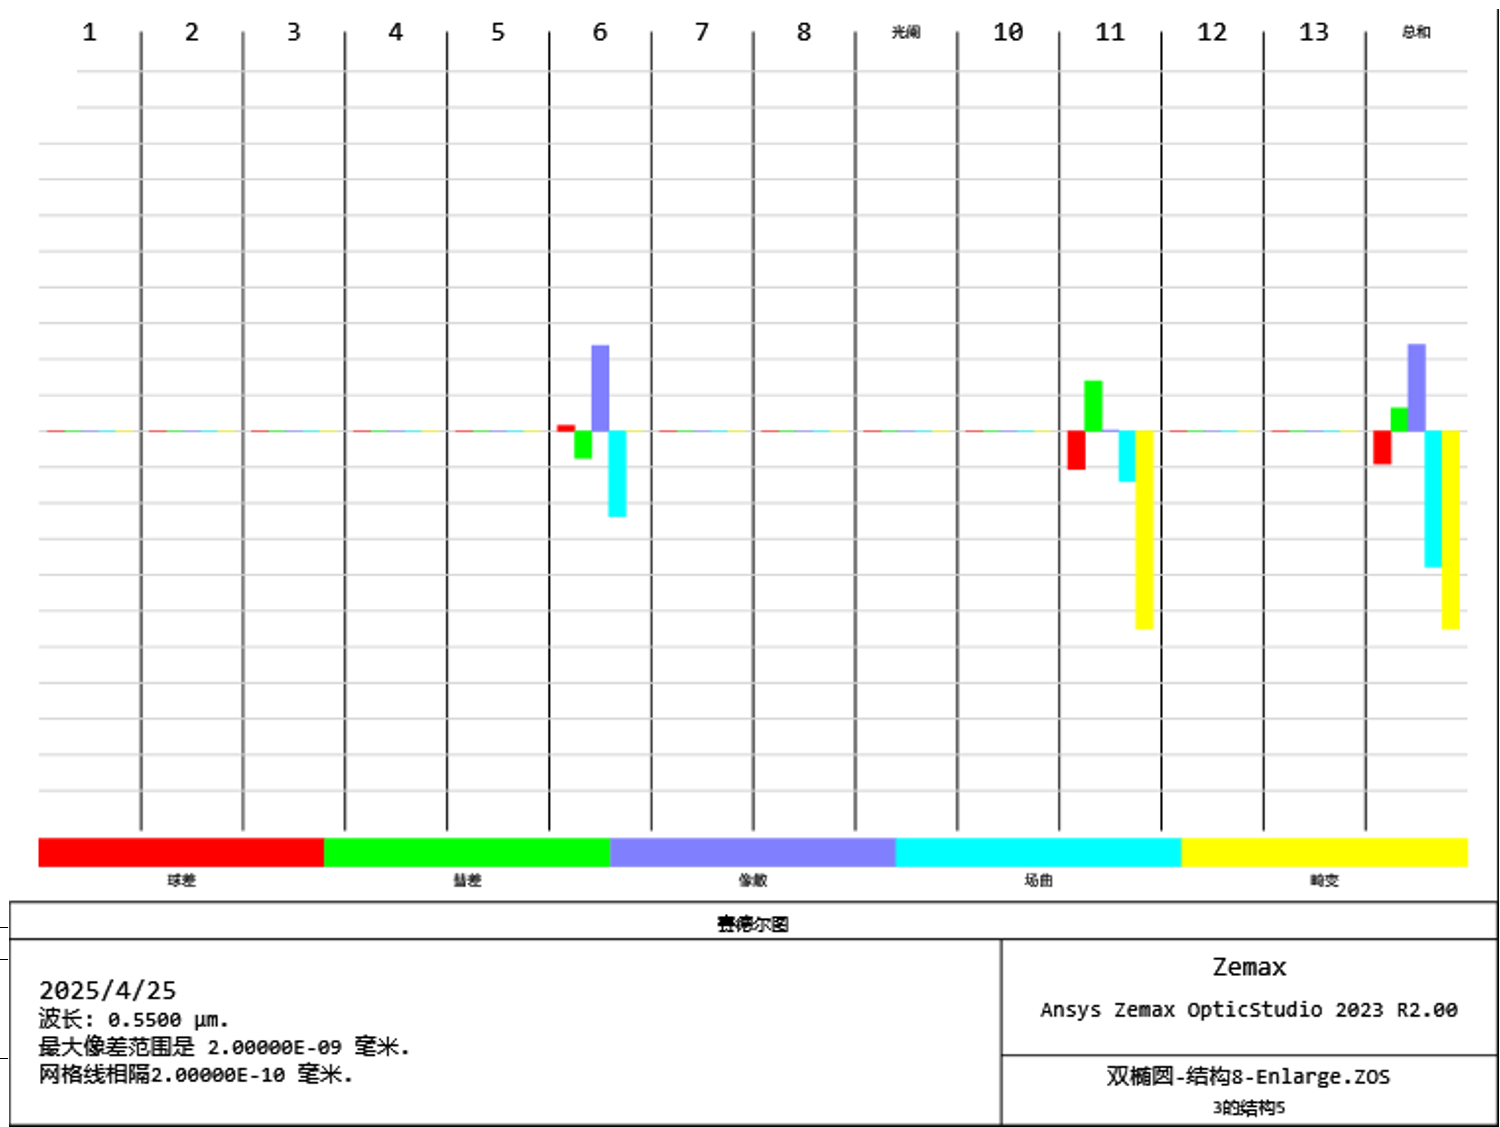
\includegraphics[width=\linewidth]{Fig/Fig56-4.png}
        \caption{塞德尔像差系数图}
        \label{fig56d}
    \end{subfigure}

    \bicaption{双椭圆扫描结构的像差与像质分析结果。(a) 光路布局图；(b) 像场弯曲与 $F$-$\tan(\theta)$ 畸变曲线；(c) 全视场点列图；(d) 塞德尔像差系数图}
    {Aberration and image-quality analysis of the double-ellipse scanning structure. (a) Optical layout; (b) field curvature and $F$-$\tan(\theta)$ distortion; (c) full-field spot diagram; (d) Seidel aberration coefficients}
    \label{fig56}
\end{figure}

为了进一步评估双椭圆结构的综合光学表现，本文对系统的关键像差参数进行了分析，结果如图~\ref{fig56} 所示。其中，图~\ref{fig56}(\subref{fig56a}) 给出了系统光路布局，图~\ref{fig56}(\subref{fig56b}) 给出了像场弯曲与 $F$-$\tan(\theta)$ 畸变曲线，图~\ref{fig56}(\subref{fig56c}) 为全视场点列图，图~\ref{fig56}(\subref{fig56d}) 为塞德尔像差系数图。这些结果从几何像差、视场映射及成像质量等多个角度，对双椭圆扫描结构的性能进行了综合表征。

从图~\ref{fig56}(\subref{fig56b}) 所示结果可以看出，该系统对扫描畸变具有较强的抑制能力，最大 $F$-$\tan(\theta)$ 畸变仅约为 $0.0026\%\sim0.0031\%$。对于高保真显微成像或精密扫描检测系统而言，这一指标已处于较优水平，说明双椭圆结构在大视场条件下仍能够维持较好的几何线性。与此同时，图~\ref{fig56}(\subref{fig56c}) 所示的点列图表明，不同视场位置的成像点扩散分布均保持较好的集中性，说明系统在整个扫描范围内具备较高的一致性。

进一步结合图~\ref{fig56}(\subref{fig56d}) 的塞德尔像差分析可以发现，系统在球差、彗差、像散及场曲等主要低阶像差方面均得到了较好的控制。这说明双椭圆结构不仅在扫描轨迹和动态映射方面具备优势，同时在静态成像质量上也能够满足工程应用的要求。换言之，该结构并非以牺牲像质为代价换取大视场或匀速扫描，而是在扫描性能与像差控制之间实现了较好的平衡。

综合理论分析、参数优化和 Zemax 仿真结果可以看出，双椭圆级联扫描结构在等光程传递、扫描均匀性改善以及视场扩展方面具有较好的理论潜力，并为大视场低畸变扫描提供了一种值得进一步验证的设计思路。但需要强调的是，当前结果仍主要建立在几何模型与光学仿真基础上，其工程可实现性仍需结合器件加工、系统装调与长期稳定性实验进一步评估。

尽管上述结果表明双椭圆结构在理论上能够同时兼顾等光程传递与扫描均匀性，但其从仿真走向实际系统仍面临若干工程约束。首先，双椭圆反射面的加工精度、面形误差与表面粗糙度将直接影响系统的等光程特性和像差控制水平；一旦反射面偏离设计模型，扫描映射关系便可能明显恶化。其次，该结构对元件安装位置、焦点共轭关系和角度准直较为敏感，尤其在级联系统中，前一级引入的小误差可能在后一级被进一步放大，从而增加装调难度。

此外，该结构目前仅在静态几何光学框架下分析其扫描特性，而在真实高速扫描场景中，还需要进一步考虑反射镜安装公差、振镜动态响应、系统振动以及长期热漂移对性能的一致性影响。若将其用于多光子显微成像，还需评估附加反射面后对偏振态、通光效率以及超短脉冲色散管理的潜在影响。因此，与成熟的传统扫描镜组或平场校正方案相比，双椭圆结构虽然提供了新的设计自由度，但也伴随着更高的制造复杂度与系统集成成本。




=======

附表测试
}



\chapter{材料折射率}\label{chap:app3}{
>>>>>>> c4bb8a8e4d07c80bffd10fe9aeb672bafe56fbee
\stepcounter{app}
\setcounter{app_fig}{1}
\setcounter{app_tab}{1}

<<<<<<< HEAD
\chapter{荧光微球标准样品处理流程补充说明}\label{app:beads_protocol}

本研究中用于荧光寿命成像系统验证的标准样品为荧光微球(江苏智川科技)。所用样品包括标称粒径为 200~nm 和 10~\textmu m 的两类规格，并具有Ex/Em = 450/470~nm、488/515~nm 和 532/560~nm 三种荧光参数。其中，200~nm 荧光微球主要用于系统PSF相关校正与成像链路检查，10~\textmu m 荧光微球主要用于反射式参考成像、TCSPC 数据采集以及逐像素寿命拟合验证。

为保证荧光微球样品在显微成像中的分散均匀性、表面附着稳定性以及重复测量的一致性，对标准荧光微球样品的处理与固定流程补充说明如下，对应于玻璃基底表面的固定式荧光微球样品制备方法，适用于标准样品条件下的显微成像、系统链路验证以及算法测试。

\begin{enumerate}
    \item 将荧光微球原液以去离子水进行适当稀释。稀释倍数可根据目标成像密度和颗粒分布要求进行调整，以避免样品表面微球过密堆积或局部颗粒过少。
    \item 将稀释后的荧光微球悬液置于超声水浴中处理 10~min，以减小颗粒团聚并改善后续滴加过程中的分散均匀性。
    \item 在显微镜载玻片表面加入多聚赖氨酸溶液，使其覆盖待成像区域，并静置 2~min，以提高后续荧光微球在玻璃表面的附着能力。
    \item 使用去离子水对经多聚赖氨酸处理后的载玻片进行冲洗，以去除未吸附残留物，并降低表面背景干扰。
    \item 将经超声分散后的荧光微球悬液滴加至载玻片表面，并静置 5~min，使微球吸附于玻璃表面。
    \item 待微球吸附完成后，再次使用去离子水对载玻片进行轻柔冲洗，以去除未附着颗粒及局部聚集颗粒，从而提高样品表面微球分布的一致性。
    \item 采用封片剂 ProLong Glass Antifade Mountant(Thermo Fisher Scientific, P36930)对样品进行封片固定，以提高样品在后续显微成像过程中的稳定性，并减缓荧光信号衰减。
\end{enumerate}

需要说明的是，本附录所述流程对应于标准荧光微球在玻璃基底表面的固定式制样方法，其目的在于为本文第~\ref{Chap:5}章中的 FLIM 系统验证提供稳定、可重复且便于比较的标准样品条件。该流程不涉及细胞牵引力测量中常用的 PA 凝胶嵌珠制备过程，也不包含表面偶联、蛋白包被或其他化学功能化步骤。

除非另有说明，第 5 章中的相关样品均在 PBS 缓冲液环境下进行成像测量。实验中激发功率和探测器增益根据样品亮度、局部计数率及图像动态范围进行联合调节，以在避免局部饱和和明显光子堆积的前提下获得稳定的寿命拟合结果。

除非另有说明，第~\ref{Chap:5}章中的 FLIM 实验统一采用 PBS 缓冲液作为样品介质环境。扫描参数设定为：行扫描频率 213.5~Hz，图像分辨率 515 \times 512，帧频约 0.417~Hz。

实验中激发功率和探测器增益不预先固定为单一数值，而是根据样品亮度、局部计数率以及图像动态范围进行联合调节，以在避免局部饱和和明显光子堆积的前提下获得稳定的寿命拟合结果。

共聚焦实验中使用 Mitutoyo M Plan Apo SL 20$\times$ 长工作距离无限远校正物镜(378-810-3，Mitutoyo)。该物镜的标称数值孔径为 0.28，工作距离为 30.5~mm，适用波段为 435--655~nm\cite{Mitutoyo20xSpec}。多光子实验中使用 Cousa 20$\times$ NA 0.5空气物镜(Pacific Optica)。相关文献表明，该物镜针对多光子成像进行了优化，具有 20~mm 超长工作距离、0.50 数值孔径以及大视场成像能力，适用于活体多光子成像等需要较大机械工作空间的实验场景\cite{Yu2024Cousa}。

需要指出的是，本附录所述样品处理流程主要服务于标准荧光微球样品的成像重复性、均匀性和测量稳定性控制，其目的在于为第~\ref{Chap:5}章的 FLIM 系统验证提供统一且可重复的样品前处理条件，而非建立针对特定生物样品的化学标记或制备方案。
=======
% Please add the following required packages to your document preamble:
% \usepackage{multirow}

\small
\setlength{\tabcolsep}{4pt}
\renewcommand{\arraystretch}{1.1}

\begin{longtable}{cccccccc}
\caption{材料在不同波长下的折射率以及各阶群色散大小}
\label{dispersion}
\toprule
Material & (nm) & $n(\lambda)$ & $\mathrm{d}n/\mathrm{d}\lambda$ & $\mathrm{d}^2n/\mathrm{d}\lambda^2$ & $\mathrm{d}^3n/\mathrm{d}\lambda^3$ & GVD (fs$^2$/mm) & TOD (fs$^3$/mm) \\
\midrule
\endfirsthead

\toprule
Material & (nm) & $n(\lambda)$ & $\mathrm{d}n/\mathrm{d}\lambda$ & $\mathrm{d}^2n/\mathrm{d}\lambda^2$ & $\mathrm{d}^3n/\mathrm{d}\lambda^3$ & GVD (fs$^2$/mm) & TOD (fs$^3$/mm) \\
\midrule
\endhead

\bottomrule
\endfoot
\multirow{10}{*}{N-BK7}   & 400 & 1.5308 & -0.1332 & 1.0768 & -12.3136 & -121.868 & -1.7E+27 \\
                          & 450 & 1.5253 & -0.0917 & 0.6329 & -6.2713  & -101.983 & -1.3E+27 \\
                          & 500 & 1.5214 & -0.0665 & 0.397  & -3.4914  & -87.7651 & -1.1E+27 \\
                          & 550 & 1.5185 & -0.0503 & 0.2615 & -2.0782  & -76.9379 & -9.9E+26 \\
                          & 600 & 1.5163 & -0.0395 & 0.1788 & -1.3036  & -68.2886 & -8.7E+26 \\
                          & 650 & 1.5145 & -0.0319 & 0.1258 & -0.853   & -61.1072 & -7.8E+26 \\
                          & 700 & 1.5131 & -0.0266 & 0.0906 & -0.5781  & -54.9473 & -7.1E+26 \\
                          & 750 & 1.5118 & -0.0227 & 0.0664 & -0.4035  & -49.511  & -6.5E+26 \\
                          & 800 & 1.5108 & -0.0198 & 0.0492 & -0.2889  & -44.59   & -6E+26   \\
                          & 850 & 1.5098 & -0.0177 & 0.0369 & -0.2114  & -40.0325 & -5.6E+26 \\ \hline
\multirow{10}{*}{N-BAF10} & 400 & 1.696  & -0.2589 & 2.3474 & -30.8435 & -265.673 & -4.1E+27 \\
                          & 450 & 1.6854 & -0.1713 & 1.2946 & -14.0422 & -208.619 & -3E+27   \\
                          & 500 & 1.6782 & -0.1207 & 0.7833 & -7.319   & -173.147 & -2.4E+27 \\
                          & 550 & 1.6731 & -0.0892 & 0.505  & -4.1764  & -148.574 & -2E+27   \\
                          & 600 & 1.6692 & -0.0684 & 0.3411 & -2.5451  & -130.281 & -1.7E+27 \\
                          & 650 & 1.6661 & -0.0541 & 0.2387 & -1.6313  & -115.939 & -1.5E+27 \\
                          & 700 & 1.6637 & -0.0439 & 0.1719 & -1.0885  & -104.238 & -1.3E+27 \\
                          & 750 & 1.6617 & -0.0365 & 0.1265 & -0.7508  & -94.377  & -1.2E+27 \\
                          & 800 & 1.66   & -0.031  & 0.0948 & -0.5324  & -85.8369 & -1.1E+27 \\
                          & 850 & 1.6586 & -0.0269 & 0.0721 & -0.3866  & -78.2627 & -1E+27   \\
\multirow{10}{*}{N-BAK1}  & 400 & 1.5902 & -0.1705 & 1.4189 & -16.5873 & -160.589 & -2.2E+27 \\
                          & 450 & 1.5831 & -0.116  & 0.8259 & -8.3033  & -133.081 & -1.8E+27 \\
                          & 500 & 1.5782 & -0.0833 & 0.5153 & -4.5695  & -113.916 & -1.5E+27 \\
                          & 550 & 1.5746 & -0.0623 & 0.3387 & -2.6978  & -99.6371 & -1.3E+27 \\
                          & 600 & 1.5719 & -0.0483 & 0.2316 & -1.682   & -88.4584 & -1.1E+27 \\
                          & 650 & 1.5697 & -0.0385 & 0.1634 & -1.0955  & -79.3608 & -1E+27   \\
                          & 700 & 1.568  & -0.0316 & 0.1182 & -0.7397  & -71.7171 & -9.1E+26 \\
                          & 750 & 1.5665 & -0.0265 & 0.0873 & -0.5148  & -65.1174 & -8.3E+26 \\
                          & 800 & 1.5653 & -0.0227 & 0.0655 & -0.3676  & -59.2809 & -7.6E+26 \\
                          & 850 & 1.5643 & -0.0198 & 0.0497 & -0.2684  & -54.0066 & -7E+26   \\ \hline
\multirow{10}{*}{N-FK51A} & 400 & 1.4966 & -0.0948 & 0.7516 & -8.3061  & -85.0594 & -1.1E+27 \\
                          & 450 & 1.4927 & -0.0656 & 0.4488 & -4.3289  & -72.3174 & -9.3E+26 \\
                          & 500 & 1.4899 & -0.0477 & 0.2848 & -2.4473  & -62.9497 & -8E+26   \\
                          & 550 & 1.4878 & -0.036  & 0.1893 & -1.4724  & -55.6884 & -7E+26   \\
                          & 600 & 1.4862 & -0.0282 & 0.1304 & -0.9308  & -49.8262 & -6.2E+26 \\
                          & 650 & 1.4849 & -0.0227 & 0.0925 & -0.6127  & -44.9345 & -5.6E+26 \\
                          & 700 & 1.4839 & -0.0187 & 0.0672 & -0.417   & -40.7368 & -5.1E+26 \\
                          & 750 & 1.483  & -0.0158 & 0.0497 & -0.2921  & -37.0452 & -4.7E+26 \\
                          & 800 & 1.4823 & -0.0137 & 0.0372 & -0.2096  & -33.7265 & -4.3E+26 \\
                          & 850 & 1.4817 & -0.012  & 0.0283 & -0.1537  & -30.6828 & -4E+26   \\ \hline
\multirow{10}{*}{N-LASF9} & 400 & 1.9009 & -0.5371 & 5.5715 & -85.9308 & -630.57  & -1.2E+28 \\
                          & 450 & 1.8796 & -0.3378 & 2.8199 & -34.1957 & -454.419 & -7.3E+27 \\
                          & 500 & 1.8656 & -0.2304 & 1.6225 & -16.4336 & -358.641 & -5.4E+27 \\
                          & 550 & 1.8558 & -0.166  & 1.0134 & -8.8936  & -298.144 & -4.2E+27 \\
                          & 600 & 1.8486 & -0.1247 & 0.6705 & -5.2248  & -256.101 & -3.5E+27 \\
                          & 650 & 1.8432 & -0.0968 & 0.4631 & -3.2611  & -224.889 & -3E+27   \\
                          & 700 & 1.8388 & -0.0771 & 0.3307 & -2.1332  & -200.568 & -2.6E+27 \\
                          & 750 & 1.8353 & -0.063  & 0.2425 & -1.4487  & -180.89  & -2.3E+27 \\
                          & 800 & 1.8325 & -0.0524 & 0.1817 & -1.0148  & -164.482 & -2.1E+27 \\
                          & 850 & 1.8301 & -0.0445 & 0.1385 & -0.7296  & -150.448 & -1.9E+27 \\ \hline
\multirow{10}{*}{N-SF5}   & 400 & 1.713  & -0.4354 & 4.7328 & -77.9072 & -535.642 & -1E+28   \\
                          & 450 & 1.6959 & -0.2692 & 2.3081 & -29.2013 & -371.93  & -6.3E+27 \\
                          & 500 & 1.6848 & -0.1822 & 1.3015 & -13.5815 & -287.7   & -4.4E+27 \\
                          & 550 & 1.6771 & -0.1309 & 0.8029 & -7.2079  & -236.227 & -3.4E+27 \\
                          & 600 & 1.6714 & -0.0983 & 0.5267 & -4.182   & -201.187 & -2.8E+27 \\
                          & 650 & 1.6671 & -0.0764 & 0.3614 & -2.5884  & -175.507 & -2.4E+27 \\
                          & 700 & 1.6637 & -0.0611 & 0.2566 & -1.6831  & -155.643 & -2.1E+27 \\
                          & 750 & 1.6609 & -0.0502 & 0.1872 & -1.1382  & -139.627 & -1.8E+27 \\
                          & 800 & 1.6586 & -0.0421 & 0.1395 & -0.7947  & -126.271 & -1.6E+27 \\
                          & 850 & 1.6567 & -0.036  & 0.1057 & -0.57    & -114.817 & -1.5E+27 \\ \hline
\multirow{10}{*}{N-SF10}  & 400 & 1.7783 & -0.5472 & 6.0995 & -102.657 & -690.322 & -1.4E+28 \\
                          & 450 & 1.7569 & -0.3345 & 2.9304 & -37.7789 & -472.222 & -8.1E+27 \\
                          & 500 & 1.7432 & -0.2245 & 1.6362 & -17.3375 & -361.69  & -5.7E+27 \\
                          & 550 & 1.7337 & -0.1603 & 1.0027 & -9.1104  & -295.011 & -4.3E+27 \\
                          & 600 & 1.7267 & -0.1196 & 0.6548 & -5.2463  & -250.134 & -3.5E+27 \\
                          & 650 & 1.7215 & -0.0925 & 0.448  & -3.2284  & -217.584 & -3E+27   \\
                          & 700 & 1.7174 & -0.0736 & 0.3176 & -2.0898  & -192.654 & -2.6E+27 \\
                          & 750 & 1.714  & -0.06   & 0.2316 & -1.408   & -172.746 & -2.3E+27 \\
                          & 800 & 1.7113 & -0.05   & 0.1726 & -0.9802  & -156.307 & -2E+27   \\
                          & 850 & 1.709  & -0.0424 & 0.1311 & -0.7012  & -142.35  & -1.8E+27 \\ \hline
\multirow{10}{*}{N-SF11}  & 400 & 1.8454 & -0.6771 & 7.8417 & -137.686 & -887.498 & -1.9E+28 \\
                          & 450 & 1.8192 & -0.4072 & 3.6667 & -48.7405 & -590.876 & -1E+28   \\
                          & 500 & 1.8026 & -0.2707 & 2.0154 & -21.8504 & -445.504 & -7.1E+27 \\
                          & 550 & 1.7912 & -0.1919 & 1.2228 & -11.3072 & -359.764 & -5.4E+27 \\
                          & 600 & 1.7829 & -0.1425 & 0.7933 & -6.4425  & -303.005 & -4.3E+27 \\
                          & 650 & 1.7766 & -0.1097 & 0.5402 & -3.934   & -262.366 & -3.6E+27 \\
                          & 700 & 1.7718 & -0.0869 & 0.3818 & -2.5318  & -231.57  & -3.1E+27 \\
                          & 750 & 1.7678 & -0.0706 & 0.2777 & -1.6982  & -207.2   & -2.7E+27 \\
                          & 800 & 1.7646 & -0.0586 & 0.2068 & -1.178   & -187.239 & -2.4E+27 \\
                          & 850 & 1.7619 & -0.0496 & 0.1569 & -0.8403  & -170.419 & -2.2E+27
\end{longtable}

}
>>>>>>> c4bb8a8e4d07c80bffd10fe9aeb672bafe56fbee
